\documentclass[12pt]{book}
\usepackage[margin=0.8in]{geometry}
\parindent=0mm
\usepackage{tabularx,setspace, amssymb, amsmath, outlines, multicol, paralist, tikz, pgfplots, graphicx,enumitem, multienum, fixltx2e, fancyhdr, soul, lineno, hyperref, tocloft, titlesec, xcolor, colortbl, array, pgf-pie, multirow}
\usepackage[Bjornstrup]{fncychap}
\usepackage[document]{ragged2e}
\usepackage{emptypage,parcolumns, mdwlist}

%\pdfcatalog{/PageLayout /SinglePage}
\renewcommand{\thesection}{\arabic{section}}
\hypersetup{colorlinks, citecolor=black, filecolor=black, linkcolor=black}

\pagestyle{fancyplain}

\setlength{\cftsecnumwidth}{2em}
\setlength{\cftsubsecnumwidth}{2.5em}

\pagestyle{fancy}
\everymath{\displaystyle}
\renewcommand{\indent}{\hspace{1cm}}
\newcommand{\longline}{\underline{\hspace{2in}} }
\newcommand{\shortline}{\underline{\hspace{1in}}}
\renewcommand{\baselinestretch}{1.15}
\newcommand{\medium}{\centerline{\fontfamily{cmss}\selectfont{\textbf{\large MEDIUM}}}}
\newcommand{\advanced}{\centerline{\fontfamily{cmss}\selectfont{\textbf{\large ADVANCED}}}}

\renewcommand*\tfrac[2]{\raisebox{-1em}{$\stackrel{\hbox{\underline{\smash{#1}}}}{\hbox{#2}}$}}

%\tikzset{ every path/.append style={line width=1 pt}}

\title{\textbf{\sffamily\huge SAT Student Manual 2}}
\author{\includegraphics{logo}\\\textbf{\sffamily\large ASC English}}
\date{}

\newcommand{\midline}{\centerline{\rule{0.4\textwidth}{1pt}}}

\fancyhf{}
\lfoot{\raisebox{-.25\height}{\includegraphics[scale=0.1]{logo}}{ \fontfamily{cmss}\selectfont{\raisebox{0.25\height}{\small\copyright}\ Academic Student Center}}}

\renewcommand{\chaptermark}[1]{
\ifnum\value{chapter}>0
	\markboth{\bfseries\fontfamily{cmss}\selectfont{Chapter \thechapter{}: #1}}{}
\else
	\markboth{\bfseries#1}{}
\fi}

\renewcommand\sectionmark[1]{\markright{\bfseries\fontfamily{cmss}\selectfont{\thesection.\ #1}}}

\fancyhead[LE]{\fancyplain{}{\bfseries\fontfamily{cmss}\selectfont{\rightmark}}}
\fancyhead[RO]{\fancyplain{}{\bfseries\fontfamily{cmss}\selectfont{\leftmark}}}

\rfoot{\fontfamily{cmss}\selectfont{\thepage}}
\renewcommand\headrulewidth{2pt}
\setlength{\columnseprule}{1pt}

\ChNumVar{\fontsize{76}{80}\usefont{OT1}{pzc}{m}{n}\selectfont}
\ChTitleVar{\raggedleft\Large\sffamily\bfseries}

\newcounter{mycont}

\newcommand\mline[1][5]{%
\setcounter{mycont}{0}
\par\noindent\loop
\ifnum\value{mycont}<#1
\begin{spacing}{1.5}
\hrulefill
\end{spacing}

\stepcounter{mycont}
\repeat\par}

\usepackage[theorems]{tcolorbox}
\newtcolorbox{equationbox}[1]{colback=red!5!white,colframe=red!75!black,fonttitle=\centering\bfseries\sffamily\Large,title=#1}

\titleformat*{\section}{\Large\bfseries\sffamily}
%\titleclass{\part}{top} % make part like a chapter
\titleformat{\part}
[display]
{\centering\normalfont\huge}
{\vspace{1in}\titlerule[3pt]\vspace{3pt}\titlerule[1pt]\vspace{3pt}\sffamily\MakeUppercase{\partname} \thepart}
{0pt}
{\titlerule[1pt]\vspace{3pt}\titlerule[3pt]\vspace{4pc}\huge\bfseries\sffamily\MakeUppercase}
\titlespacing*{\part}{0pt}{0pt}{0pt}

\renewcommand{\contentsname}{\sffamily Table of Contents}
\renewcommand{\cftpartfont}{\normalfont\bfseries\sffamily}
\renewcommand{\cftchapfont}{\normalfont\bfseries\sffamily}
\renewcommand{\cftsecfont}{\normalfont\sffamily}
\renewcommand{\cftsubsecfont}{\normalfont\sffamily}
\renewcommand{\cftsecpagefont}{\sffamily}
\renewcommand{\cftsubsecpagefont}{\sffamily}
\newcommand{\headertitle}[1]{\centerline{\bfseries\Large\sffamily #1}}

\begin{document}
\frontmatter
\maketitle
\vspace*{1em}

\vfill
\begingroup
\fontsize{10pt}{12pt}\selectfont
Copyright \copyright 2014 by ASC English and ISSC Management Company, Inc. All rights reserved.

\bigskip
In consuming this manual, ASC English teachers, students, staff, and their affiliates agree to not reproduce this manual. No part of this manual may be reproduced for distribution to a third part by any person, in any form, or by any means without the expressed, written consent of the publisher, ASC English. Distribution and/or copying includes, but is not limited to, electronic or mechanical distribution, such as photocopying, recording, or information retrieval system. Violators of this policy will be prosecuted to the fullest extent of the law.\\
 
\bigskip
The SAT is a registered trademark of the College Board. ASC English is not affiliated with the College Board. 

\bigskip
For more information about ASC English classes or publications, please call 617-730-3705 or go to our website, http:\//\//www.aplusprogram.com\//test\_prep\//sat.html

\bigskip
ASC English acknowledges the following authors and consultants for their contributions to this manual: Carl and Annie Nelson, ASC English; Lauren Blake, University of Chicago; Richard Torres, Harvard University; Ben Letham, Massachusetts Institute of Technology (MIT). 
\endgroup

{\sffamily\tableofcontents}
\mainmatter

\chapter{Introduction}

Hi

ASC's SAT Advanced course is designed to help students master the most difficult topics on the SATs. By focusing on and practicing these topics, advanced SAT students can improve their SAT scores.

\bigskip
Me making changes at 1:06 AM EST. The SAT is composed of ten sections—a 25-minute essay, six 25-minute sections, two 20-minute sections, and one 10-minute section. Total testing time is 3 hours and 45 minutes. The breakdown of each section is as follows:

\vfill
\newpage
\begin{spacing}{1.25}
\begin{tabularx}{\textwidth}{|*4{@{ }>{\raggedright\arraybackslash}X|}}\hline
\centerline{\textbf{Topic}} & \centerline{\textbf{Testing Time}} & {\textbf{Number of Questions}} & \centerline{\textbf{Skills Tested}}\\\hline
Critical Reading & Two 25 minute sections and one 20 minute section & 67 Questions in total: 19 sentence completions and 48 passage based questions & Vocabulary, sentence logic, answering questions and making inferences about a text\\\hline
Math & Two 25 minute sections and one 20 minute section & 54 Questions in total: 44 multiple choice and 10 student-produced responses & Integrating and applying mathematical concepts, including algebra, functions, geometry, probability, statistics, and data interpretation\\\hline
Writing Multiple Choice & One 25 minute section and one 10 minute section & 49 Questions in total: 25 Improving sentences, 18 identifying sentence errors, and 6 improving paragraph questions & Sentence structure and grammar, coherence and cohesion\\\hline
Writing Essay & 25 minutes & Write one essay on a given topic & Writing and analysis skills\\\hline
\end{tabularx}
\end{spacing}

\bigskip
You should also be aware that SAT test includes one 25-minute section called the “experimental section”. It can be in critical reading, math, or writing and is used by the testmakers to design and test questions for future exams. This section does not contribute to your SAT score, however, you won't know which section is the “experimental section”, so you should try your best on every part of the exam.

\bigskip
\underline{SAT Scoring}

Each section (critical reading, math, and writing) is scored by giving you a raw score and then converting that to a scaled score. The raw score is the number of questions that you got correct minus one-fourth of the questions that you got wrong. Leaving a question blank does not affect your score. This equation can be seen as:

\bigskip
\textbf{Raw Score: \underline{\hspace{1in}} correct $\boldsymbol{-}$ 0.25 (\underline{\hspace{1in}}) incorrect = \underline{\hspace{1in}}}

\bigskip
The raw score is then converted to a scaled score between 200 and 800 points. It should be noted that in the writing section, essay score is also factored into your scaled score. Additionally, in the math section, correct student-produced responses (grid ins) are worth one raw score point whereas incorrect student-produced responses (grid ins) do not affect your score.

\bigskip
This brings us to two very important questions:

\bigskip
\begin{inparaenum}[\bfseries1. ]
\item \textbf{If wrong answers lead to subtracting points, but a blank does not affect my score, should I guess?}

\bigskip
The answer is, it depends. If you are able to eliminate at least one choice, then the long run average results in the same or greater raw score than if you didn't guess. This also depends on the individual test taker's personality. Someone that tends to be more cautious might be tempted to leave a lot more blank than one should. On the other hand, a person that is more risk-inclined may have a tendency of not leaving enough blank. Therefore, if you are unsure, then you should complete a practice section leaving a few blank and guessing on the majority of questions that you don't know for sure and find your raw score using the equation above. Then, calculate what your raw score would have been had you left more of the ones that you were unsure of blank. Use whatever strategy gives you the highest score.


\bigskip
\item \textbf{What is a ``good'' SAT score?}
\end{inparaenum}

\bigskip
Although many people know that the coveted 2400 is a perfect score on the SATs, many students and parents wonder what other scores are classified as ``good''. This question does not have a simple answer because a ``good'' SAT score for one college might not be ``good'' for a more competitive school. For example, the top schools in the country tend to look for scores at least in the 700s in each of the three sections (2100 total), whereas smaller, less competitive schools will accept lower scores. While it is true that the higher a student's SAT scores are, the more opportunities will be available to a student, there are schools for students with a large range of SAT scores. Fortunately, there are tools to help students figure out their SAT score goal and what is a ``good'' score for their ability level and the colleges that they are hoping to gain acceptance from.

\bigskip
So what is a “good” score on the SAT? The answer is: it depends on what schools and, in some cases, what programs of study a student is aiming for. Therefore, first step in deciding what a “good score” is would be to decide what colleges or universities interest you and come up with a few ideas of what you might want to study. Next, just check online what scores your ideal school is looking for and make it your goal to score a bit higher just so you stand out among all the other applicants. Oftentimes, the university's website will contain the average SAT score and GPA for admitted applicants. They might also give a 25\% to 75\% percentile scores. Someone in this range might be a good match for the school, whereas it might be more difficult for someone with SAT scores than the 25\% percentile to be admitted. The College Board (the same company that makes the SATs) also has an online program called ``My College Matches'' to help students identify colleges that might be good for them sorted by individual factors such as SAT score. Identifying potential areas of study could also help to put SAT scores in context. For example, a student who scores a 2100 by getting 800s on the verbal and reading section and a 500 on math might make it into a writing program at a top university but would not be considered by a high ranking technical institution. Every school and every student's situations are different.

\newpage
\textbf{\large About the Critical Reading Section}

The critical reading section is composed of two parts, sentence completions and passage-based reading. The sentence completion focuses on vocabulary and sentence logic in order to select the word that best fits in the blank within the sentence. It is imperative that students learn to detect the types of sentence completions and the clues given in each of the sentences which will lead to the correct answer. For the passage-based reading, students will learn the types of passages and questions tested as well as strategies for detecting the correct answer and the reasons that incorrect answers are incorrect.

\bigskip
\textbf{\large About the Math Section}

The following topics are tested on the SAT math section: number and operations, algebra and functions, geometry and measurement, and data analysis, statistics, and probability questions. 

\bigskip
Below is a list from the College Board of each topic tested in more detail:

\bigskip
\begin{outline}
\0 \underline{Number and Operations ($20-25$\% of the test)}
\1 Arithmetic word problems (including percent, ratio, and proportion)
\1 Properties of integers (even, odd, prime numbers, divisibility, and so forth)
\1 Rational numbers
\1 Sets (union, intersection, elements)
\1 Counting techniques
\1 Sequences and series (including exponential growth)
\1 Elementary number theory
\0 \underline{Algebra and functions questions ($35-40$\% of the test)}
\1 Substitution and simplifying algebraic expressions
\1 Properties of exponents
\1 Algebraic word problems
\1 Solutions of linear equations and inequalities
\1 Systems of equations and inequalities
\1 Quadratic equations
\1 Rational and radical equations
\1 Equations of lines
\1 Absolute value
\1 Direct and inverse variation
\1 Concepts of algebraic functions
\1 Newly defined symbols based on commonly used operations
\0 \underline{Geometry and measurement questions ($25-30$\% of the test)}
\1 Area and perimeter of a polygon
\1 Area and circumference of a circle
\1 Volume of a box, cube, and cylinder
\1 Pythagorean theorem and special properties of isosceles, equilateral, and right triangles
\1 Properties of parallel and perpendicular lines
\1 Coordinate geometry
\1 Geometric visualization
\1 Slope
\1 Similarity
\1 Transformations
\0 \underline{Data analysis, statistics, and probability questions ($10-15$\% of the test)}
\1 Data interpretation (tables and graphs)
\1 Descriptive statistics (mean, median, and mode)
\1 Probability
\end{outline}

You will note that there is no pre-calculus or advanced trigonometry (sine, cosine, tangent, etc.), so if you haven't taken these classes, don't worry about it. However, you should be cognizant of when you took what classes and, consequently how much time that you will need to focus on each topic. For example, an 11th grader that took geometry in 9th grade may need to spend more time reviewing geometry than a 11th grader that is currently in a geometry class.

\bigskip
\textbf{\large About the writing section}

The writing section is composed of two sections, the 25 minute essay and multiple choice questions. Students will learn what the SAT graders are looking for and also practice with timing, brainstorming, and writing so that they can get a perfect score on the essay. Students will also be exposed to the three types of writing multiple choice questions-- sentence improvements, sentence errors, and paragraph improvements—as well as the grammatical or other writing concepts taught in this section.

\newpage
\centerline{\textbf{SAT Homework Agenda}}

\bigskip
\begin{spacing}{1.5}
\begin{tabularx}{\textwidth}{|*3{@{}>{\bfseries\centering\arraybackslash}X|}}\hline
Date Due & SAT Verbal & SAT Math\\\hline
& & \\[8ex]\hline
& & \\[8ex]\hline
& & \\[8ex]\hline
& & \\[8ex]\hline
& & \\[8ex]\hline
& & \\[8ex]\hline
& & \\[8ex]\hline
& & \\[8ex]\hline
& & \\[8ex]\hline
\end{tabularx}
\end{spacing}


\part{SAT Math}

\chapter{General Strategies for SAT Math}

	\chapter{Numbers and Operations}

The SAT Math section relies heavily on you knowledge of the real numbers and their properties. The real numbers can be broken up into two categories: rational numbers and irrational numbers. \textit{Rational numbers} are all numbers that can be expressed as any whole number divided by any other non-zero whole number. Some examples are $-1, 0.75, \frac{2}{3},$ and $-1.\overline{125}$. \textit{Irrational numbers} are all numbers that cannot be expressed as a fraction of whole numbers. They are non-repeating, never ending decimals. For example, $\sqrt{2}, 1.2345\ldots$ are all irrational numbers. The properties of the real numbers to bare in mind are:

\vspace{2em}
\headertitle{Properties of the Real Numbers}

\bigskip
For all real numbers $a,\ b$, and $c$,

\begin{center}
\renewcommand{\arraystretch}{1.25}
\begin{tabular}{|>{\centering}p{2in}|c|}\hline
$a+b=b+a$ & \multirow{2}{*}{Commutative Property}\\
$ab=ba$ & \\\hline
$a+(b+c)=(a+b)+c$ & \multirow{2}{*}{Associative Property}\\
$a(bc)=(ab)c$&\\\hline
\multirow{2}{*}{$a(b+c)=ab+ac$} & \multirow{2}{*}{Distributive Property}\\
&\\\hline
\multirow{2}{*}{$a\cdot1=a$} & \multirow{2}{*}{Multiplicative Identity}\\
&\\\hline
\multirow{2}{*}{$a+0=a$} & \multirow{2}{*}{Additive Identity}\\
&\\\hline
\multirow{2}{*}{$a+(-a)=0$} & \multirow{2}{*}{Additive Inverse}\\
&\\\hline
\multirow{2}{*}{$a\cdot\frac{1}{a}=1$} & \multirow{2}{*}{Multiplicative Inverse}\\
&\\\hline
\end{tabular}
\end{center}
	\section{Arithmetic Word Problems}

\bigskip
\textbf{General Equation:} $\frac{a}{b}=\frac{c}{d}$

\vfill
\textbf{Example 1.} If 3 gallons of water fill 2 fish bowls, how many gallons will fill 9 fish bowls?

\vfill
\textbf{Example 2.} If $y$ varies directly as $x$, and $y=6$ when $x=9$, what is the value of $y$ when $x=12$?

\vfill
\textbf{Example 3.} Terri rides her bike every day on her way to school. On a sunny day, Terri can make the 2.6 mile trip in half of an hour at a constant pace. When it rains, Terri's speed drops by 1 mile per hour. If Terri's trip is the same distance in the rain, what total time it takes her to get to school?

\vfill
\newpage
\setlength{\columnseprule}{1pt}

\begin{multicols*}{2}
\begin{outline}[enumerate]
\centerline{\large MEDIUM}

\1 If the side length, $s$, of a square is increased by $n$, what is the ratio of the area of the new square to the old?

\bigskip
\textbf{Equation/Strategy:} \hrulefill

\bigskip
\textbf{Solve:}

\vfill
\2 $n^2:1$
\2 $n^2:s^2$
\2 $s^2:n^2$
\2 $s^2:(s+n)^2$
\2 $(s+n)^2:s^2$

\bigskip
\centerline{\rule{0.4\textwidth}{1pt}}

\bigskip
\1 From January to March, coats drop in price by 10\% each month from the month before. Which ratio represents the cost of the jacket from January to March?

\bigskip
\textbf{Equation/Strategy:} \hrulefill

\bigskip
\textbf{Solve:}

\vfill
\2 $100:81$
\2 $10:81$
\2 $10:9$
\2 $9:1$
\2 $11:9$

\columnbreak
\centerline{\large ADVANCED}

\1 If $P$ varies jointly as $T$ and inversely as $V$, and $P=5$ when $V=3$, what is the value of $V$ when $P$ doubles and $T$ remains unchanged?

\bigskip
\textbf{Equation/Strategy:} \hrulefill

\bigskip
\textbf{Solve:}

\vfill
\2 1.5
\2 2.5
\2 6
\2 10
\2 12

\bigskip
\centerline{\rule{0.4\textwidth}{1pt}}

\bigskip
\1 A jar contains $D$ jellybeans. If there are $A$ red jellybeans, $B$ green jellybeans, and $C$ orange jellybeans. What proportion of the jellybeans are red or orange?

\bigskip
\textbf{Equation/Strategy:} \hrulefill

\bigskip
\textbf{Solve:}

\vfill
\2 $\frac{A+C}{A+B+C}$
\2 $\frac{A+C}{D}$
\2 $\frac{D-(A+C)}{D}$
\2 $\frac{D-B}{A+B+C}$
\2 $\frac{D-B}{D}$
\end{outline}
\end{multicols*}
	\section{Rational Numbers}

\bigskip
\textbf{General Equation:} $\frac{a}{b}$ where $a$ and $b$ are integers and $b\neq0$

\vfill
\textbf{Example 1.} If $\frac{x}{3}=\frac{y}{5}$, write an inequality stating the relationship between $x$ and $y$.

\vfill
\textbf{Example 2.} If the number of microbes in a petri dish is reduced by a factor of one-third after each day, how many days will it take for the population to be less than 10\% of the original amount?

\vfill
\textbf{Example 3.} The batting average of a baseball player is given by the proportion of hits versus the number of times at bat. If Stanley has a batting average of 0.32 and had 24 hits in one season, what is the number of times Stanley was at bat?

\vfill
\newpage
\begin{multicols*}{2}
\begin{outline}[enumerate]
\centerline{\large MEDIUM}

\1 If the odds of choosing a red marble from a bag of marbles is 0.3. If the odds of choosing $n$ red marbles is 0.027, what is the value of $n$?

\bigskip
\textbf{Equation/Strategy:} \hrulefill

\bigskip
\textbf{Solve:}

\vfill
\2 2
\2 3
\2 6
\2 7
\2 9

\bigskip
\centerline{\rule{0.4\textwidth}{1pt}}

\bigskip
\1 One-third of Ms. Boyd's class takes French while four-fifths takes Spanish. How many students are taking both French and Spanish?

\bigskip
\textbf{Equation/Strategy:} \hrulefill

\bigskip
\textbf{Solve:}

\vfill
\2 1/15
\2 2/15
\2 1/5
\2 1/3
\2 2/3

\columnbreak
\centerline{\large ADVANCED}

\1 Bob is two-thirds the age of his sister Sally. If Sally is four-thirds times the age of their sister, Patricia. If Patricia is 3 years older than Bob, what is Sally's age?

\bigskip
\textbf{Equation/Strategy:} \hrulefill

\bigskip
\textbf{Solve:}

\vfill
\2 20
\2 24
\2 28
\2 32
\2 36

\bigskip
\centerline{\rule{0.4\textwidth}{1pt}}

\bigskip
\1 From 1970 to 2010, the population of US living on the coast has increased by approximately 40\%. If approximately 40\% of the total population of the USA lives on the coast in 2010 and the population in 2010 is 308 million people, what is the population (in millions) of the US in 1970?

\bigskip
\textbf{Equation/Strategy:} \hrulefill

\bigskip
\textbf{Solve:}

\vfill
\2 49
\2 77
\2 88
\2 193
\2 220
\end{outline}
\end{multicols*}
	\section{Sequences and Series}

\bigskip
\textbf{General Equation:}

\bigskip
\begin{tabularx}{\textwidth}{*2{@{}>{\centering\arraybackslash}X}}
\textbf{Arithmetic Sequence} & \textbf{Geometric Sequence}\\
$a_n=a_n+nd$ & $a_n=a_1r^n$
\end{tabularx}

\vfill
\begin{tabularx}{\textwidth}{*2{@{}>{\centering\arraybackslash}X}}
\textbf{Arithmetic Series} & \textbf{Geometric Series}\\
$S=\frac{n(a_1+a_n)}{2}$ & $S=\frac{a_1(1-r^n)}{1-r}$
\end{tabularx}

\vfill
\textbf{Example 1.} Shelly is preparing to run for a marathon. If Shelly starts running on the first week with 1 kilometer, and doubles the number of kilometers every week, how many miles will she run on the sixth week?

\vfill
\textbf{Example 2.} Jenny receives a weekly allowance of \$15 and is saving up to buy a new laptop that costs \$450. If she has \$100 saved up already, how many days will it take her to have enough for the laptop?

\vfill
\textbf{Example 3.} A ball is dropped from a height of 1 meter and bounces a height of two-thirds of the previous bounce with every consecutive bounce. What is the total distance the ball has traveled after 5 bounces?

\vfill
\newpage
\begin{multicols*}{2}
\centerline{\large MEDIUM}

\begin{outline}[enumerate]
\1 Tom is doing a cross country bike ride. On the first day, Tom rode 5 miles. If he decides to ride an additional 20\% every day, approximately how long will he have ridden on day 8?

\bigskip
\textbf{Equation/Strategy:} \hrulefill

\2 13 miles
\2 14 miles
\2 17 miles
\2 19 miles
\2 20 miles

\bigskip
\centerline{\rule{0.4\textwidth}{1pt}}

\bigskip

\begin{spacing}{1.5}
\centerline{\begin{tabular}{|c|*3{>{\centering\arraybackslash}p{2em}|}}\hline
\textbf{Month} & 2 & 5 & 7\\\hline
\textbf{Height} & 5 & 9.5 & 11.5\\\hline
\end{tabular}}
\end{spacing}

\1 Eduardo purchases a potted plant to grow at home. The height is recorded (in inches) every month. If the rate of growth is constant, at what height did Eduardo buy the plant?

\bigskip
\textbf{Equation/Strategy:} \hrulefill

\2 2 in
\2 3 in
\2 3.5 in
\2 4 in
\2 4.5 in

\columnbreak
\centerline{\large ADVANCED}

\1 A spherical balloon deflates at a rate such that the volume is cut in half every 2 minutes. If $r$ is the initial radius, which expression represents the radius after 8 minutes?

\bigskip
\textbf{Equation/Strategy:} \hrulefill

\bigskip
\textbf{Solve:}

\vfill
\2 $r/2$
\2 $r/4$
\2 $r/8$
\2 $r/16$
\2 $r/32$

\bigskip
\centerline{\rule{0.4\textwidth}{1pt}}

\bigskip
\1 A guitar string is plucked and the distance between the highest point and the lowest point of the first oscillation is 256 millimeters. If the distance the string travels is reduced by one-quarter with each oscillation, how many oscillations will it take for the string to have traveled a total distance of 700 millimeters?

\bigskip
\textbf{Equation/Strategy:} \hrulefill

\bigskip
\textbf{Solve:}

\vfill
\2 2.5
\2 3
\2 3.5
\2 4
\2 5
\end{outline}
\pagebreak
\end{multicols*}
	\section{Elementary Number Theory}

\textbf{General Equation}

\bigskip
\begin{equationbox}{Quotient and Divisor Theorem}
For all integers $a$ and $b$,

\[a=q\cdot b+r\]

where $q$ is the quotient and $r$ is the remainder such that $r<b$.

\end{equationbox}

\bigskip
\begin{enumerate}[labelindent=*,style=multiline,leftmargin=*,label=\textbf{Example \arabic*:}]
\item Gumdrops come in bags of 60. Mr. Lee wants to buy enough bags so that he has a perfect square number of gumdrops. What is the least number of bags Mr. Lee will need to buy?

\vfill\item The sum of the angles of a regular polygon is given by the equation $S(n)=180(n-2)$ where $n$ is the number of sides. How many sides does the smallest regular polygon have if is the smallest regular polygon possible such that each individual angle is over $120^\circ$?

\vfill\item A group of 10 students participate in a math competition. The students are required to shake hands with all other participates in the competition. If each handshake between two people is counted only once, how many distinct handshakes are there overall?
\end{enumerate}

\vfill
\newpage
\begin{multicols*}{2}
\begin{outline}[enumerate]
\medium

\1 There are $n$ jellybeans in a jar. The number of jellybeans can be separated into groups of 24 or groups of 42. What is the least possible number of jellybeans in the jar?

\bigskip
\textbf{Equation/Strategy:} \hrulefill

\bigskip
\textbf{Solve:}

\vfill
\2 126
\2 168
\2 252
\2 504
\2 1008

\midline

\1 A full revolution of the hour hand around the face of a clock corresponds to 12 hours. If the hour hand starts at 12:00 AM and completes 6.75 revolutions, what is the current time?

\bigskip
\textbf{Equation/Strategy:} \hrulefill

\bigskip
\textbf{Solve:}

\vfill
\2 3:00 AM
\2 9:00 AM
\2 3:00 PM
\2 6:00 PM
\2 9:00 PM

\columnbreak
\advanced

\1 If $f$ is the number of faces of a cube, $v$ is the number of vertices, and $e$ is the number of edges, what is the value of $v-e+f$?

\bigskip
\textbf{Equation/Strategy:} \hrulefill

\bigskip
\textbf{Solve:}

\2 0
\2 1
\2 2
\2 6
\2 12

\midline

\1 Ms. Rizzo has a box of sand in her classroom. If the value of the volume is a positive integer greater than 1 in$^3$ that is both a perfect square and a perfect cube, what is the surface area of the closed box?

\bigskip
\textbf{Equation/Strategy:} \hrulefill

\bigskip
\textbf{Solve:}

\vfill
\2 6
\2 32
\2 64
\2 72
\2 96
\end{outline}
\end{multicols*}
	\section{Sets}

\bigskip
\textbf{General Equation}

\bigskip
\begin{equationbox}{Sets}
\setlength{\columnseprule}{0pt}
\begin{center}
\begin{multicols}{2}
\textbf{\large Union}

$P\cup Q$

All elements in either set $P$ \textit{or} $Q$

\bigskip
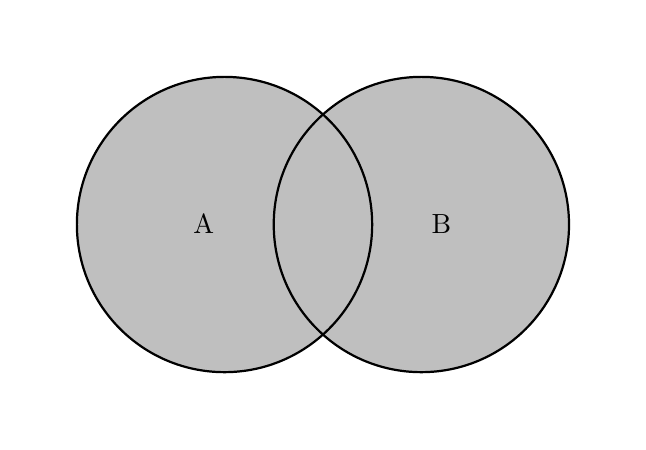
\begin{tikzpicture}[thick,scale=1.25]
\fill[white] (-2,-2) -- (4,-2) -- (4,2) -- (-2,2) -- cycle;
\fill[lightgray] (0,0) circle (1.5cm);
\fill[lightgray] (2,0) circle (1.5cm);
\draw (0,0) circle (1.5cm) node[left] {A};
\draw (2,0) circle (1.5cm) node[right] {B};
\end{tikzpicture}


\textbf{\large Intersection}

$P\cap Q$

All elements in both $P$ \textit{and} $Q$

\bigskip
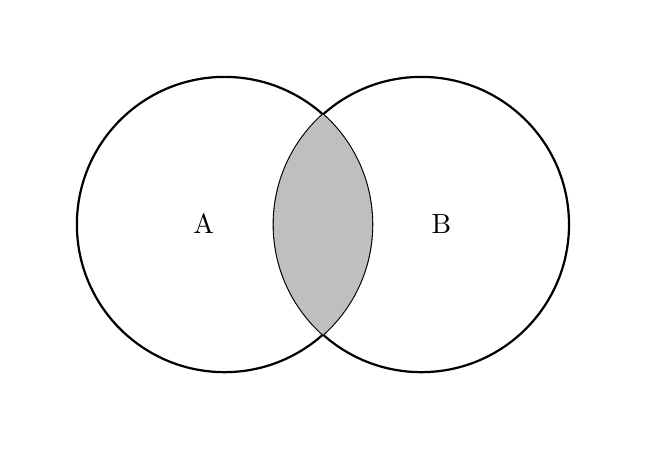
\begin{tikzpicture}[thick,scale=1.25]
\fill[white] (-2,-2) -- (4,-2) -- (4,2) -- (-2,2) -- cycle;
\draw (0,0) circle (1.5cm) node[left] {A};
\draw (2,0) circle (1.5cm) node[right] {B};
\clip (0,0) circle (1.5cm);
\fill[lightgray] (2,0) circle (1.5cm);
\end{tikzpicture}
\end{multicols}
\end{center}
\end{equationbox}

\bigskip
\begin{enumerate}[labelindent=*,style=multiline,leftmargin=*,label=\textbf{Example \arabic*:}]
\item Martha's has 15 cupcakes that are vanilla frosted and 10 cupcakes that are chocolate frosted. If two-thirds of Martha's cupcakes are both vanilla and chocolate frosted, how many cupcakes have vanilla frosting?
\vfill\item In the set of integers from 1 to 100 inclusively, how many numbers are divisible by 3 or 5 but not both?
\vfill\item Mr. Dropal has 16 students in his class. There are 10 male students. Half of all students are taking only Chinese and one-quarter are taking Chinese and French. If the class must take either French or Chinese, what proportion represents the maximum number of females taking only French?
\end{enumerate}

\vfill
\newpage
\begin{multicols*}{2}
\begin{outline}[enumerate]
\medium

\1 Mr. Carter has a garden of yellow, white, and red rose bushes. The proportion of red rose bushes to all other bushes is 0.4. When he buys an additional 4 red rose bushes, the proportion increases to 0.5. How many non-red rose bushes did Mr. Carter originally have?

\bigskip
\textbf{Equation/Strategy:} \hrulefill

\bigskip
\textbf{Solve:}

\vfill
\2 8
\2 12
\2 20
\2 24
\2 36

\midline

\1 The average (arithmetic mean) of a set of 5 positive integers is 10 and the median is 10. What is the largest possible value of the largest member of the set?

\bigskip
\textbf{Equation/Strategy:} \hrulefill

\bigskip
\textbf{Solve:}

\vfill
\2 10
\2 50
\2 22
\2 37
\2 40

\columnbreak
\advanced

\1 Helen has a box of 40 chocolates. The proportion cherry filled or coconut chocolates is 0.3, whereas the proportion of coconut or creme filled is 0.4. If the number of creme filled is twice the number of cherry filled and there is at least one cherry filled, what proportion of the box is coconut?

\bigskip
\textbf{Equation/Strategy:} \hrulefill

\bigskip
\textbf{Solve:}

\vfill
\2 0.075
\2 0.1
\2 0.15
\2 0.2
\2 0.25

\midline

\1 When a positive integer $n$ is divided by 4, the remainder is 3. When $n$ is divided by 5, the remainder is 1. How many values of $n$ are there from 1 to 40?

\bigskip
\textbf{Equation/Strategy:} \hrulefill

\bigskip
\textbf{Solve:}

\vfill
\2 0
\2 1
\2 2
\2 3
\2 4
\end{outline}
\end{multicols*}
	\section{Counting Techniques}

\bigskip
\textbf{General Equation:} 

\begin{tabularx}{\textwidth}{*2{@{}>{\centering\arraybackslash}X}}
\textbf{Permutations} & \textbf{Combinations}\\
\textit{Without Repetition} & \textit{Without Repetition}\\
$_nP_r=\frac{n!}{(n-r)!}$ & $_nC_r=\frac{n!}{r!(n-r)!}$\\[2em]
\textit{With Repetition} & \textit{With Repetition}\\
$n^r$ & $\frac{(n+r-1)!}{r!(n-1)!}$
\end{tabularx}

\vfill
\textbf{Example 1.} Mandy is throwing an ice cream party and has 3 flavors of ice cream and 4 different toppings. How many different combinations can her guests make?

\vfill
\textbf{Example 2.} Jerry is making a sundae with 3 scoops of ice cream. If he has 5 different flavors of ice cream, how many different combinations can Jerry make?

\vfill
\textbf{Example 3.} If a four-digit pin number contains the digits 0 to 9 where no digit can be repeated more than twice, how many different combinations for pin numbers are possible?

\vfill
\newpage
\begin{multicols*}{2}
\begin{outline}[enumerate]
\centerline{\large MEDIUM}

\1 If set A contains all even integers under twenty and set B contains all even prime numbers, then the set of common elements between set A and set B is

\bigskip
\textbf{Equation/Strategy:} \hrulefill

\bigskip
\textbf{Solve:}

\vfill
\2 \{\}
\2 \{0\}
\2 \{2\}
\2 \{0, 2\}
\2 All even numbers

\bigskip
\centerline{\rule{0.4\textwidth}{1pt}}

\bigskip
\1 If a four point star has 8 vertices, and an eight point star has 16 vertices, how many vertices does a 10 point star have?

\bigskip
\textbf{Equation/Strategy:} \hrulefill

\bigskip
\textbf{Solve:}

\vfill
\2 12
\2 16
\2 20
\2 24
\2 32

\columnbreak
\centerline{\large ADVANCED}

\1 A number of volleyballs compete in a tournament. If each team must play one another, and there are a total of 120 matches, how many teams competed?

\bigskip
\textbf{Equation/Strategy:} \hrulefill

\bigskip
\textbf{Solve:}

\vfill
\2 5 teams
\2 6 teams
\2 7 teams
\2 8 teams
\2 12 teams

\bigskip
\centerline{\rule{0.4\textwidth}{1pt}}

\bigskip
\1 An equilateral triangle is divided so that the midpoint of each line is the vertex of an inscribed triangle. If the process continues, how many triangles will there be after $n$ divisions?

\bigskip
\textbf{Equation/Strategy:} \hrulefill

\bigskip
\textbf{Solve:}

\vfill
\2 $2^n$
\2 $3^n$
\2 $4^n$
\2 $4n$
\2 $8n$
\end{outline}
\pagebreak
\end{multicols*}

\chapter{Algebra and Functions: Part I}


	\section[Algebraic Expressions]{Substitution and Simplifying Algebraic Expressions}

\textbf{General Equation}

\bigskip
\begin{equationbox}{Algebraic Properties}
\setlength{\columnseprule}{0pt}
For all real numbers $a,\ b$, and $c$,

\begin{center}
\begin{multicols}{2}
\textbf{Distributive Property}

$a(b+c)=ab+ac$

\columnbreak
\textbf{Transitive Property}

If $a=b$ and $b=c$, then $a=c$
\end{multicols}
\end{center}
\end{equationbox}

\bigskip
\begin{enumerate}[labelindent=*,style=multiline,leftmargin=*,label=\textbf{Example \arabic*:}]
\item If Sally has 6 boxes and each box has 12 books, how many books does Sally have?

\vfill\item Chase and Jill both collect stamps. If Jill has six less than twice the number of stamps than Chase does, how many stamps does Jill have if Chase has 24 stamps?

\vfill\item Townsville High School has 30 classrooms, each with 15 desks. If 80\% of desks are filled in 90\% of the classrooms and the other 10\% of the classrooms are 100\% full, how many students attend the school?
\end{enumerate}

\vfill
\newpage
\begin{multicols*}{2}
\begin{outline}[enumerate]
\medium

\1 Chris has a collection of 120 records which consists of jazz, blues, and classical records. If one-fourth of the records are jazz and one-third of the records are blues, how many of the records are classical?

\bigskip
\textbf{Equation/Strategy:} \hrulefill

\bigskip
\textbf{Solve:}

\vfill
\2 30
\2 40
\2 50
\2 60
\2 70

\midline

\1 The density, $d$, of an object is the ratio of its mass to its volume. If the volume of an object is halved and the mass is doubled, which expression represents the new density in terms of $d$?

\bigskip
\textbf{Equation/Strategy:} \hrulefill

\bigskip
\textbf{Solve:}

\vfill
\2 $1/4d$
\2 $1/2d$
\2 $d$
\2 $2d$
\2 $4d$

\columnbreak
\advanced

\1 Tommy is on the outer edge of a merry-go-round that moves at a constant speed. If $r$ is Tommy's distance from the center, and the merry-go-round makes $m$ full cycles during $n$ minutes, which expression represents Tommy's distance traveled in 1 hour?

\bigskip
\textbf{Equation/Strategy:} \hrulefill

\bigskip
\textbf{Solve:}

\vfill
\2 $\frac{mr\pi}{30n}$
\2 $\frac{mr^2\pi}{30n}$
\2 $\frac{120r\pi}{mn}$
\2 $\frac{120mr^2\pi}{n}$
\2 $\frac{120mr\pi}{n}$

\midline

\1 Bunny Slopes Co. is having a sale on winter wear of 20\% off. Tracy buys a pair of ski goggles and receives an additional 10\% off of the sale price. If the final cost of the goggles is \$90, how much did Tracy save?

\bigskip
\textbf{Equation/Strategy:}

\bigskip
\textbf{Solve:}

\vfill
\2 22
\2 25
\2 35
\2 38
\2 125
\end{outline}
\end{multicols*}
	\section[Linear Equations]{Solutions of Linear Equations and Inequalities}

\textbf{General Equation}

\bigskip
\begin{multicols}{2}
\setlength{\columnseprule}{0pt}
\begin{equationbox}{$\boldsymbol{y-}$intercept}
The \textit{\bfseries $\boldsymbol{y-}$intercept} of a line is the point where the graph of the line intersects the $y-$axis. Its coordinate is given by the point $(0, b)$ where $b$ is determined by the equation of the line $y=mx+b$.

\phantom{}
\end{equationbox}

\begin{equationbox}{$\boldsymbol{x-}$intercept}
The \textit{\bfseries $\boldsymbol{x-}$intercept} of a line is the point where the graph of the line intersects the $x-$axis. Its coordinate is given by the point $\left(-\frac{m}{b},0\right)$ where $m$ and $b$ are determined by the equation of the line $y=mx+b$.
\end{equationbox}
\end{multicols}

\bigskip
\begin{enumerate}[labelindent=*,style=multiline,leftmargin=*,label=\textbf{Example \arabic*:}]
\item If the cost of a cab has a base fare of \$2.50 and \$0.40 per mile, how much does a 10 mile ride cost?

\vfill\item The cost of tablet devices has dropped an average of 3\% of the original price every quarter of a year. After how long will the cost of a tablet be less than half of the original cost?

\vfill\item The population of Summerville increases at a constant annual rate. The population was recorded in January 2008 as 362,000 and again in July 2010 as 384,000. What is the annual rate of growth of the population?
\end{enumerate}

\vfill
\newpage
\begin{multicols*}{2}
\begin{outline}[enumerate]
\medium

\1 The speed of a minute hand moves at a constant speed of $1/60$ rpm (revolutions per minute). If the current time is 4:00 pm and the minute hand has made 1.75 revolutions, what time was it first recorded at?

\bigskip
\textbf{Equation/Strategy:} \hrulefill

\bigskip
\textbf{Solve:}

\vfill
\2 2:15 pm
\2 2:25 pm
\2 2:45 pm
\2 3:15 pm
\2 3:25 pm

\midline

\1 Both Terri and Sam are shorter than Sissy, and Sissy and Hector is shorter than Roy. Which of the following must be true?

\begin{enumerate}[label=\Roman*.]
\item Terri is shorter than Sam
\item Sissy is shorter than Hector
\item Sam is shorter than Roy
\end{enumerate}

\bigskip
\textbf{Equation/Strategy:} \hrulefill

\bigskip
\textbf{Solve:}

\vfill
\2 I only
\2 II only
\2 III only
\2 I and II
\2 II and III

\columnbreak
\advanced

\1 A chemical reaction results in the release the constant release of 70 joules of energy over a 14 minute period. If the total initial amount of energy in the system was 370 joules, how long will it take for the system to release all of its energy?

\bigskip
\textbf{Equation/Strategy:} \hrulefill

\bigskip
\textbf{Solve:}

\vfill
\2 1 hour 10 minutes
\2 1 hour 14 minutes
\2 1 hour 17 minutes
\2 1 hour 24 minutes
\2 5 hours 17 minutes

\vfill\vfill\phantom{}
\newpage
\1 The number of students at Mainsville School with cellphones increases at a constant rate of $n$ students per year. If the number of students with cellphones in January 2010 is 200 and the population of the student body is $p$, which expression represents the proportion of students with cellphones after $m$ months?

\bigskip
\textbf{Equation/Strategy:} \hrulefill

\textbf{Solve:}

\vfill
\2 $\frac{mn}{p+200}$
\2 $\frac{mn}{p-200}$
\2 $\frac{mn+200}{p}$
\2 $\frac{mn+2400}{p}$
\2 $\frac{mn+2400}{12p}$
\vfill\vfill\phantom{}
\end{outline}
\end{multicols*}
	\include{04.3_AlgebraFunctionsI}
	\section[System of Equations]{Systems of Equations and Inequalities}

\bigskip
\textbf{General Equation:} 

\bigskip
\begin{tabularx}{\textwidth}{*2{@{}>{\centering\arraybackslash}X}}
Parallel Lines & Perpendicular Lines\\
$m_1 = m_2$ & $m_1 \cdot m_2 = -1$
\end{tabularx}

\vfill
\begin{enumerate}[labelindent=*,style=multiline,leftmargin=*,label=\textbf{Example \arabic*:}]
\item Plane A and plane B are flying parallel to one another. If after 20 minutes, plane A has risen an altitude of 2000 m, how much has the altitude of plane B has risen in 30 minutes?

\vfill\item When Johnny has $x$ nickels and $y$ dimes, his total is \$3. When he has $y$ nickels and $x$ dimes, his total increases by \$0.75. How many nickel and dimes did Johnny start off with?

\vfill\item Two cars starting at the same intersection begin traveling perpendicular to one another. If the first car travels north west at a $25^\circ$ angle of the point of intersection, what is the direction of the second car?
\end{enumerate}

\vfill
\newpage
\begin{multicols*}{2}
\begin{outline}[enumerate]
\medium

\1 A coffee costs \$2.5 and a muffin costs \$3. If Tasha has \$11 and makes a purchase, what is the least amount of change she can receive?

\bigskip
\textbf{Equation/Strategy:} \hrulefill

\bigskip
\textbf{Solve:}

\vfill
\2 \$0.00
\2 \$0.50
\2 \$1.00
\2 \$1.50
\2 \$2.00

\midline

\1 Stacy and Ann enter a relay race that consists of 3 events, each worth 10 points. If Stacey earned 8 points and 9 points in the first two events, what is the least number of points she will need to earn in the third event to win if Ann received received a 23 points total?

\bigskip
\textbf{Equation/Strategy:} \hrulefill

\bigskip
\textbf{Solve:}

\vfill
\2 6
\2 7
\2 10
\2 23
\2 24

\columnbreak
\advanced

\1 Two planes leave from parallel terminals. If plane A travels northwest at 400 mph, and plane B travels northwest 600 mph 4 hours later, by what time will the second plane have equal distance traveled as the first plane?

\bigskip
\textbf{Equation/Strategy:} \hrulefill

\bigskip
\textbf{Solve:}

\vfill
\2 2
\2 8
\2 4
\2 12
\2 48

\midline

\1 A coyote is chasing roadrunner in a parallel path. If the roadrunner and coyote are running at a constant rate of 30 mph and the roadrunner has a 20 mile gain on the coyote, how much faster will the coyote need to run if he is going to catch up to the roadrunner in 2 hours?

\bigskip
\textbf{Equation/Strategy:} \hrulefill

\bigskip
\textbf{Solve:}

\vfill
\2 10 mph
\2 20 mph
\2 25 mph
\2 30 mph
\2 40 mph
\end{outline}
\end{multicols*}
	\section{Equations of Lines}

\bigskip
\textbf{General Equation:}

\begin{center}
Slope-Intercept Form of a Line

$y=mx+b$
\end{center}

\vfill
\textbf{Example 1.} Sunshine taxi charges a base fare of \$2.60 and \$0.40 for every quarter mile. If Elle's ride is 5 miles, how much is her ride?

\vfill
\textbf{Example 2.} A parking lot charges \$10 for the first 4 hours and \$2 up to every additional hour. If George leaves his car for 8 and a half hours, how much is he charged?

\vfill
\textbf{Example 3.} Moe's dad will give him \$1 for every $x$ points over 50 on his math test, where $x$ is a whole number of points. Moe received 86 points on his math test and earned \$12. How many points does Moe need to earn \$1?

\vfill
\newpage
\begin{multicols*}{2}
\begin{outline}[enumerate]
\centerline{\large MEDIUM}

\1 Travis is a car salesman and earns \$10 an hour plus a flat commission fee for each car he sells. If Travis works 30 hours and has earned \$1,000 in a week, how much does Travis earn in commission per car if he sells 4 cars?

\bigskip
\textbf{Equation/Strategy:} \hrulefill

\bigskip
\textbf{Solve:}

\vfill
\2 80
\2 160
\2 320
\2 360
\2 640

\bigskip
\centerline{\rule{0.4\textwidth}{1pt}}

\bigskip
\1 Cherry is setting up a can drive at her school. For every 50 cans after 100 she collects, the donation center will give her one ticket to an amusement park. If Cherry wants a total of 10 tickets, what is the least number of cans she will need to collect?

\bigskip
\textbf{Equation/Strategy:} \hrulefill

\bigskip
\textbf{Solve:}

\vfill
\2 500
\2 600
\2 1050
\2 1500
\2 5100

\columnbreak
\centerline{\large ADVANCED}

\1 The value of a car depreciates every year at a constant rate of $p$\% of the total value. If the initial value of the car is $d$ dollars, what is the current value of the car after $m$ months?

\bigskip
\textbf{Equation/Strategy:} \hrulefill

\bigskip
\textbf{Solve:}

\vfill
\2 $d-pm$
\2 $d-\frac{pm}{12}$
\2 $d-\frac{pm}{100}$
\2 $d-\frac{pm}{1200}$
\2 $d\left(1-\frac{pm}{1200}\right)$

\bigskip
\centerline{\rule{0.4\textwidth}{1pt}}
\1 The value of an interior angle of a regular $n$-gon increases as a linear function of $n$. If an interior angle of a 4-gon is $90^\circ$ and a 6-gon is $120^\circ$, what is the sum of all interior angles of an $n$-gon whose interior angles are each $144^\circ$?

\bigskip
\textbf{Equation/Strategy:} \hrulefill

\bigskip
\textbf{Solve:}

\vfill
\2 10
\2 12
\2 144
\2 576
\2 1440
\end{outline}
\end{multicols*}

\chapter{Algebra and Functions: Part II}
	\section{Absolute Value}

\bigskip
\textbf{General Equation}

\bigskip
\begin{equationbox}{Properties of Absolute Values}
\setlength{\columnseprule}{0pt}

For any value $a$ and $b$,

\begin{center}
\begin{multicols}{2}
$|a-b|=|b-a|$

$|a\cdot b|=|a|\cdot|b|$
\end{multicols}
\end{center}
\end{equationbox}

\vfill
\begin{enumerate}[labelindent=*,style=multiline,leftmargin=*,label=\textbf{Example \arabic*:}]
\item Dallas walks to her friends house 6 blocks north of her house. She then walks 3 blocks south to visit Francis. What is the total distance traveled by Dallas?

\vfill\item A train travels east $x$ miles, then travels west $y$ miles. What expression gives the net distance traveled by the train?

\vfill\item A ball is thrown upward from the ground and travels a distance of $n$ meters, then bounces to a height half of the previous. If the ball bounces 5 times, what is the total distance traveled by the ball in terms of $n$?
\end{enumerate}

\vfill
\newpage
\begin{multicols*}{2}
\begin{outline}[enumerate]
\medium

\1 A toy train travels on a circular path with a diameter of 10 feet. If Ellen runs the train forward 2.5 revolutions, then in reverse for 1.5 revolutions, what is the total distance traveled by the train?

\bigskip
\textbf{Equation/Strategy:} \hrulefill

\bigskip
\textbf{Solve:}

\vfill
\2 $5\pi$ meters
\2 $10\pi$ meters
\2 $40\pi$ meters
\2 $20\pi$ meters
\2 $100\pi$ meters

\midline

\1 If two objects are falling at the same speed, $s$ meters per second, what is the total distance over $t$ seconds traveled by both objects if the distance between them is $d$ units?

\bigskip
\textbf{Equation/Strategy:} \hrulefill

\bigskip
\textbf{Solve:}

\vfill
\2 $|st|$
\2 $|st-d|$
\2 $|2sd|$
\2 $|2st|$
\2 $|2st-d|$

\columnbreak
\advanced

\1 Lucky and Sunshine are two horses that are running in opposite directions of each other. If Lucky's velocity is $p$ mph and is twice the velocity of Sunshine, what is the distance between the horses after $t$ minutes?

\bigskip
\textbf{Equation/Strategy:} \hrulefill

\bigskip
\textbf{Solve:}

\vfill
\2 $\left|\frac{pt}{60}\right|+\left|\frac{pt}{120}\right|$
\2 $\left|\frac{pt}{60}+\frac{pt}{120}\right|$
\2 $\left|\frac{pt}{30}\right|+\left|\frac{pt}{60}\right|$
\2 $\left|\frac{pt}{30}+\frac{pt}{60}\right|$
\2 $\left|\frac{pt}{30}\right|+\left|\frac{pt}{120}\right|$

\midline

\1 A ping pong ball travels a constant velocity of $h$ inches per $s$ seconds with every successive hit. What is the ping pong speed if it travels $g$ feet in $m$ minutes?


\bigskip
\textbf{Equation/Strategy:} \hrulefill

\bigskip
\textbf{Solve:}


\begin{enumerate}[label=(\Alph*)]
\setlength{\columnseprule}{0pt}
\begin{multicols}{2}
\item $\left|\frac{5gh}{ms}\right|$
\item $\left|\frac{gh}{5ms}\right|$
\vfill

\item $\left|\frac{5hm}{gs}\right|$
\item $\left|\frac{hm}{5gs}\right|$
\item $\left|\frac{gs}{5hm}\right|$
\end{multicols}
\end{enumerate}
\end{outline}

\end{multicols*}
	\include{05.2_AlgebraFunctionsII}
	\section{Quadratic Equations}

\bigskip
\textbf{General Equation:} If $f(x)$ is a quadratic functions with roots $r$ and $s$, then the coordinate of the vertex (maximum or minimum) is

\[\left(\frac{s-r}{2},\ f\left(\frac{s-r}{2}\right)\right)\]

\vfill
\begin{enumerate}[labelindent=*,style=multiline,leftmargin=*,label=\textbf{Example \arabic*:}]
\item Reese jumps, starting from the ground, and reaches a maximum height of 6 feet at 3 seconds. How long does the trip take from when she first jumped until she returned back to the ground?

\vfill\item A cannonball is fired from ground-level and hits the ground after $t$ seconds. If the maximum height is $h$ ft, write the coordinate that expresses the maximum of the cannonball's trajectory.

\vfill\item The sum of two integers $x$ and $y$ is $m$ and the product of the two integers is $n$. What is $n$ in terms of $x$?
\end{enumerate}

\vfill
\newpage
\begin{multicols*}{2}
\begin{outline}[enumerate]
\medium

\1 Stacey is making a rectangular garden for her rose bushes. If the perimeter needs to be 100 cm, what is the maximum area she can enclose?

\bigskip
\textbf{Equation/Strategy:} \hrulefill

\bigskip
\textbf{Solve:}

\vfill
\2 25 cm$^2$
\2 50 cm$^2$
\2 100 cm$^2$
\2 500 cm$^2$
\2 625 cm$^2$

\midline

\1 For two integers $p$ and $q$, the sum of their squares is equal to the square of their sum. What is the value of $pq$?

\bigskip
\textbf{Equation/Strategy:} \hrulefill

\bigskip
\textbf{Solve:}

\vfill
\2 0
\2 1
\2 2
\2 3
\2 4

\columnbreak
\advanced

\1 A sector of a circle is inscribed in a square. If the radius of the circle is equal to the side length of the square, $s$, what is the area of the inscribed sector in terms of $s$?

\bigskip
\textbf{Equation/Strategy:} \hrulefill

\bigskip
\textbf{Solve:}

\vfill
\2 $\pi s^2/4$
\2 $\pi s^2/2$
\2 $s^2/4$
\2 $s^2/2-\pi$
\2 $s^2-\pi/4$

\midline

\1 Andres has 1.2 kilometers of fencing he wishes to use to create two adjacent pens for his sheep and his goats. If he uses the fencing for the perimeter and a divider in the middle of the entire pen, what is the length, in meters of the shortest side? (1 kilometer = 1000 meters)

\bigskip
\textbf{Equation/Strategy:} \hrulefill

\bigskip
\textbf{Solve:}

\vfill
\2 150 m
\2 300 m
\2 400 m
\2 600 m
\2 750 m
\end{outline}
\end{multicols*}
	\section[Rational \& Radical]{Rational and Radical Equations}

\bigskip
\textbf{General Equation:}

\bigskip
If $\frac{a}{b}=\frac{c}{d}$, then

\bigskip
\begin{itemize}[label=$\bullet$]
\item $ad=bc$

\bigskip
\item $\frac{a}{c}=\frac{b}{d}$
\end{itemize}

\vfill
\begin{enumerate}[labelindent=*,style=multiline,leftmargin=*,label=\textbf{Example \arabic*:}]
\item If the sequence $x$, \shortline, $y$ has a common ratio between each term, what is the value of the missing term?

\vfill\item A three digit number is evenly divided by a two digit number such that the quotient is a perfect square. What is the smallest such three digit number and two digit number pair?

\vfill\item For an integer $n$, the square root and cube root are both integers. If the square root and cube root of $n$ are distinct, what is the smallest sum of both roots of such a number?
\end{enumerate}

\vfill
\newpage
\begin{multicols*}{2}
\begin{outline}[enumerate]
\medium

\1 The probability of choosing a red marble is 1 out of $p$ marbles and the probability of choosing a green marble is 1 out of $q$ marbles. Which expression represents the probability of choosing a red or a green marble?

\bigskip
\textbf{Equation/Strategy:} \hrulefill

\bigskip
\textbf{Solve:}

\vfill
\2 $(p+q)/pq$
\2 $1/pq$
\2 $2/pq$
\2 $p+q$
\2 $(1-p)(1-q)$

\midline

\1 Benjamin is missing cards in his deck of cards. If in his deck of 50 cards there are $x$ kings and $y$ queens. What are the odds of choosing a queen and a king?

\bigskip
\textbf{Equation/Strategy:} \hrulefill

\bigskip
\textbf{Solve:}

\vfill
\2 $xy/50$
\2 $(x+y)/50$
\2 $2500/xy$
\2 $(x+y)/2500$
\2 $xy/2500$

\columnbreak
\advanced

\1 The ratio of the sides of a rectangle is $a:b$. If one is added to both sides, the new ratio of sides is $b:a$. Which of the following must be true?

\begin{enumerate}[label=\Roman*.]
\item The rectangle is a square
\item The area is $a^2$
\item The side length is 1
\end{enumerate}

\bigskip
\textbf{Equation/Strategy:} \hrulefill

\bigskip
\textbf{Solve:}

\vfill
\2 I is true
\2 II is true
\2 III is true
\2 I and II are true
\2 I, II, and III are true

\midline

\1 A square is inscribed in a circle. If the radius of the circle double, by what factor does the side length of the square grow?

\bigskip
\textbf{Equation/Strategy:} \hrulefill

\bigskip
\textbf{Solve:}

\vfill
\2 2
\2 $\sqrt2$
\2 4
\2 $2\sqrt2$
\2 $4\sqrt2$
\end{outline}
\end{multicols*}
	\section[Algebraic Functions]{Concepts of Algebraic Functions}

\bigskip
\textbf{General Equation}

\bigskip
\begin{equationbox}{Coordinates}
\textbf{Definition:} If $f(a)=b$, then $(a,b)$ is a coordinate of the graph of $f$.
\end{equationbox}

\bigskip
\begin{enumerate}[labelindent=*,style=multiline,leftmargin=*,label=\textbf{Example \arabic*:}]
\item If Timmy sells less lemonade in week $x$ than in week $y$ and Timmy's sales has increased every week, what relationship describes $y$ to $x$?

\vfill\item Luckystar is a horse that races in the Belmont racetrack. If Luckystar runs at $x$ mph at time $p$ and again at time $q$, what is his increase in average speed over the interval from $p$ to $q$?

\vfill\item If Arnold has $3\times3, 4\times4$, and $5\times5$ cubes, what is the least number of cubes Arnold will need to make a building that is 27 units high?

\vfill\item Lindsey and Ricky have separate college tuition funds created on a Monday. Lindsey's account starts at an initial amount of \$0.50 and the total doubles every day, whereas Ricky's college tuition starts at \$1 initially and the total doubles every day. On what day will Lindsey begin having greater amounts in her account than Ricky will have in his account?
\end{enumerate}

\vfill
\newpage
\begin{multicols*}{2}
\begin{outline}[enumerate]
\medium

\1 If the amount of bacteria in a colony doubles every hour, which of the following cannot be a relative factor of the population of bacteria?

\bigskip
\textbf{Equation/Strategy:} \hrulefill

\bigskip
\textbf{Solve:}

\vfill
\2 1/2
\2 0
\2 1
\2 2
\2 8

\midline

\1 $f$ has the property that $f(\square)=\clubsuit$ and $f(\clubsuit)=\square$ for all $\clubsuit$ and $\square$. Which of the following represents the equation for $f$ in terms of $x$?

\bigskip
\textbf{Equation/Strategy:} \hrulefill

\bigskip
\textbf{Solve:}

\vfill
\2 $f(x)=x$
\2 $f(x)=x^2$
\2 $f(x)=0$
\2 $f(x)=1$
\2 $f(x)=\sqrt{x}$

\columnbreak
\advanced

\1 The odds of choosing a prime number out of $x$ terms is $m$ and the odds of choosing and even number out of the same $x$ terms is $n$. What are the odds of choosing an even prime out of $x^2$ terms?

\bigskip
\textbf{Equation/Strategy:} \hrulefill

\bigskip
\textbf{Solve:}

\vfill
\2 $1/mn$
\2 $1/x$
\2 $1/x^2$
\2 $1/(m+n)$
\2 Cannot be determined

\midline

\1 If Kat is on a swing that starts at a height of $h$ off the ground and reaches the ground after $t/3$ seconds, at what position will she be at $15t$ relative to her beginning position?

\bigskip
\textbf{Equation/Strategy:} \hrulefill

\bigskip
\textbf{Solve:}

\vfill
\2 $h$
\2 $-h$
\2 0
\2 $2h$
\2 $-2h$
\end{outline}
\end{multicols*}
	\section{Newly Defined Symbols}
\bigskip
\textbf{General Equation} 

\bigskip
\begin{equationbox}{Function}
\textbf{Definition:} $y=f(x)$ indicates that the value of $y$ is a function of it's input $x$. For each value of $x$ there is one and only one value of $y$.
\end{equationbox}

\bigskip
\begin{enumerate}[labelindent=*,style=multiline,leftmargin=*,label=\textbf{Example \arabic*:}]
\item If $f\otimes g$ is defined as $f\cdot g-(f+g)$, what is the value of $g$ in terms of $f$ so that $f\otimes g=0$?

\vfill\item If $f\%g$ is defined as the remainder of $f$ when divided by $g$, what is $(x-4x+4)\%(x-2)$?

\vfill\item $S$ is a set with elements $s_1, s_2,\ldots s_n$. Let $S\bullet S$ be defined as $s_1\cdot s_1+s_2\cdot s_2+\ldots s_n\cdot s_n$. If $S\bullet S=0$ what must be true of the elements of $S$? Justify your answer.
\end{enumerate}

\vfill
\newpage
\begin{multicols*}{2}
\begin{outline}[enumerate]
\medium

\1 The function $f(n)=n\cdot f(n-1)$ for all $n>1$ where $f(1)=1$. What is the value of $f(5)$?

\bigskip
\textbf{Equation/Strategy:} \hrulefill

\bigskip
\textbf{Solve:}

\vfill
\2 1
\2 5
\2 40
\2 50
\2 120

\midline

\1 Let $(a,b)$ be equal to the value of the greatest common factor between $a$ and $b$. What is the value of $(x^2-2x+1, x^2+3x-4)$?

\bigskip
\textbf{Equation/Strategy:} \hrulefill

\bigskip
\textbf{Solve:}

\vfill
\2 0
\2 1
\2 x
\2 x-1
\2 x+1

\columnbreak
\advanced

\1 $\lfloor x\rfloor$ is defined as the greatest integer less than or equal to $x$ whereas $\lceil x\rceil$ is defined as the least integer greater than or equal to $x$. If $x$ is not an integer, what is the value of $\lfloor\lceil x\rceil\rfloor$?

\bigskip
\textbf{Equation/Strategy:} \hrulefill

\bigskip
\textbf{Solve:}

\vfill
\2 1
\2 0
\2 $x$
\2 $x^2$
\2 Cannot be determined

\midline

\1 The ternary operation $\clubsuit@\diamondsuit@\spadesuit$ is defined as $\clubsuit=\diamondsuit$ when $\clubsuit\geq0$, and $\clubsuit=\spadesuit$ when $\clubsuit<0$. What is the simplified value of $\heartsuit^2@-\left|\heartsuit^2\right|@\sqrt{(-\heartsuit^2)^2}$?

\bigskip
\textbf{Equation/Strategy:} \hrulefill

\bigskip
\textbf{Solve:}

\vfill
\2 $-a^2$
\2 $a^2$
\2 $\left|-a^2\right|$
\2 $\sqrt{a^4}$
\2 $\sqrt{-a^4}$
\end{outline}
\end{multicols*}

\chapter{Geometry and Measurement: Part I}
	\section[Polygons]{Area and Perimeter of a Polygon}
\textbf{General Equation:}

\begin{center}
\begin{multicols}{2}
\setlength{\columnseprule}{0pt}
Area

The measure of the surface of a two-dimensional shape

Perimeter

The measure of the distance around a two-dimensional shape
\end{multicols}
\end{center}

\vfill\textbf{Example 1:} The lengths of an $n$-sided figure are each doubled. If the perimeter of the original $n$-sided figure was $P$, what is the value of the new perimeter?

\vfill\textbf{Example 2:} A circle inscribed in a box has a radius equal to half of the diameter of the box. What area of the circle is not in the square if the radius is 1?

\vfill\textbf{Example 3:} A pizza box has a perimeter that is 1.5 times the circumference of the pizza. If the pizza has a diameter of 16 inches, what is the difference between the perimeter of the box and the circumference of the pizza?

\vfill
\newpage
\begin{multicols*}{2}
\begin{outline}[enumerate]
\centerline{\large MEDIUM}

\1 A square is inscribed in a circle. If the area of the square is 9 sq. in., what is the difference between the circumference of the circle and the perimeter of the square?

\bigskip
\textbf{Equation/Strategy:} \hrulefill

\bigskip
\textbf{Solve:}

\vfill
\2 $3\sqrt{2}\pi-12$
\2 $12-3\sqrt{2}\pi$
\2 $6\sqrt{2}\pi-12$
\2 $12-6\sqrt{2}\pi$
\2 $3$

\bigskip
\centerline{\rule{0.4\textwidth}{1pt}}

\bigskip
\1 A right triangle has an area of $b$ sq. units. If a rectangle has a height equivalent to the height of the right triangle, and a base equivalent to twice the base of the right triangle, what is the area of the rectangle in terms of $a$?

\bigskip
\textbf{Equation/Strategy:} \hrulefill

\bigskip
\textbf{Solve:}

\vfill
\2 $a$
\2 $2a$
\2 $4a$
\2 $a^2$
\2 $2a^2$

\columnbreak
\centerline{\large ADVANCED}

\1 A rectangle whose width is twice its height is inscribed in a semicircle whose radius is equal to width of the rectangle. If $h$ is the height of the rectangle, which expression represents the area of the semicircle not in the area of the rectangle?

\bigskip
\textbf{Equation/Strategy:} \hrulefill

\bigskip
\textbf{Solve:}

\vfill
\2 $2w^2(\pi-1)$
\2 $2w^2(9w^2\pi-1)$
\2 $2w^2(2\pi-1)$
\2 $2w^2(2\pi-1)$
\2 $w^2(\pi-2)$

\centerline{\rule{0.4\textwidth}{1pt}}

\1 Triangle $A$ is inscribed in equilateral triangle $B$ so that the vertices of $A$ are the midpoints of the sides of $B$. If the area of $B$ is 12 sq. units, what is the area of the $B$ with $A$ removed?

\bigskip
\textbf{Equation/Strategy:}

\bigskip
\textbf{Solve:}

\vfill
\2 6 sq. units
\2 7 sq. units
\2 8 sq. units
\2 9 sq. units
\2 12 sq. units
\end{outline}
\end{multicols*}
	\include{06.2_GeometryMeasurementI}
	\section[Volumes]{Volume of a Box, Cube, and Cylinder}

\textbf{General Equation}

\bigskip
\begin{equationbox}{Volume Equations}
\setlength{\columnseprule}{0pt}

\begin{center}
\begin{multicols}{3}
\textbf{Volume of a Box}

$V=l\times w\times h$

\textbf{Volume of a Cube}

$V=s^3$

\textbf{Volume of a Cylinder}

$V=\pi r^2h$
\end{multicols}
\end{center}
\end{equationbox}

\bigskip
\begin{enumerate}[labelindent=*,style=multiline,leftmargin=*,label=\textbf{Example \arabic*:}]
\item Kallie is filling her bookshelf with books that are $8\times5\times2$ in\textsuperscript{3}. If Kallie has 16 such books, how much volume do the books occupy?

\vfill\item A large cube is made by stacking smaller $4\times4$ cubes. What is the total volume of the large cube?

\vfill\item Pete stacks pizza pies on each other in a freezer for later heating. The pizzas are 2 inches thick and have a diameter of 16 inches. What volume do 10 pizzas occupy?
\end{enumerate}

\vfill
\newpage
\begin{multicols*}{2}
\begin{outline}[enumerate]
\medium

\1 A rectangular box has a volume of 36 in\textsuperscript{3} If cubes of side length 2 are placed into the rectangular box, what is the least amount of volume of the box not filled by the cubes?

\bigskip
\textbf{Equation/Strategy:} \hrulefill

\bigskip
\textbf{Solve:}

\vfill
\2 0 in\textsuperscript{3}
\2 2 in\textsuperscript{3}
\2 4 in\textsuperscript{3}
\2 6 in\textsuperscript{3}
\2 8 in\textsuperscript{3}

\midline

\1 A cylinder is placed in a rectangular box so that the diameter of the cylinder is the width and height of the rectangle. What is the ratio of volume of the cylinder to the volume of the box?

\bigskip
\textbf{Equation/Strategy:} \hrulefill

\bigskip
\textbf{Solve:}

\vfill
\2 $4-\pi$
\2 $\frac{4}{\pi}$
\2 $\frac{\pi}{4}$
\2 $\frac{8}{\pi}$
\2 $\frac{\pi}{8}$

\columnbreak
\advanced

\1 A cube of volume $V$ of integer side length $s$ is split into 6 smaller rectangular boxes of equal volume. What is the value of $V$ if it is the smallest such cube?

\bigskip
\textbf{Equation/Strategy:} \hrulefill

\bigskip
\textbf{Solve:}

\vfill
\2 6
\2 36
\2 64
\2 125
\2 216

\midline

\1 Cubic blocks are stored in a cylindrical container so that the diagonal length of the cube is the diameter length of the cylinder. If the height of the cylinder is 5 times the radius, what is the most number of cubes that fit into the cylinder?

\bigskip
\textbf{Equation/Strategy:}

\bigskip
\textbf{Solve:}

\vfill
\2 1
\2 2
\2 3
\2 4
\2 5
\end{outline}
\end{multicols*}
	\section[Special Triangles]{Pythagorean Theorem and Special Properties of Isosceles, Equilateral, and Right Triangles}

\textbf{General Equation:}

\begin{center}
The Pythagorean Theorem

$a^2+b^2=c^2$
\end{center}

\vfill
\begin{enumerate}[labelindent=*,style=multiline,leftmargin=*,label=\textbf{Example \arabic*:}]
\item The perimeter of an equilateral triangle is 16 cm. What is the triangle's area?

\vfill\item Gretchen and Samuel leave school. Gretchen walks $45^\circ$ due south west and Samuel walks $45^\circ$ due south east. If they each live a quarter mile away from school, what is the distance between their houses?

\vfill\item A 13 ft ladder is propped up against a wall. If the base of the ladder to the base of the wall is equidistant of the top of the ladder to the base of the wall, what is the difference between the length of the ladder and the base of the ladder to the base of the wall?
\end{enumerate}

\vfill
\newpage
\begin{multicols*}{2}
\begin{outline}[enumerate]
\medium

\1 The area of an equilateral triangle is 16 cm\textsuperscript{2}. What is the triangle's perimeter to the nearest hundredth?

\bigskip
\textbf{Equation/Strategy:} \hrulefill

\bigskip
\textbf{Solve:} 

\vfill
\2 3.04
\2 6.07
\2 6.08
\2 18.23
\2 18.24

\midline

\1 The ratio of the sides of a right triangle are in a proportion of $2:3:x$ where $x$ is the proportion of the longest side. If the hypotenuse is 27 units long, what the area of the triangle to the nearest hundredth?

\bigskip
\textbf{Equation/Strategy:} \hrulefill

\bigskip
\textbf{Solve:}

\vfill
\2 168.23
\2 168.20
\2 243
\2 292.04
\2 292.05

\columnbreak
\advanced

\1 The hypotenuse of a right triangle is twice as long as the shortest side. If the length of the longer leg is 10 cm, what is the perimeter of the triangle?

\bigskip
\textbf{Equation/Strategy:} \hrulefill

\bigskip
\textbf{Solve:}

\vfill
\2 $10+10\sqrt{3}$
\2 $20+\sqrt{3}$
\2 $20+10\sqrt{3}$
\2 $30+10\sqrt{3}$
\2 30

\midline

\1 The side lengths of a rectangle are in a proportion of $a:a+4$. If the perimeter is 76 sq. units, what is the length of the hypotenuse?

\bigskip
\textbf{Equation/Strategy:}

\bigskip
\textbf{Solve:}

\vfill
\2 12 units
\2 16 units
\2 24 units
\2 20 units
\2 40 units
\end{outline}
\end{multicols*}

\chapter{Geometry and Measurement: Part II}
	\section[Linear Relationships]{Properties of Parallel and Perpendicular lines}

\textbf{General Equation}

\bigskip
\begin{equationbox}{Parallel and Perpendicular Lines}
\setlength{\columnseprule}{0pt}
For lines $L_1$ and $L_2$ with slopes $m_1$ and $m_2$ respectively

\begin{center}
\begin{multicols}{2}
\textbf{Parallel Lines}

$m_1=m_2$

\columnbreak
\textbf{Perpendicular Lines}

$m_1\cdot m_2=-1$
\end{multicols}
\end{center}
\end{equationbox}

\bigskip
\begin{enumerate}[labelindent=*,style=multiline,leftmargin=*,label=\textbf{Example \arabic*:}]
\item Two planes are traveling parallel to one another. If the first plane travels in a direction 30 miles north and 40 miles east of where it began, and the second plane travels 60 miles north of where it began, how far east must it travel in order to remain parallel to the first plane?

\vfill\item Two cars starting at the same location are traveling perpendicular to one another. What is the distance between the two cars if the first car has traveled 30 miles in one hour and the second car has traveled 40 miles in one hour?

\vfill\item A frog's tongue shoots straight up into the air to catch a fly that is flying horizontally. If the distance from the fly's speed is 6 meters per second and the speed between the frog and the fly is 20 meters per 2 seconds, how fast must the frog's tongue move in order to catch the fly?
\end{enumerate}

\vfill
\newpage
\begin{multicols*}{2}
\begin{outline}[enumerate]
\medium

\1 Roads A and B are parallel roads. If Road C runs perpendicular to road A, which of the following must be true?

\begin{enumerate}[label=\Roman*.]
\item Road C is perpendicular to Road B
\item Road A and C form a $90^\circ$ angle
\item The distance between Road A and Road B is uniform
\end{enumerate}

\bigskip
\textbf{Equation/Strategy:} \hrulefill

\bigskip
\textbf{Solve:}

\vfill
\2 I only
\2 II only
\2 III only
\2 I and II are true
\2 I, II, and III are true

\midline

\1 Two dogs are running perpendicular paths, starting at the same location. If the first dog runs $m$ meters in 5 minutes, and the second dog runs $m$ meters in 10 minutes, which of the following represents the distance between the dogs after 10 minutes?

\bigskip
\textbf{Equation/Strategy:} \hrulefill

\bigskip
\textbf{Solve:}

\vfill
\2 $m\sqrt{2}$
\2 $m\sqrt{3}$
\2 $\sqrt{2m^2+m^2}$
\2 $\sqrt{\frac{m}{2}^2+m^2}$
\2 $\sqrt{4m^2+m^2}$

\columnbreak
\advanced

\1 A set of parallel roads runs perpendicular to a second set of parallel roads. If the distance between each intersection along the road is at most $m$ km, which of the following cannot be the distance between diagonal intersections?

\bigskip
\textbf{Equation/Strategy:} \hrulefill

\bigskip
\textbf{Solve:}

\vfill
\2 $m$
\2 $2m$
\2 $\frac{m}{2}$
\2 $\frac{m\sqrt{2}}{2}$
\2 $m\sqrt{2}$

\midline

\1 A pair of parallel chords are inscribed in a circle, equidistant from the center. If the distance between the chords is equal to the radius, $r$, what is the length each chord in terms of $r$?

\bigskip
\textbf{Equation/Strategy:}

\bigskip
\textbf{Solve:}

\vfill
\2 $\frac{r\sqrt{3}}{2}$
\2 $r\sqrt{3}$
\2 $\frac{3r^2}{4}$
\2 $r$
\2 $2r$
\end{outline}
\end{multicols*}
	\section{Slope}

\textbf{General Equation}

\bigskip
\begin{equationbox}{Slope}
\textbf{Definition:} Slope indicates the steepness of a line. The slope is denoted as a ratio of the rise over the run of a line, or the change in the vertical distance over the change in the horizontal distance between any two points on a line. For two points $(x_1,y_1)$ and $(x_2,y_2)$, the slope, $m$, is

\[m=\frac{\textrm{change in }y}{\textrm{change in }x}=\frac{\Delta y}{\Delta x}=\frac{y_2-y_1}{x_2-x_1}\]
\end{equationbox}

\bigskip
\begin{enumerate}[labelindent=*,style=multiline,leftmargin=*,label=\textbf{Example \arabic*:}]
\item Points $(2,3)$ and $(5,k)$ lie on the line $3x-my=6$. What is the value of $k$ in terms of $m$?

\vfill\item What is the slope of the line formed when connecting the minute hand and the hour hand on a clock at 9 am if the distance between them is twice the length of the hour hand?

\vfill\item A toy rocket is launched from the ground at a $60^\circ$ angle into the air. Assuming the rocket travels a straight path, what is the slope of its path from the ground to its maximum?
\end{enumerate}

\vfill
\newpage
\begin{multicols*}{2}
\begin{outline}[enumerate]
\medium

\1 A ski lift travels 1500 feet at a $60^\circ$ angle of elevation to the top of a mountain. What is the slope of the path that the ski lift travels?

\bigskip
\textbf{Equation/Strategy:} \hrulefill

\bigskip
\textbf{Solve:}

\vfill
\2 $\sqrt3/3$
\2 $1/2$
\2 $\sqrt3/2$
\2 $2\sqrt3/3$
\2 $\sqrt3$

\midline

\1 If the line $3x+ky=8$ passes through point $(-4,5)$, what is the value of $k$?

\bigskip
\textbf{Equation/Strategy:} \hrulefill

\bigskip
\textbf{Solve:}

\vfill
\2 $-4/5$
\2 $7/4$
\2 4
\2 5
\2 $23/4$

\columnbreak
\advanced

\1 An equilateral triangle is drawn in the first quadrant with coordinates $(0,0)$ and $(6,0)$. What is the slope of the line formed from the point at the origin to the third point?

\bigskip
\textbf{Equation/Strategy:} \hrulefill

\bigskip
\textbf{Solve:}

\vfill
\2 $1/2$
\2 $\sqrt3$
\2 $2$
\2 $3$
\2 $6$

\midline

\1 $L_1$ and $L_2$ are two lines with slopes  $m_1$ and $m_2$ respectively. If $m_1\cdot m_2=1$, which of the following cannot be true?

\bigskip
\textbf{Equation/Strategy:}

\bigskip
\textbf{Solve:}

\vfill
\2 $L_1$ and $L_2$ are parallel lines
\2 $L_1$ and $L_2$ are intersecting lines
\2 $L_1$ and $L_2$ are perpendicular lines
\2 $L_1$ and $L_2$ are coinciding lines
\2 $m_1$ and $m_2$ are reciprocals
\end{outline}
\end{multicols*}
	\section{Similarity}

\textbf{General Equation}

\bigskip
\begin{equationbox}{Similarity}
\textbf{Definition:} Two polygons are similar if all corresponding sides are in proportion.
\end{equationbox}

\vfill
\begin{enumerate}[labelindent=*,style=multiline,leftmargin=*,label=\textbf{Example \arabic*:}]
\item Square ABCD and square EFGH have side lengths in a ratio of $1:2$. What percentage increase is the area of EFGH to ABCD?

\vfill\item Line segment DE is drawn in triangle ABC so that D is the midpoint of AB and E is the midpoint of AC. What is the ratio of the areas of ADE to EDBC?

\vfill\item Two concentric circles are drawn such that the radius of the outer circle is twice the diameter of the inner circle. What percentage is the circumference of the outer circle to the circumference of the inner?
\end{enumerate}

\vfill
\newpage
\begin{multicols*}{2}
\begin{outline}[enumerate]
\medium

\1 The circumference of a children's basketball is 27.5 inches whereas the circumference of an NBA basketball is 29.5 inches. What is the ratio of their volumes?

\bigskip
\textbf{Equation/Strategy:} \hrulefill

\bigskip
\textbf{Solve:}

\vfill
\2 $55:59$
\2 $351:433$
\2 $351:434$
\2 $437:469$
\2 $438:470$

\midline

\1 An equilateral triangle is inscribed in another so that only the vertices of the inner triangle touch the edges of the outer. What is the greatest possible ratio of the area of the smaller triangle to the bigger one?

\bigskip
\textbf{Equation/Strategy:} \hrulefill

\bigskip
\textbf{Solve:}

\vfill
\2 $1:9$
\2 $1:4$
\2 $1:3$
\2 $1:2$
\2 $2:3$

\columnbreak
\advanced

\1 Right triangle BDC is similar to triangle ABC as shown below.

\begin{center}
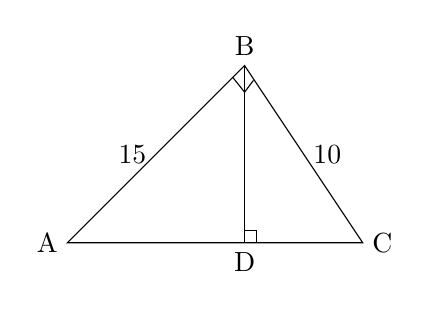
\begin{tikzpicture}[scale=0.75]
\draw (0,0) node[left] {A} -- (3,3) node[above] {B} node[midway,left] {15} -- (5,0) node[right] {C} node[midway, right] {10} -- cycle;
\draw (3,3) -- (3,0) node[below] {D};
\draw (3,0.2) -- (3.2,0.2) -- (3.2,0);
\draw (2.8,2.8) -- (3,2.55) -- (3.15,2.75);
\end{tikzpicture}
\end{center}

If AB = 15 and BC = 10, what is the length of BD?

\bigskip
\textbf{Equation/Strategy:} \hrulefill

\bigskip
\textbf{Solve:}

\vfill
\2 7.5
\2 8
\2 12.5
\2 $\frac{30\sqrt{13}}{13}$
\2 $150-\sqrt{325}$

\midline

\1 What is the ratio of the diagonal of the a cube with a volume of 8 cm$^3$ to the diagonal of a cube with a volume of 64 cm$^3$?

\bigskip
\textbf{Equation/Strategy:}

\bigskip
\textbf{Solve:}

\vfill
\2 $1:8$
\2 $1:4$
\2 $1:2$
\2 $\sqrt{2}:4$
\2 $\sqrt{2}:\sqrt{3}$
\end{outline}
\end{multicols*}
	\section{Transformations} 

\textbf{General Equation:} Let $f(x)$ be a function. Then the function

\[g(x)=a\cdot f(b(x-h))+k\]

is a transformation of $f(x)$ where

\begin{outline}
\1 $a$ is the vertical stretch/compression
\2 If $|a|<1$, then $g$ is a vertical stretch of $f$
\2 If $|a|>1$, then $g$ is a vertical compression of $f$
\2 If $a$ is negative, then $g$ is a reflection of $f$ about the $x-$axis
\1 $b$ is the horizontal stretch
\2 If $|b|<1$, then $g$ is a horizontal stretch of $f$
\2 If $|b|>1$, then $g$ is a horizontal compression of $f$
\2 If $b$ is negative, then $g$ is a reflection of $f$ about the $y-$axis
\1 $h$ is the horizontal shift
\2 If $h>0$, then $g$ is a horizontal shift of $f$ by $h$ units to the right
\2 If $h<0$, then $g$ is a horizontal shift of $f$ by $h$ units to the left
\1 $k$ is the vertical shift
\2 If $k>0$, then $g$ is a vertical shift of $f$ by $k$ units up
\2 If $k<0$, then $g$ is a vertical shift of $f$ by $k$ units down
\end{outline}

\vfill\textbf{Example 1:} Describe the transformation of $f$ by the function $2\cdot g(x)+3=f(x)$.

\vfill\textbf{Example 2:} If $f(3)=-2$, and $g(x)=f(x-2)+3$, what coordinate must be on the graph of $g$?

\vfill\textbf{Example 3:} Let $g(x)=|f(x-1)-2|-3$. What is the vertical shift of $f(x)$ by $g(x)$?

\vfill
\newpage
\begin{multicols*}{2}
\begin{outline}[enumerate]
\centerline{\large MEDIUM}

\1 If $g(x)=|f(x)|$ and $(-x,y)$ is a coordinate of $f(x)$, which of the following is a coordinate of $g(x)$?

\bigskip
\textbf{Equation/Strategy:} \hrulefill

\bigskip
\textbf{Solve:}

\vfill
\2 $(y,x)$
\2 $(x,y)$
\2 $(x,-y)$
\2 $(-x,y)$
\2 $(-x,-y)$

\bigskip
\centerline{\rule{0.4\textwidth}{1pt}}

\bigskip
\1 The graph of $g(x)$ is shown below.

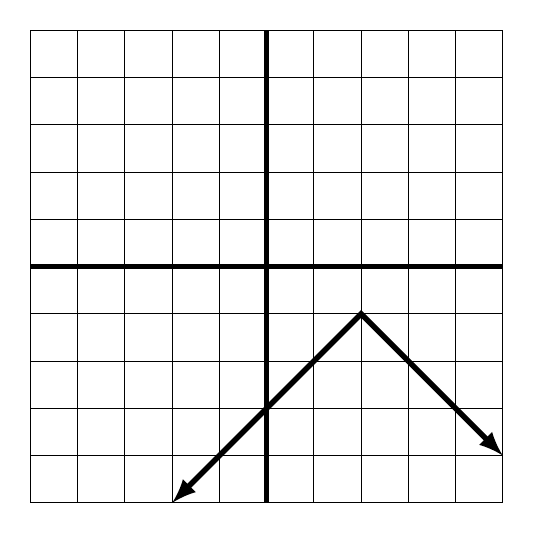
\begin{tikzpicture}[scale=0.6]
\draw (0,0) grid (10,10);
\draw[line width=2pt] (0,5) -- (10,5);
\draw[line width=2pt] (5,0) -- (5,10);
\draw[line width=2pt, latex-latex] (3,0) -- (7,4) -- (10,1);
\end{tikzpicture}

If $g(x)$ is a transformation of $|x|$, which of the following is the equation of $g(x)$?

\bigskip
\textbf{Equation/Strategy:} \hrulefill

\bigskip
\textbf{Solve:}

\vfill
\2 $-|x-2|-1$
\2 $|2-x|-1$
\2 $-|x+2|-1$
\2 $-|x+1|+2$
\2 $-|x-1|+2$

\columnbreak
\centerline{\large ADVANCED}

\1 Which of the following can represent a transformation of the function $f(x)$?

\bigskip
\textbf{Equation/Strategy:} \hrulefill

\bigskip
\textbf{Solve:}

\vfill
\2 $\frac{1}{1/f(x)}$
\2 $f(f^{-1}(f(x))$
\2 $\sqrt[3]{f(x)^3}$
\2 $\sqrt{f(x)^2}$
\2 $f(x\cdot0!)$

\centerline{\rule{0.4\textwidth}{1pt}}

\1 The function $f(x)$ has a coordinate $(m,-n)$. $f(x)$ is shifted $k$ units down and $g$ units right, then reflected across the line $y=x$. Which of the following is the resulting coordinate of the transformation?

\bigskip
\textbf{Equation/Strategy:}

\bigskip
\textbf{Solve:}

\vfill
\2 $(-m-g,n+k)$
\2 $(-n+k,m-g)$
\2 $(m-g,-n+k)$
\2 $(-n-k,m-g)$
\2 $(m-g,-n-k)$
\end{outline}
\end{multicols*}

\chapter{Geometry and Measurement: Part III}
	\section{Coordinate Geometry}

\textbf{General Equation:}

\begin{center}
\begin{multicols}{2}
\setlength{\columnseprule}{0pt}
\textbf{Distance Formula}

\bigskip
$D=\sqrt{(x_2-x_1)^2+(y_2-y_1)^2}$

\textbf{Midpoint Formula}

\bigskip
$P=\left(\frac{x_1+x_2}{2},\frac{y_1+y_2}{2}\right)$
\end{multicols}
\end{center}

\vfill
\begin{enumerate}[labelindent=*,style=multiline,leftmargin=*,label=\textbf{Example \arabic*:}]
\item Points $A$ and $B$ are 5 units apart. If point $A$ is located at $(3,4)$, what is the coordinate of $B$ if it is located in the fourth quadrant?

\vfill\item Points $P$ and $Q$ have coordinates $(3,k)$ and $(n,6)$ respectively. If point $R$ is their midpoint and has a coordinate of $(10, 4)$, what is the value of $n+k$?

\vfill\item What is the area of the triangle formed by the points $(3,1), (9,7)$, and $(3,7)$?
\end{enumerate}

\vfill
\newpage
\begin{multicols*}{2}
\begin{outline}[enumerate]
\medium

\1 The coordinate $(4,6)$ is the midpoint of $(14, 8)$ and which of the following?

\bigskip
\textbf{Equation/Strategy:} \hrulefill

\bigskip
\textbf{Solve:}

\vfill
\2 $(-10,-2)$
\2 $(-4,4)$
\2 $(9,7)$
\2 $(10,2)$
\2 $(24,10)$

\midline

\bigskip
\1 A circle centered at the point $(8,12)$ passes through the point $(12,8)$. What is the length of the circle's diameter?

\bigskip
\textbf{Equation/Strategy:} \hrulefill

\bigskip
\textbf{Solve:}

\vfill
\2 $\sqrt{8}$
\2 $\sqrt{32}$
\2 $2\sqrt{32}$
\2 16
\2 32

\columnbreak
\advanced

\1 The vertices of a triangle have the coordinates $(1,2), (3,4)$, and $(5,6)$. What is the perimeter of the triangle?

\bigskip
\textbf{Equation/Strategy:} \hrulefill

\bigskip
\textbf{Solve:}

\vfill
\2 $\sqrt{32}$
\2 $8\sqrt{2}$
\2 $8+4\sqrt{2}$
\2 8
\2 24

\midline

\1 The vertices of a parallelogram are given by the coordinates $(3,3), (3,m), (1,1),$ and $(1,n)$. If the area of the parallelogram is 12, what is the value of $m+n$?

\bigskip
\textbf{Equation/Strategy:}

\bigskip
\textbf{Solve:}

\vfill
\2 6
\2 12
\2 14
\2 16
\2 18
\end{outline}
\end{multicols*}
	\section{Geometric Visualization}

\textbf{General Equation:}

\vfill
\begin{enumerate}[labelindent=*,style=multiline,leftmargin=*,label=\textbf{Example \arabic*:}]
\item An northward facing arrow is rotated $45^\circ$ counterclockwise, then flipped vertically and horizontally. What direction is the arrow now facing?
\vfill\item Opposite sides of dice have a sum of 7. If John rolls a die three times and the sum of his rolls is 7, what is the sum of the opposite sides of the same three rolls?
\vfill\item A right isosceles triangle with a radius of 2 is rotated about its right angle to form a 3-dimensional solid. What is the volume of the resulting shape?
\end{enumerate}

\vfill
\newpage
\begin{multicols*}{2}
\begin{outline}[enumerate]
\medium

\1 If a circle is cut into regions by three lines, what is the maximum number of regions?

\bigskip
\textbf{Equation/Strategy:} \hrulefill

\bigskip
\textbf{Solve:}

\vfill
\2 
\2 
\2 
\2 
\2 

\midline

\1 A square piece of paper of side length 10 is folded along its diagonal to make a triangle. The triangle is then folded in half down the middle, resulting in another triangle. What is the perimeter of the final triangle?

\bigskip
\textbf{Equation/Strategy:} \hrulefill

\bigskip
\textbf{Solve:}

\vfill
\2 
\2 $10+10\sqrt{2}$
\2 
\2 
\2 

\columnbreak
\advanced

\1 The steering wheel of a boat has 5 spokes, colored red, blue, green, orange, yellow, and purple in that order. If the red spoke faces east when the boat is at rest, what color faces north when the wheel has rotated 1.5 times?

\bigskip
\textbf{Equation/Strategy:} \hrulefill

\bigskip
\textbf{Solve:}

\vfill
\2 
\2 
\2 
\2 
\2 

\midline

\1 A roll of tape has a tube with a diameter of 10 cm and a uniform layer of tape that is 5mm. If the tape has a thickness of 1mm, what is the length of the tape unraveled?

\bigskip
\textbf{Equation/Strategy:}

\bigskip
\textbf{Solve:}

\vfill
\2
\2
\2
\2
\2
\end{outline}
\end{multicols*}

\chapter{Data Analysis, Statistics, and Probability}
	\section{Data Interpretation with Tables}
\textbf{General Equation}

\bigskip
\begin{equationbox}{Data and Tables}
\textbf{Definition:} \textbf{\textit{Data}} is a collection of facts and statistics for reference and analysis. The information from data is gathered and presented in a \textbf{\textit{table}} which arranges categories by columns and rows.
\end{equationbox}

\bigskip
\begin{figure}[h]
\centering
\renewcommand{\arraystretch}{1.5}
\begin{tabular}{cccccccc}
\rowcolor[gray]{.90}
\textbf{\begin{tabular}[c]{@{}c@{}}
Conv/Org\end{tabular}} & \textbf{City} & \textbf{Jan} & \textbf{Feb} & \textbf{Mar} & \textbf{Apr} & \textbf{May} & \textbf{June} \\
Conv & Atlanta & 12.50 & 12.25 & 11.50 & 11.81 & 11.08 & 12.68 \\ \hline
Org & Atlanta & 24.97 & 23.93 & 30.63 & 28.39 & 31.39 & 31.25 \\ \hline
Conv & San Fran & 6.60 & 7.28 & 6.87 & 6.71 & 8.03 & 7.84 \\ \hline
Org & San Fran & 22.00 & 22.00 & 22.00 & 22.00 & 22.00 & 21.96
\end{tabular}
\caption{Prices by city of 1 unit of conventional vs organic produce in 2012}
\end{figure}

\begin{enumerate}[labelindent=*,style=multiline,leftmargin=*,label=\textbf{Example \arabic*:}]
\item According to the table above, which city has the higher average cost of organic produce per unit from January to June?
\vfill\item Approximately what percentage of the average cost of conventional produce of Atlanta is the average cost of organic produce of San Fransisco?
\vfill\item What ratio of months in either city was the cost of 3 units of conventional produce lower than the cost of 1 unit of organic produce?
\end{enumerate}

\vfill
\newpage
\begin{center}
\textbf{\Large Births in Massachusetts in 2012}

\begin{table}[h]
\small\centering
\begin{tabular}{>{\bfseries}{c}|*{12}{c}}
Month & Jan & Feb & Mar & Apr & May & Jun & Jul & Aug & Sept & Oct & Nov & Dec\\\hline
Births & 5,600 & 5,266 & 5,957 & 5,872 & 6,398 & 6,179 & 6,464 & 6,413 & 6,211 & 6,270 & 5,954 & 5,855\\
\end{tabular}
\caption{\small Births in 2012 by month}
\end{table}

\begin{table}[h]
\centering\small
\begin{tabular}{>{\bfseries}{c}|*8{c}}
Day & Sun & Mon & Tues & Wed & Thurs & Fri & Sat\\\hline
Births & 648 & 870 & 1,001 & 836 & 807 & 817 & 621
\end{tabular}
\caption{\small Births in January 2012 by day}
\end{table}
\end{center}

\begin{multicols*}{2}
\begin{outline}[enumerate]
\medium

\1 If there were 72,439 births in Massachusetts in 2012, what ratio of months were the number of births above the average?

\bigskip
\textbf{Equation/Strategy:} \hrulefill

\bigskip
\textbf{Solve:}

\vfill
\2 $1/6$
\2 $1/4$
\2 $1/3$
\2 $1/2$
\2 $2/3$

\midline

\1 Approximately what percentage of babies were born on a weekday in January?

\bigskip
\textbf{Equation/Strategy:} \hrulefill

\bigskip
\textbf{Solve:}

\vfill
\2 $74\%$
\2 $77\%$
\2 $78\%$
\2 $79\%$
\2 $82\%$

\columnbreak
\advanced

\1 Approximately what percentage of the month with the lowest number of births does the difference between that month and the month with the highest number of births represent?

\bigskip
\textbf{Equation/Strategy:} \hrulefill

\bigskip
\textbf{Solve:} 

\vfill
\2 $19\%$
\2 $20\%$
\2 $21\%$
\2 $22\%$
\2 $23\%$

\midline

\1 If there were 5 Sundays, Mondays, and Tuesdays in January of 2012, and only 4 of every other day, which day had the highest average number of births for the month?

\bigskip
\textbf{Equation/Strategy:}

\bigskip
\textbf{Solve:}

\vfill
\2 Monday
\2 Tuesday
\2 Wednesday
\2 Thursday
\2 Friday
\end{outline}
\end{multicols*}
	\section{Data Interpretation with Graphs}
\textbf{General Equation:}

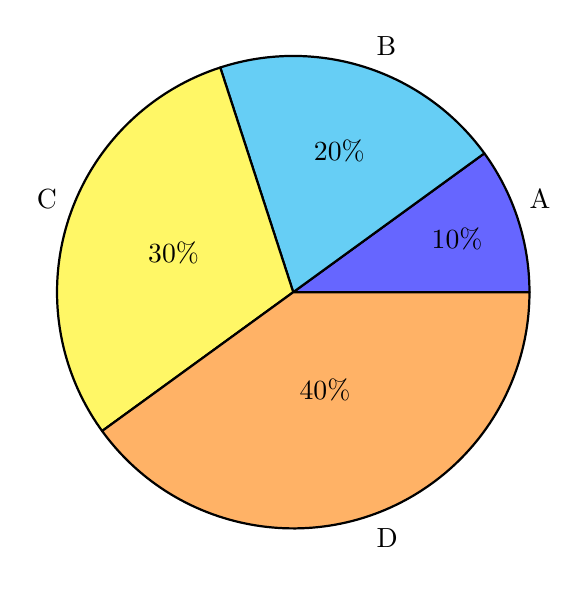
\begin{tikzpicture}
\pie{10/A, 20/B, 30/C, 40/D}
\end{tikzpicture}

\vfill\textbf{Example 1:}

\vfill\textbf{Example 2:}

\vfill\textbf{Example 3:}

\vfill
\newpage
\setlength{\columnseprule}{1pt}
\begin{multicols*}{2}
\begin{outline}[enumerate]
\medium

\1 

\bigskip
\textbf{Equation/Strategy:} \hrulefill

\bigskip
\textbf{Solve:}

\vfill
\2 
\2 
\2 
\2 
\2 

\midline

\1 

\bigskip
\textbf{Equation/Strategy:} \hrulefill

\bigskip
\textbf{Solve:}

\vfill
\2 
\2 
\2 
\2 
\2 

\columnbreak
\advanced

\1 

\bigskip
\textbf{Equation/Strategy:} \hrulefill

\bigskip
\textbf{Solve:}

\vfill
\2 
\2 
\2 
\2 
\2 

\midline

\1 

\bigskip
\textbf{Equation/Strategy:}

\bigskip
\textbf{Solve:}

\vfill
\2
\2
\2
\2
\2
\end{outline}
\end{multicols*}
	\section{Descriptive Statistics: Mean, Median, and Mode}

\textbf{General Equation:}

\begin{itemize}[label=]
\item \textit{Mean} - The sum of all terms in a list, divided by the number of terms
\item \textit{Median} - The middle value in an ordered list
\item \textit{Mode} - The value that occurs most often
\end{itemize}

\begin{enumerate}[labelindent=*,style=multiline,leftmargin=*,label=\textbf{Example \arabic*:}]
\item The average (arithmetic mean) of Sally's previous three tests is 85. If a fourth test boosts her test average up by 2 points, what grade did she receive on her the fourth test?
\vfill\item The median of a set of four numbers is 10. If a large number greater than the other numbers in the set is added to the set, the median becomes 12. What is the value of the second lowest number in the set?
\vfill\item A set of five numbers has a mode of 10. If the average of the set is 25 and the maximum is 50, how many values in the set are equal to the mode?
\end{enumerate}

\vfill
\newpage
\begin{multicols*}{2}
\begin{outline}[enumerate]
\medium

\1 

\bigskip
\textbf{Equation/Strategy:} \hrulefill

\bigskip
\textbf{Solve:}

\vfill
\2 
\2 
\2 
\2 
\2 

\midline

\1 

\bigskip
\textbf{Equation/Strategy:} \hrulefill

\bigskip
\textbf{Solve:}

\vfill
\2 
\2 
\2 
\2 
\2 

\columnbreak
\advanced

\1 

\bigskip
\textbf{Equation/Strategy:} \hrulefill

\bigskip
\textbf{Solve:}

\vfill
\2 
\2 
\2 
\2 
\2 

\midline

\1 

\bigskip
\textbf{Equation/Strategy:}

\bigskip
\textbf{Solve:}

\vfill
\2
\2
\2
\2
\2
\end{outline}
\end{multicols*}
	\section{Probability}

\textbf{General Equation:}

\begin{center}
\renewcommand{\columnseprule}{0pt}
\begin{multicols}{2}
$P_{A\mbox{ and }B}=P_A\cdot P_B$

$P_{A\mbox{ or }B}=P_A+P_B-P_{A\mbox{ and }B}$
\end{multicols}
\end{center}

\begin{enumerate}[labelindent=*,style=multiline,leftmargin=*,label=\textbf{Example \arabic*:}]
\item Liang is playing a game with a standard deck of cards. He wants the first card he picks up to be either a red card or a face card (Jack, Queen, or King). What is the probability he will choose either a red card or a face card?
\vfill\item
\vfill\item
\end{enumerate}

\vfill
\newpage
\begin{multicols*}{2}
\begin{outline}[enumerate]
\medium

\1 

\bigskip
\textbf{Equation/Strategy:} \hrulefill

\bigskip
\textbf{Solve:}

\vfill
\2 
\2 
\2 
\2 
\2 

\midline

\1 

\bigskip
\textbf{Equation/Strategy:} \hrulefill

\bigskip
\textbf{Solve:}

\vfill
\2 
\2 
\2 
\2 
\2 

\columnbreak
\advanced

\1 

\bigskip
\textbf{Equation/Strategy:} \hrulefill

\bigskip
\textbf{Solve:}

\vfill
\2 
\2 
\2 
\2 
\2 

\midline

\1 

\bigskip
\textbf{Equation/Strategy:}

\bigskip
\textbf{Solve:}

\vfill
\2
\2
\2
\2
\2
\end{outline}
\end{multicols*}

\part{SAT Verbal}

\chapter{The Six Most Frequently Missed Errors on SAT Writing Multiple Choice: Strategies for Sentence Improvements and Sentence Errors}
	\section{The Six Most Frequently Missed Errors on SAT Writing Multiple Choice: Strategies for Sentence Improvements and Sentence Errors}

\subsection{SAT Worksheet: Warm-Up}

\textit{Directions: Please order the following types of questions on the SAT writing section from 1 to 4 where 1 is the most difficult type of question for you and 4 is the least difficult types of questions for you.Then, do the example of Improving Sentences and Sentence Errors on the sheet.}

\bigskip
\underline{\hspace{2in}} \textbf{Improving Sentences}

\bigskip
The travel guide is useful because it covers not just reviews and photos, \ul{ but also tells you what and how to get to various destinations.}

\begin{enumerate}[label=(\Alph*)]
\item{but also tells you what and how to get to various destinations.}
\item{but also they gives ways of getting to various destinations.}
\item{but also advice of what and how to get to various destinations.}
\item{but also tells you what to do and how to get to various destinations.}
\item{and also tells you what to do and how to get to various destinations.}
\end{enumerate}

\bigskip
\underline{\hspace{2in}} \textbf{Sentence Errors}

\bigskip
\begin{inparaenum}[A]
Jean Rhys, \tfrac{whose}{\item} Dominican background \tfrac{has influenced}{\item} her writing, \tfrac{describes}{\item} many details of life in the Caribbean Islands \tfrac{vividly}{\item} in her novels and short stories. \tfrac{No Error}{\item}
\end{inparaenum}

\bigskip
\underline{\hspace{2in}} \textbf{Paragraph Improvements}

\bigskip
\underline{\hspace{2in}} \textbf{Essay}
	\section{About the SAT Writing Section}

\begin{spacing}{1.5}
Your score on the SAT writing section is dependent upon your performance in three sections, two multiple choice sections and one essay section. The essay section is the \shortline on the SAT and consists of \shortline essay assignment. You will have \shortline minutes to complete the essay. We will focus on the essay in a later chapter. 

\bigskip
\sloppy In this section of the SAT manual, we will concentrate on the multiple choice sections. There are two multiple choice sections, one with \shortline questions to be completed in \shortline minutes and one with \shortline questions to be completed in \shortline minutes.
\end{spacing}
	\section{Types of Writing Multiple Choice Questions}

\begin{enumerate}
\item{The first type of writing multiple choice questions is \hrulefill}
\begin{itemize}
\item{In this type of question, one part of a sentence will be underlined and you will be asked to pick the version of the underlined part of the sentence.}
\item{This type of question is found in both the 25-minute and the 10-minute multiple choice sections.}
\end{itemize}


\item{The second type of writing multiple choice questions is \hrulefill}
\begin{itemize}
\item{In this type of question, you will be asked to identify whether or not there is an error
in the sentence given, and if so, circle the location of the error. You will not be asked
to correct the error on the SAT.}
\item{This type of question is found in the 25-minute multiple choice section only.}
\end{itemize} 

\item{The last type of writing multiple choice questions is \hrulefill}
\begin{itemize}
\item{Approximately half of the questions are sentence improvement and sentence revision.}
\item{The other questions are paragraph or essay structure and logic questions.}
\item{There are a total of 6 paragraph improvement questions on the SAT, all in the 25-minute section.}
\end{itemize}

\end{enumerate}
	\section{Mastering Sentence Improvement and Sentence Error Questions}

The SAT Writing multiple choice section may seem intimidating at rst, as there is a lot of reading (particularly for the sentence improvement and paragraph improvement questions) as well as many questions to answer in each section. However, the SAT tests standard English grammar, which means that if students learn a handful of grammar rules--particularly the ones featured in this
section--then they will be able to complete many questions in the SAT writing section carefully.

\bigskip
Remember, the SATs tests \textbf{proper grammar} as well \textbf{conciseness}. How we talk is not always
grammatically correct, and therefore not the correct answer on the SATs. Be cautious of this,
particularly on the later (more difficult) questions. We will address the issue of conciseness in the
next chapter, but usually if you have narrowed a question down to two or three answer choices
that are each grammatically correct, the correct answer is the shortest answer choice.

\bigskip
Verb tense, pronouns, misplaced modiers, parallelism, faulty conjunctions, and idioms are the six
most commonly missed errors on the SAT Writing multiplce choice section. By reviewing these
grammar concepts as well as completing the practice problems, you should be able to answer SAT
Writing multiple choice questions more accurately.
	\section{Verb Tense}

Verbs must agree with their subject in number. Many errors on the SAT writing section is related to subject-verb agreement and verb tense.
\subsection{Subject-Verb Agreement}

\begin{itemize}
\item{This is manageable when sentences are straightforward.}
\item{For example, fill in the following blanks: He \hrulefill smart. They \hrulefill smart.}
\item{To make the questions more difficult, the SATs will separate the subject and the verb with prepositional phrases or descriptions
with commas. An SAT question may also put
the verb before the subject.}
\item{For example: Stephen for more than two weeks \hrulefill happy because of his most recent grades. To solve
this type of question, identify the subject and cross out prepositional phrase. Then, identify
the correct verb form.}

\bigskip
Looking at it like this indicates that the subject is ``Stephen'' and so ``is'' is correct form of
the verb.

\item{For example: The group, consisting of two adults and five children, \hrulefill camping this weekend. To solve this type of question, identify the subject and cross out description (between the commas). Then, identify the correct verb form.}

\bigskip
The subject is ``the group'' and so ''is'' is correct form of the verb.

\item{For example: Running \hrulefill the girls' favorite sport. To solve this type of question, rearrange the sentence so that the subject comes before the verb. Then, identify the correct verb form.}

\bigskip
The sentence is re-arranged as ``'The girls' favorite sport \underline{\hspace{2in}} running.'' Therefore, the correct verb form is ``'is.''
\end{itemize}


	\section{SAT Worksheet: SAT Writing Multiple Choice Practice with Subject-Verb Agreement}

\textit{Directions: In the following sentences, box the subject and circle the verb that agrees with the subject.}

\begin{enumerate}
\item{I never \textbf{ have or has} long fingernails because I bit them.}


\item{Finding happiness from multiple sources \textbf{is or are} important.}


\item{The dolls in the storage closet \textbf{sits or sit} on the shelf.}


\item{Plastic engineering, a booming field in many countries, \textbf{have or has} many important applications.}


\item{Reading papers \textbf{is or are} the best part of my day.}


\item{The trails, which I climb daily, \textbf{widen or widen}s towards the end.}

\end{enumerate}

\subsection{Using the Correct Verb Tense}

Knowing when to use different verb tenses are important for SATs. Sometimes, you can look for
clues based on other part of the sentence. For example, ``Based on his previous experiences, Jared
decides/decided to pursue a career in education.''

\bigskip
It can be difficult to determine if something should be simple present, past, or future versus present
perfect, past perfect, and future perfect. For example, when should you use ``waited'' versus ``had
waited''?

\begin{itemize}
\item{We use the simple tenses when there is one year or date. Select the correct verb tense in the following sentence: World War II
began/had begun in 1939.}
\item{We use past perfect when an action has started and it is interrupted by another action (past
tense). Select the correct verb tense in the following sentence: World War II occurred/had occurred for two years before the United
States entered it in 1941.}
\item{We use present perfect for an action that began in the past and continues to the persent.
Explain the difference between the following sentences:}

\begin{enumerate}
\item{Scott had lived in New York for five years before he decided to move.}
\item{Scott has lived in New York for five years, although he is currently considering moving.}
\end{enumerate}

The first sentence \hrulefill whereas the second \hrulefill.

\item A note about SAT grammar: ``The conditional (would) is used for hypothetical situations. The basic formula is ``\textit{If \ldots were \ldots would''.} Select the correct verb tense in the following sentence: If I was/were to win the lottery, then I will/would travel around the world.

\end{itemize}

\subsection{Sample SAT Practice Questions}

\begin{enumerate}
\item \begin{inparaenum}[A]
The janitors \tfrac{are}{\item} \tfrac{requiring}{\item} to mop the floors, \tfrac{wipe}{\item} the windows, and clean the chalkboard \tfrac{daily}{\item}. \tfrac{No Error}{\item}
\end{inparaenum}

\item \begin{inparaenum}[A]
The teachers, \tfrac{iinspired by}{\item} the novel \tfrac{pedagogical}{\item} techniques they learned at the conference, \tfrac{pledge to}{\item} utilize these methods to improve their \tfrac{teaching}{\item}. \tfrac{No Error}{\item} 
\end{inparaenum}

\end{enumerate}
	\section{Pronouns}
Some common pronoun rules tested on the SAT Writing Section are agreement, unclear pronouns,
and inconsistent point of view.

\subsection{Agreement with the Antecedent}
\begin{enumerate}
\item{What is an antecedent?} \hrulefill
\item{Circle the antecedent and box the pronoun in the following sentence: Kenna the dog plays
with her favorite chew toys daily.}

\end{enumerate} 

\subsection{Unclear Pronouns}
Pronouns need to be clear regarding who or what they are referring to.
\begin{enumerate}
\item Emily and Kate are going to her house today. Why is this sentence incorrect?

\hrulefill
\item She is going to teach them today. Why is this sentence incorrect?

\hrulefill
\item The amusement park rides are full of mice, therefore we will avoid them. Why is this sentence
incorrect?

\hrulefill
\item Write a possible correction to the following sentence: The amusement park rides are full of
mice, therefore we will avoid them.

\hrulefill
\end{enumerate}

\subsection{Consistent Point of View}
Each sentence or paragraph needs to have the same point of view. For example, the following
sentence is incorrect: 

\bigskip
If one wants to go to the store, then I recommend that you find a driver.

\begin{itemize}
\item{\textbf{Correct:} If you want to want to go to the store, then I recommend that you find a driver.}
\item{\textbf{Another correct version of this sentence is,} If one wants to go to the store, I recommend that
one finds a driver.}
\item{Circle the following choice that makes the sentence correct: You/one should never complain, even when one is given a difficult task.}
\item{Why is the answer that you circled correct?} \hrulefill
\end{itemize}

\subsection{Sample SAT Practice Questions}

\begin{enumerate}

\item \begin{inparaenum}[A]
As nervous as \tfrac{her}{\item} mom \tfrac{was}{\item}, the second grader was determined \tfrac{to walk to}{\item} the bus stop by \tfrac{herself}{\item}.\tfrac{No Error}{\item}
\end{inparaenum}

\item \begin{inparaenum}[A]
If I \tfrac{was}{\item} to invent a time machine, then \tfrac{I}{\item} would go back in time to the period around the Revolutionary War and learn \tfrac{firsthand}{\item} what it \tfrac{was}{\item} like to fight for freedom. \tfrac{No Error}{\item}
\end{inparaenum}

\end{enumerate}
	\section{Misplaced Modifiers}
A modifier is a group of word describing a noun or pronoun. In proper grammar (a.k.a. on the SATs), modifiers need to be next to what they are describing.


For example,

\bigskip
\begin{itemize}
\item{\textbf{Incorrect:} Running down the street, the trash can was in Lauren's way.}
\item{The problem here is that we know Lauren is running down the street but the sentence implies that the trash can is running because trash can is what comes directly after the modifier.}
\item{\textbf{Better but still wrong:} While running down the street, Lauren's way was blocked by a trash can. In this case Lauren's way appears to be running down the street.}
\item{\textbf{Correct: While running down the street, Lauren had a trash can in her way.}}
\item{Finally, we have Lauren, the subject, being modified and the modifier next to the subject.}
\end{itemize} 

\vfill
\subsection{\sloppy SAT Worksheet: SAT Writing Multiple Choice Practice with Modifiers}
\textit{Directions: Underline the modifier and then circle what the modifier is modifying. If the modifier is not next to what it is modifying, re-write the sentence so that the modifier is next to what it is modifying.}

\bigskip
\begin{enumerate}
\item{Since he is a gentleman, Adam is always willing to help others.}

Re-write: \hrulefill

\bigskip
\hrulefill

\vfill\item{Having come down lightly throughout the morning, Sarah thought that she would be able to move her car through the snow.}

Re-write: \hrulefill

\bigskip
\hrulefill

\vfill\item{Full of lights, we were impressed with the holiday tree.}

Re-write: \hrulefill

\bigskip
\hrulefill

\end{enumerate}

\newpage
\subsection{Practice SAT Questions}

\begin{enumerate}
\begin{spacing}{1.5}
\item \begin{inparaenum}[A]
\tfrac{By this}{\item} time next year,  \tfrac{we will}{\item} have acquired ten new accounts and \tfrac{have}{\item} opened two new offices \tfrac{abroad}{\item}. \tfrac{No Error}{\item}
\end{inparaenum}
\end{spacing}

\item \ul{Dangling from the trees, we were frightened by the monkeys that tried to steal our sunglasses.} 

\begin{enumerate}[label=(\Alph*)]
\item Dangling from the trees, we were frightened by the monkeys that tried to steal our sunglasses. 
\item Dangling from the trees, the monkeys tried to steal our sunglasses, an action which frightened us. 
\item The monkeys frightened us when they tried stealing our sunglasses dangling from trees. 
\item Dangling from trees, the monkeys frightened us trying to steal our sunglasses. 
\item The monkeys, dangling from the trees, frightened us when they tried to steal our sunglasses. 
\end{enumerate}

\end{enumerate}

	\section{Parallelism}

Clauses within a sentence must have the same phrasing (parts of speech or verb tenses). This
frequently happens to items in a list. Parallelism can also apply to the paragraph improvement
section where consecutive sentences have similar structure.

\bigskip
For example,
\begin{enumerate}

\item Emily likes soccer, hockey, and going to parties. 

What is wrong with this sentence? 

\hrulefill

Write a correct version of the sentence:

\hrulefill
\item When at college, Emily likes to go to soccer games, football games, and play frisbee. 

What
is wrong with this sentence?

\hrulefill

Write a correct version of the sentence:

\hrulefill
\item Kelly likes to go to the mall, but riding on the mall's elevators scares her. 

What is incorrect about this sentence?

\hrulefill

Write a correct version of the sentence:

\hrulefill
\end{enumerate}

\subsection{Practice SAT Questions}

\begin{enumerate}
\item \ul{The boy spoke three languages fluently: French, Spanish, and Russian.}

\begin{enumerate}[label=(\Alph*)]
\item The boy spoke three languages fluently: French, Spanish, and Russian. 
\item The fluent boy spoke three languages: French, Spanish, and Russian.
\item The boy spoke French, Spanish, and Russian fluently.
\item The boy spoke three languages fluently French, Spanish, and Russian. 
\item The boy was able to speak three languages fluently: French, Spanish, and Russian. 
\end{enumerate}

\begin{spacing}{1.5}
\item \begin{inparaenum}[A]
Mary \tfrac{was}{\item} walking \tfrac{towards the bus}{\item} when she \tfrac{decides}{\item} that she would \tfrac{prefer to}{\item} take a cab instead. \tfrac{No Error}{\item}
\end{inparaenum}
\end{spacing}
\end{enumerate}
	\section{Faulty Comparisons}

Items being compared must have the same identity. For example, a dog can not be compared to another dog's toys. While this might sound easy, it isn't always easy because our brain is used to making the correct comparison even if it is written incorrectly on the page.

For example,

\begin{enumerate}
\item Spot is better than Ziggy's toys.

\begin{itemize}
\item The sentence is trying to compare Spot and Ziggy or Spot's toys and Ziggy's toys.
\item The sentence is actually comparing Spot and Ziggy's toys.
\item This sentence can be corrected at least two different ways. Spot's toys are better
than Ziggy's toys. OR Spot's toys are better than Ziggy's.
\end{itemize}

\item Paul's pet rock is larger than Jim.

\begin{itemize}
\item What two things is the sentence trying to compare? \hrulefill
\item What two things is the sentence actually comparing? \hrulefill
\item Re-write the sentence so that it is grammatically correct (Note: there are at least two
ways to do this.): \hrulefill
\end{itemize}
\end{enumerate}

\subsection{SAT Practice Questions}

\begin{enumerate}

\begin{spacing}{1.5}
\item \begin{inparaenum}[A]
J.K. Rowling’s books \tfrac{have inspired}{\item} millions with stories \tfrac{of}{\item} good triumphing over evil and the power of friendship, \tfrac{whereas}{\item} the new \tfrac{author}{\item} has not. \tfrac{No Error}{\item}
\end{inparaenum}

\item \begin{inparaenum}[A]
The cameraman  \tfrac{told}{\item} the celebrity that  \tfrac{he}{\item} should position  \tfrac{himself}{\item} \tfrac{closer to}{\item} the camera. \tfrac{No Error}{\item}
\end{inparaenum}
\end{spacing}
\end{enumerate}
	\section{Word Choice}
The errors can be wrong words. These can be in the form of

\begin{itemize}
\item{idioms. What are idioms?} \hrulefill

Fill in the correct prepostion(s) after the verb:

\begin{enumerate}
\item to agree \hrulefill
\item to go ahead \hrulefill
\item to manage \hrulefill
\item to prefer \hrulefill
\item to prepare \hrulefill
\item to rebel \hrulefill
\item to rely \hrulefill
\item to be satisfied \hrulefill
\item to want \hrulefill
\end{enumerate}

\item{commonly confused words. For example, when do you use the word ``affect'' instead of ``effect''? } \hrulefill

\item{incorrect word choice.} 

Fill in the correct word(s) in the phrase. Then, write a sentence that uses the phrase correctly. The first one has been done as an example:

\begin{enumerate}
\item as \ldots \ul{as}
Sentence: The basketball player was as tall as the net.

 \item decide between \ldots \hrulefill 

\item either \dots \hrulefill
Sentence:

\item neither \ldots \hrulefill
Sentence:

\item not only \ldots \hrulefill
Sentence:

\item rather \ldots \hrulefill
Sentence:

\end{enumerate}
\end{itemize} 

\subsection{Practice SAT Questions}

\begin{enumerate}
\item \begin{inparaenum}[A]
The student \tfrac{wanted}{\item} \tfrac{both to}{\item} remain in Boston  \tfrac{or}{\item} move  \tfrac{to the West Coast}{\item} after graduation. \tfrac{No Error}{\item}
\end{inparaenum}

\item \begin{inparaenum}[A]
Over thirty million people were \tfrac{effected by}{\item} the snowstorm, and \tfrac{to this day}{\item}, many people are frightened when the \tfrac{news says}{\item} that there is a \tfrac{possibility of snow}{\item}. \tfrac{No Error}{\item}
\end{inparaenum}

\item \begin{inparaenum}[A]
\tfrac{After}{\item} waiting an hour for \tfrac{her}{\item} friend, the woman \tfrac{finally}{\item} arrived \tfrac{in}{\item} the theater. \tfrac{No Error}{\item}
\end{inparaenum}

\end{enumerate}




	\section{Other Common Errors}

The following is a list of other common errors that you will discuss as a class. Then, circle and correct the error:
\begin{itemize}
 \item{Adverbs vs. Adjectives:} \hrulefill
 She worked diligent to ensure that the assignment was completed in a timely manner. 
 
\item{Comparatives vs. Superlatives:} \hrulefill
\item{Sentence Fragments:} \hrulefill
\item{Redundancy:} \hrulefill
\item{Run-ons:} \hrulefill
\item{Passive Voice: } \hrulefill

\end{itemize} 

\chapter{Sentence Improvements}
	\section{SAT Worksheet: Warm-Up}

Are you having trouble remembering what types of errors are tested in the SAT Writing section?
Try this mnemonic device:

The most commonly tested and missed grammar points can be seen below. When you are answers sentence error or improvement questions, BE A CYCLOPS and always be keep one eye open for these most commonly missed grammar points. If you have already heard the BE A CYCLOPS mnemonic from another section, close your eyes and identify the grammar point that each letter refers to. Then, complete the exercise on the next page. 

\bigskip
\textbf{B is for ``being":} The word ``being" is commonly heard in speech but does not usually make for the best sentences.

\bigskip
\textbf{E is for agrEEmEnt:} Identify the subject and the verb that is associated with the subject. The verb needs to match the subject in number and gender. This means that the subject and the main verb need to be both singular or both plural. 

\bigskip

\bigskip
\textbf{A is for awful verb tense:} Check when the action is happening and then if the given verb tense can be used to describe the time period that the action is happening. 

\bigskip

\bigskip
\textbf{C is for clause (aka commas towards the beginning of the sentence):} Clauses at the beginning of sentences have a description, then a comma, then more words. The description must be describing the first word after the comma. 

\bigskip
\textbf{Y is for you, me, and other pronouns:} If ``you" is not in the underlined section, then it must be paired with ``you" in the underlined section. If ``one" or ``someone" is not in the underlined section, then it must be paired with you in the underlined section. Also, make sure that pronouns like ``it" or ``they" clearly refer to the subject of the sentence. 

\bigskip
\textbf{C if for contrasts and other conjunction/connectors:} Words like ``and" are used to add another idea, however, words like ``but" are used to show differences between things. 

\bigskip
\textbf{L is for list:} If there is a list, all of the words must be the same part of speech and the same verb tense. 

\bigskip
\textbf{O is for ``of" and commas that might separate the subject and the verb:} The verb ending is dependent on the singularity or plurality of the subject.

\bigskip
\textbf{P is for preposition:} Make sure the preposition matches the word before it. To combat this, learn your idioms!

\bigskip
\textbf{S is for short:} Is the sentence as short as it can be without changing the meaning? 

\vfill

\newpage
\textit{Directions: Write 5 sentence error questions from any five different categories in the list above. At least one should have no error. Then, switch with someone in the class so that they can solve your questions.}

\begin{enumerate}
\item
\vfill\item
\vfill\item
\vfill\item
\vfill\item\vfill
\end{enumerate}
\vfill
	\section{Identify the Error or Errors in the Original Sentence}
If you can identify the error or errors in the original sentence before looking at the answer choicaes. This can help you identify if there is an error and if so, to determine which changes need to be made in the correct answer choice. 

For example, try to identify the error in the following sentences:

It is extremely advantageous if you can identify the error or errors in the original sentence before looking at the answer choices and then think of possible corrections. These can help you to 1) Eliminate answer choice ``A" as the best sentence and 2) eliminate incorrect answer choices with the same error as the original sentence quickly. 

\bigskip
\textit{Directions: Determine if the sentences below have an error in the underlined region and, if so, circle it. Write the type of error on the first line and a sample correction on the second line. If you don't that there is an error, write ``No error" as the error type and move to the next sentence. The first question has been done for you.}

\begin{spacing}{1.5}
\begin{enumerate}
\item The Boston Common is \ul{ older than it but still just as well-maintained as Central Park}.

\bigskip
\textbf{Type of error(s):} \ul{unclear pronoun, not concise}

\textbf{Sample correction:} \ul{older than but still just as well-maintained as Central Park.}

\bigskip
\item While most people detest high prices \ul{for food items, but organic food sells well despite the increased cost.}

\bigskip
\textbf{Type of error(s):} \hrulefill

\textbf{Sample correction:} \hrulefill

\item With determination and diligence, anyone can achieve a high score on the SAT test. 

\bigskip
\textbf{Type of error(s):} \hrulefill

\textbf{Sample correction:} \hrulefill

\bigskip
\item The movie \ul{featured many well-respected actors and was winning many awards for} acting, directing, producing, and writing.

\bigskip
\textbf{Type of error(s):} \hrulefill

\textbf{Sample correction:} \hrulefill

\bigskip
\item \ul{Many educators believe that technology of the sort that} helps monitor student progress and deliever feedback to parents could be helpful in increasing test performance. 

\bigskip
\textbf{Type of error(s):} \hrulefill

\textbf{Sample correction:} \hrulefill

\item After waiting an hour for her friend, the woman finally \ul{arrived in the theater donning a red dress.}

\bigskip
\textbf{Type of error(s):} \hrulefill

\textbf{Sample correction:} \hrulefill

\item Overjoyed that he was accepted his first choice college, \ul{Stephen is currently being slightly ridiculous.}

\bigskip
\textbf{Type of error(s):} \hrulefill

\textbf{Sample correction:} \hrulefill

\item \ul{Many people think that Americans take the right to vote for granted, and I think that it is the right of Americans to not exercise their right to vote.}

\bigskip
\textbf{Type of error(s):} \hrulefill

\textbf{Sample correction:} \hrulefill

\item The bank robbers threatened the tellers by waving their guns, one of the criminals held a teller hostage until the police arrived. 

\bigskip
\textbf{Type of error(s):} \hrulefill

\textbf{Sample correction:} \hrulefill

\item After a major political event such as September 11th, the president will address the nation, with his purpose being to inform and comfort the public.

\bigskip
\textbf{Type of error(s):} \hrulefill

\textbf{Sample correction:} \hrulefill

\item Mary's secret, the whereabouts of the items that had been missing for weeks, \ul{were more compelling than Jeff's.}

\bigskip
\textbf{Type of error(s):} \hrulefill

\textbf{Sample correction:} \hrulefill
\end{enumerate}
\end{spacing}
	\section{Strategy: Eliminate Incorrect Answers then Find the Most Concise Answer}

On sentence improvements, the correct answer will be grammatically correct. Therefore, before
you see if an answer choice makes sense in the original sentence, determine if it is grammatically
correct. If not, then you can eliminate this right away.

In SAT sentence improvement problems, you should try to eliminate the 2-3 answer choices that are grammatically incorrect so that you are left with 2-3 other answer choices. The SAT sentence improvement section is looking for the "best" sentence, one that is concise and precise. In SAT world, this translates to the sentence that is not only grammatically correct AND concise. How does the SAT measure ``conciseness''? By length.

\bigskip
Therefore, the answer choice that you are looking for is grammatically correct and short without changing the meaning of the original sentence. The latter part means that it can not be so short that it is missing a key part of the original sentence,
but this is not usually an issue on sentence improvement problems.

\bigskip
Find the shortest answer. Then, check if it preserves the original meaning of the sentence by reading this answer choice in place of the underlined part of the original sentence. If so, this answer choice is the correct answer, so you should mark it.

\bigskip
\textit{Directions: Eliminate the answer choices that are grammatically incorrect for the following sentences. After you have eliminated an answer choice, write why it was incorrect on the line. Then, determine the correct answer using the strategy presented above. The first one has been done for you.}


<<<<<<< HEAD
\begin{enumerate}
\item The Boston Common is \ul{ older than it but still just as well-maintained as Central Park}.

\begin{enumerate}[label=(\Alph*)]
=======
\item The Boston Common is \ul{older than it but still just as well-maintained as Central Park}.
>>>>>>> 70cbfedac09602262caef6f421f9691f9f5a5fc2

\begin{enumerate}[label=(\Alph*)]
\item older than it but still just as well-maintained as Central Park 

  \ul{Eliminate because of ambiguous pronoun}
  
\item older than Central Park but just as well-maintained. 

\textbf{\ul{Correct. It is grammatically correct and the most concise.}}

\item  older than Central Park; it is just as well-maintained.   

  \ul{Eliminate because of ambiguous pronoun}
  
\item older and it is just as well-maintained as Central Park. 

\textbf{\ul{Grammatically correct but not as concise as (B).}}

\item just as comfortable as Central Park and it is older than it. \ul{Eliminate because of ambiguous pronoun}

\end{enumerate}

\bigskip
\item While most people detest high prices \ul{for food items, but organic food sells well despite the increased cost.}

\bigskip
\begin{enumerate}[label=(\Alph*)]
\item for food items, but organic food sells well despite the increased cost. \hrulefill
 
\item for food items, organic food sells well despite the increased cost. \hrulefill
 
\item for food items, many people still purchase organic food despite the increased cost. \hrulefill

\item for food items, despite the increased cost, organic food sells well. \hrulefill
 
\item for food, but organic food sells well despite the increased cost. \hrulefill

\end{enumerate}

\bigskip
\item \ul{With determination and diligence, anyone can achieve a high score on the SAT test.}

\bigskip
\begin{enumerate}[label=(\Alph*)]

\item With determination and diligence, anyone can achieve a high score on the SAT test. \hrulefill
\item With determination and diligence, anyone is achieving a high score on the SAT test.\hrulefill
\item Anyone full of determination and diligence achieves a high score on the SAT test.\hrulefill
\item Determination and diligence can help anyone who wants to achieve a high score on the SAT test. \hrulefill
\item Anyone can achieve a high score on the SAT test with determination and diligence.\hrulefill
\end{enumerate}

\bigskip
\item The movie \ul{featured many well-respected actors and was winning many awards for} acting, directing, producing, and writing. 

\bigskip
\begin{enumerate}[label=(\Alph*)]
\item featured many well-respected actors and was winning many awards for \hrulefill
\item featured many well-respected actors, was winning many awards for\hrulefill
\item featured many actors that were well-respected and won many awards for \hrulefill
\item had featured many well-respected actors and won many awards for\hrulefill
\item featured many well-respected actors and won many awards for \hrulefill
\end{enumerate}

\bigskip
\item \ul{Many educators believe that technology of the sort that} helps monitor student progress and deliever feedback to parents could be helpful in increasing test performance. 

\bigskip
\begin{enumerate}[label=(\Alph*)]
\item Many educators believe that technology of the sort that \hrulefill
\item Many educators believe technology that \hrulefill
\item Many educators believe that technology which \hrulefill
\item A group of educators believe that technology that \hrulefill
\item Many educators believe that technology that \hrulefill
\end{enumerate}

\bigskip
\item After waiting an hour for her friend, the woman finally \ul{arrived in the theater donning a red dress.}

\bigskip
\begin{enumerate}[label=(\Alph*)]
\item arrived in the theater donning a red dress.\hrulefill
\item donned a red dress and arrived in the theater. \hrulefill
\item arrived in the theater and donned a red dress. \hrulefill
\item arrived in the theater wearing a red dress.\hrulefill
\item arrived at the theater donning a red dress.\hrulefill
\end{enumerate}

\bigskip
\item Overjoyed that he was accepted his first choice college, \ul{Stephen is currently being slightly ridiculous.}

\bigskip
\begin{enumerate}[label=(\Alph*)]
\item Stephen is currently being slightly ridiculous \hrulefill
\item Stephen is currently slightly ridiculous\hrulefill
\item Stephen is acting slightly ridiculous.\hrulefill
\item slightly rediculous Stephen is being. \hrulefill
\item currently Stephen is being slightly ridiculous.\hrulefill
\end{enumerate}

\bigskip
\item \ul{Many people think that Americans take the right to vote for granted, and I think that it is the right of Americans to not exercise their right to vote.}

\bigskip
\begin{enumerate}[label=(\Alph*)]
\item Many people think that Americans take the right to vote for granted, and I think that it is the right of Americans to not exercise their right to vote. \hrulefill
\item Americans take the right to vote for granted according to many people, and I think that it is the right of Americans to not exercise their right to vote.\hrulefill
\item Many people think that Americans had taken the right to vote for granted, and I think that it is has been the right of Americans to not exercise their right to vote. \hrulefill
\item Many people think that Americans take the right to vote for granted, but I think that it is the right of Americans to not exercise their right to vote.\hrulefill
\item Americans take the right to vote for granted, yet it is the right of Americans to not exercise their right to vote.\hrulefill
\end{enumerate}

\bigskip
\item The bank robbers \ul{threatened the tellers by waving their guns, one of the criminals held a teller hostage} until the police arrived. 

\bigskip
\begin{enumerate}[label=(\Alph*)]
\item threatened the tellers by waving their guns, one of the criminals held a teller hostage \hrulefill
\item threatened the tellers by waving their guns. One of the criminals held a teller hostage\hrulefill
\item threatened the tellers by waving their guns; one of the criminals held a teller hostage\hrulefill
\item waving their guns to threat the tellers. One of the criminals held a teller hostage\hrulefill
\item waved their guns to threat the tellers; one of the criminals held a teller hostage\hrulefill
\end{enumerate}

\bigskip
\item After a major political event such as September 11th, \ul{the president will address the nation, with his purpose being to inform and comfort the public.}

\bigskip
\begin{enumerate}[label=(\Alph*)]
\item the president will address the nation, with his purpose being to inform and comfort the public. \hrulefill
\item the president will address the nation so that he can inform and comfort the public.\hrulefill
\item the president will address the nation to inform and comfort the public.\hrulefill
\item the president addresses the nation, with his purpose being to inform and comfort the public.\hrulefill
\item the president will address the nation, with the purpose to inform and comfort the public.\hrulefill
\end{enumerate}

\bigskip
\item Mary's secret, the whereabouts of the items that had been missing for weeks, \ul{were more compelling than Jeff's.}

\bigskip
\begin{enumerate}[label=(\Alph*)]
\item were more compelling than Jeff's. \hrulefill
\item were more compelling than Jeff's secret. \hrulefill
\item was more compelling than what Jeff said. \hrulefill
\item were more compelled than Jeff's. \hrulefill
\item was more compelling than Jeff's.\hrulefill
\end{enumerate}

\end{enumerate}

	\section{Practice with SAT Sentence Errors and Improvements}

\subsection{SAT Warm Up Sheet}

\textit{Directions: Use the strategies that we have discussed to answer the following Sentence Improvement and Error SAT Questions.}

\begin{enumerate}
\item Dangling from the trees, \ul{we were frightened by the monkeys that tried to steal our sunglasses.}

\begin{enumerate}[label=(\Alph*)]
\item we were frightened by the monkeys that tried to steal our sunglasses.
\item we had been frightened by the monkeys that tried to steal our sunglasses.
\item the monkeys frightened us because they tried to steal our sunglasses.
\item we were frightened by the monkeys who had tried to steal our sunglasses.
\item the monkeys that tried to steal our sunglasses frightened us. 
\end{enumerate}
\end{enumerate}

In SAT sentence improvement problems, you should try to eliminate the 2-3 answer choices that are grammatically incorrect so that you are left with 2-3 other answer choices. The SAT sentence improvement section is looking for the ``best'' sentence, one that is concise and precise. In SAT world, this translates to the sentence that is not only grammatically correct AND concise. How does the SAT measure ``conciseness''? By length.

\bigskip
Therefore, the answer choice that you are looking for is grammatically correct and short without changing the meaning of the original sentence. The latter part means that it can not be so short that it is missing a key part of the original sentence,
but this is not usually an issue on sentence improvement problems.

\bigskip
\textit{Directions: Go back to the previous exercise and look at the answer choices that you haven't yet eliminated. Find the shortest answer. Then, check if it preserves the original meaning of the sentence by reading this answer choice in place of the underlined part of the original sentence. If so, this answer choice is the correct answer, so you should mark it. The first sentence is done as an example.}

\begin{enumerate}[resume]
\item When asked why she became a journalist, the woman responded that she wanted to help tell people’s stories and \ul{wanted to learn more about the world.}

\begin{enumerate}[label=(\Alph*)]
\item wanted to learn more about the world.
\item had wanted to learn more about the world. 
\item wanted to learn more about the world
\item learning more about the world was what she wanted. 
\item wants to learn more about the world. 
\end{enumerate}

\bigskip
\item The rainbow that occurred after the storm is \ul{mesmerizing to me, and I keep wanting to look at it.}

\begin{enumerate}[label=(\Alph*)]
\item mesmerizing to me, and I keep wanting to look at it.
\item mesmerizing to me. 
\item mesmerizing and looking at it is what I want to keep doing. 
\item mesmerizing. 
\item mesmerizing to me, and I want to keep looking at it.
\end{enumerate}

\bigskip
\item \ul{The decrease of water resources are considered to be one of the major threats to global peace, according to the United Nations.} 

\begin{enumerate}[label=(\Alph*)]
\item The decrease of water resources are considered to be one of the major threats to global peace, according to the United Nations.
\item The United Nations considers the decrease of water resources to be one of the major threats to global peace.
\item According to the United Nations, the decrease of water resources is considered to be one of the major threats to global peace.
\item Decreasing water resources are considered to be one of the major threats to global peace, according to the United Nations.
\item The United Nations consider decreasing water resources to be one of the major threats to global peace.
\end{enumerate}

\bigskip
\item As I had stated in a previous email, \ul{if I was to have attended the meeting, then I would have a more descriptive answer for you.}

\begin{enumerate}[label=(\Alph*)]
\item if I was to have attended the meeting, then I would have a more descriptive answer for you.
\item I would have a more descriptive answer for you if I was attending the meeting.
\item if I attended the meeting, then I might have been able to presente a more descriptive answer for you. 
\item if I were to have attended the meeting, then I would have a more descriptive answer for you. 
\item  if I was to have a more descriptive answer for you then I would attend the meeting. 
\end{enumerate}

\newpage
\item \ul{As a graduate student at Pittsburgh University, where Robert was studying microbiology, he discovered that his true passion was science communication.}

\begin{enumerate}[label=(\Alph*)]
\item As a graduate student at Pittsburgh University, where Robert was studying microbiology, he discovered that his true passion was science communication.
\item Robert had discovered that his true passion was science communication when he was being a a microbiology graduate student at Pittsburgh University.
\item At Pittsburgh University studying microbiology, had Robert discovered that this true passion was science communication. 
\item Studying microbiology at Pittsburgh University was when Robert discovered that this true passion was science communication. 
\item Robert was a microbiology graduate student at Pittsburgh University when he discovered that his true passion was science communication.
\end{enumerate}

\bigskip
\item Selecting a major at a large university may not be \ul{as easy as it is} at smaller colleges. 

\begin{enumerate}[label=(\Alph*)]
\item as easy as it is
\item as easy as they are
\item easier than 
\item easier than it is
\item as easy as
\end{enumerate}

\bigskip
\item The airplane company argued that we should have known that our flight was going to depart an hour earlier, \ul{despite the fact that no online schedules had been updated before.}

\begin{enumerate}[label=(\Alph*)]
\item despite the fact that no online schedules had been updated before.
\item despite the fact that no online schedules had been updated before the flight. 
\item despite being that no online schedules had been updated before.
\item in spite of the fact that no online schedules had been updated before.
\item despite the fact that the company were not updating the online schedules before. 
\end{enumerate}

\newpage
\item Both genetic and environmental factors \ul{are thought to contribute to complex diseases such as asthma but scientists have had trouble identifying} all of these causes despite numerous studies. 

\begin{enumerate}[label=(\Alph*)]
\item are thought to contribute to complex diseases such as asthma but scientists have had trouble identifying
\item is thought to contribute to complex diseases such as asthma. Scientists have trouble identifying    
\item are thought to contribute to complex diseases such as asthma; however, scientists have had trouble identifying
\item are thought to be contributing to complex diseases such as asthma. Scientists have had trouble identifying
\item are thought to be contributing to complex diseases such as asthma. Despite this, scientists have had trouble identifying
\end{enumerate}

\bigskip
\item The new toy was deemed unsafe by the Food and Drug \ul{Administration, since such is the case, there are very few that remain in stores.}

\begin{enumerate}[label=(\Alph*)]
\item Administration, since such is the case, there are very few that remain in stores.
\item Administration. Since such is the case, there are very few that remain in stores. 
\item Administration, since this is the case, there are very few that remain in stores.
\item Administration. So there are very few that remain in stores. 
\item Administration, so there are very few that remain in stores.
\end{enumerate}

\bigskip
\item \ul{Because textbooks are so profitable and difficulty finding an author is the reason why} there are very few open source textbooks. 

\begin{enumerate}[label=(\Alph*)]
\item Because textbooks are so profitable and difficulty finding an author are the reasons why
\item Because textbooks are so profitable and difficulty finding an author means that
\item The profits from textbooks and difficulties finding authors are the reasons why
\item Textbooks are so profitable and there are difficulties finding authors is the reason why
\item Because of textbook profits and difficulties from finding authors,
\end{enumerate}

\newpage
\begin{spacing}{1.5}
\item \begin{inparaenum}[A]
The supermodel \tfrac{is having}{\item} to deal \tfrac{with}{\item} competition from younger, \tfrac{less-established}{\item} models \tfrac{on a daily basis}{\item}. \tfrac{No Error}{\item}
\end{inparaenum}

\bigskip
\item \sloppy\begin{inparaenum}[A]
Although only a \tfrac{handful}{\item} of items may be recovered from the archaeological sites, \tfrac{it is important}{\item} to maintain \tfrac{them}{\item} so that \tfrac{we can}{\item}learn about these ancient societies. \tfrac{No Error}{\item}
\end{inparaenum}

\bigskip
\item \begin{inparaenum}[A]
\tfrac{Self-conscious}{\item} about \tfrac{her}{\item} short stature, Leila often \tfrac{wore}{\item} high heels \tfrac{at work}{\item}. \tfrac{No Error}{\item}
\end{inparaenum}

\bigskip
\item \begin{inparaenum}[A]
Beaches \tfrac{with}{\item} sufficient trash receptacles often \tfrac{experience}{\item} have \tfrac{less}{\item} health and sanitation issues \tfrac{during}{\item} the summer. \tfrac{No Error}{\item}
\end{inparaenum}

\bigskip
\item \sloppy\begin{inparaenum}[A]
When \tfrac{we}{\item} return to school, either \tfrac{you}{\item} can get a ride home with your parents \tfrac{and}{\item} you \tfrac{can wait for}{\item} the bus. \tfrac{No Error}{\item}
\end{inparaenum}

\bigskip
\item \begin{inparaenum}[A]
Ben was hugging his friends and \tfrac{thanked}{\item} his teachers \tfrac{after it}{\item} \tfrac{was announced}{\item} that he \tfrac{won}{\item} the prestigious award. \tfrac{No Error}{\item}
\end{inparaenum}

\bigskip
\item \begin{inparaenum}[A]
After \tfrac{studying for}{\item} the examination for a year, Alex felt \tfrac{that}{\item} he was \tfrac{prepared at}{\item} all topics that \tfrac{would be}{\item} tested. \tfrac{No Error}{\item}
\end{inparaenum}

\bigskip
\item \begin{inparaenum}[A]
Cats and dogs \tfrac{are popular}{\item} \tfrac{and}{\item} satisfactory pets, \tfrac{but I think}{\item} that cats are \tfrac{the most}{\item} independent and dogs are nicer. \tfrac{No Error}{\item}
\end{inparaenum}

\bigskip
\item \begin{inparaenum}[A]
The cashier \tfrac{explained to}{\item} me that there \tfrac{had been}{\item} a sale on salad dressings \tfrac{but}{\item} \tfrac{it ended}{\item} last week. \tfrac{No Error}{\item}
\end{inparaenum}

\bigskip
\item \begin{inparaenum}[A]
Despite \tfrac{their}{\item} popularity, the \tfrac{stories of}{\item} the Loch Ness Monster \tfrac{have never been}{\item} \tfrac{proved}{\item}. \tfrac{No Error}{\item}
\end{inparaenum}

\bigskip
\item \begin{inparaenum}[A]
The commercials \tfrac{written by}{\item} the \tfrac{advertising agency}{\item} in New York \tfrac{are more compelling}{\item} than the \tfrac{marketing firm in Seattle}{\item}. \tfrac{No Error}{\item}
\end{inparaenum}

\bigskip
\item \begin{inparaenum}[A]
Although \tfrac{he had been}{\item} somewhat involved \tfrac{in the planning}{\item}, John \tfrac{was still surprised}{\item} when the day of his party \tfrac{had arrived}{\item}.\tfrac{No Error}{\item}
\end{inparaenum}

\bigskip
\item \begin{inparaenum}[A]
I \tfrac{feel}{\item} that the presentation \tfrac{given by}{\item} my boss and \tfrac{I}{\item} will demonstrate the competitive \tfrac{advantages of}{\item} the new product. \tfrac{No Error}{\item}
\end{inparaenum}

\bigskip
\item \begin{inparaenum}[A]
Nicole had \tfrac{swam}{\item} three miles \tfrac{in the lake}{\item} \tfrac{each day}{\item} \tfrac{to prepare for}{\item} an upcoming triathlon. \tfrac{No Error}{\item}
\end{inparaenum}

\bigskip
\item \begin{inparaenum}[A]
\tfrac{Having been}{\item} in his current role for two years, Greg knew that he \tfrac{needed to}{\item} work \tfrac{efficient to}{\item} impress his boss and \tfrac{receive}{\item} a promotion. \tfrac{No Error}{\item}
\end{inparaenum}

\bigskip
\item \begin{inparaenum}[A]
The house, \tfrac{that is}{\item} located on Jackson Street, \tfrac{will be}{\item} put up for sale at the end of this month \tfrac{because}{\item} the current owners \tfrac{are moving to}{\item} another state. \tfrac{No Error}{\item}
\end{inparaenum}

\bigskip
\item \begin{inparaenum}[A]
If one \tfrac{needs}{\item} transportation \tfrac{to the city}{\item}, \tfrac{you}{\item} can drive a car, ride a bus, or \tfrac{walk}{\item}. \tfrac{No Error}{\item}
\end{inparaenum}

\bigskip
\item \begin{inparaenum}[A]
The young politician \tfrac{is}{\item} regarded \tfrac{to be}{\item} one of the most compassionate \tfrac{yet}{\item} efficient \tfrac{member of}{\item} Congress. \tfrac{No Error}{\item}
\end{inparaenum}
\end{spacing}
\end{enumerate}

	\section{Correcting Sentence Error and Improvement Questions}

\textit{Directions: Correct your incorrect answers from the previous SAT Worksheet. Label why your answer
was incorrect (using one of the five classifications above). Then, write what you think the correct
answer is and why.}

\begin{tabularx}{\textwidth}{|X|p{2in}|p{2in}|X|}\hline
Question \# & Why My Answer is Incorrect & Correct Answer & Type of Error/Why This Answer is Correct\\\hline
& & &\\[5ex]\hline
& & &\\[5ex]\hline
& & &\\[5ex]\hline
& & &\\[5ex]\hline
& & &\\[5ex]\hline
& & &\\[5ex]\hline
& & &\\[5ex]\hline
& & &\\[5ex]\hline
& & &\\[5ex]\hline
& & &\\[5ex]\hline
\end{tabularx}



\chapter{Four Strategies to Beat Paragraph Improvements}
	\section{SAT Worksheet: Warm-Up}

\textit{Directions: Read the question. If there's an error, identify the type of error (for example, a clause error). If you think the original phrasing produces a better sentence than any of the other alternatives, select choice A; if not, select one of the other choices.}

\begin{enumerate}

\item In order to apply for a job, a prospective employee must fill out an application, submit three letters of reference, and \ul{interviewing with the manager.}

\begin{enumerate}[label=(\Alph*)]
\item interviewing with the manager. 
\item to interview with the manager.
\item interview with the manager.
\item with the manager.
\item interview with the manager.
\end{enumerate}

\vfill\item 

\item The travel guide is useful because it offers not just reviews and photos, \ul{but also tells you what and how to get to various destinations.}
\begin{enumerate}[label=(\Alph*)]
\item but also tells you what and how to get to various destinations.
\item but also they gives ways of getting to various destinations.
\item but also advice of what and how to get to various destinations.
\item but also tells you what to do and how to get to various destinations.
\item and also tells you what to do and how to get to various destinations.
\end{enumerate}

\vfill\item


\item \underline{Like what happened with} other consulting firms, `'Gladiator Consulting'' also suffered during the economic recession.
\begin{enumerate}[label=(\Alph*)]
\item Like what happened with
\item As
\item Like
\item Like the case with
\item Despite
\end{enumerate}

\end{enumerate} 
	The SAT writing section always includes 6 questions dealing with paragraph improvement. Here's
the general strategy for approaching paragraph improvement questions:

\section{Skim the Passage}
The writing section is less about comprehension and more about grammar and sentence relation-
ships. With practice, it'll be easy to deduce a lot of answers without reading the full passage. In
fact, answering questions as you go along will often give you the enough context to answer other
ones.

\bigskip
Unlike the other parts of the writing section, these questions dont ascend in difficulty as you go.
Because some of the easier questions may be placed at the end, its important that you get to as
many questions as possible.
	\section{Determine the Type of Question You're Being Asked}

There are three main types of paragraph improvement questions:

\begin{enumerate}
\item{\large{\textbf{Grammar Revision}}}

These typically ask you for the best version of an underlined portion. 

\begin{itemize}
\item{For example: Which is the best version of the underlined portion of sentence 2 (repro-
duced below)?}

\item{The most common grammar errors that show in paragraph improvement are: run-on sentences, pronoun reference, misplaced modifiers, and subject-verb agreement.}
\end{itemize}

\item{\large{\textbf{Combination/Insertion}}}

These questions require you to choose the best way to insert or combine certain words and
sentences. They test your understanding of sentence relationships. There are many ways
one sentence can relate to the next. For example, one expresses a different view than the
other, one summarizes the other, one supports the other, and one presents a specific case of
the other.


Your job is to figure out the relationship and choose the answer that best expresses that
relationship.

\begin{itemize}
\item{TIP: Pay attention to leading phrases separated by commas. Not only are they the
most frequence place for transitions but they will also tell you the most about how one
sentence relates to the previous one.}
\end{itemize}

\item{\large{\textbf{Paragraph Relationship}}}

\begin{itemize}
\item{For example,}
\textit{Which of the following would be the best sentence to introduce the third paragraph?}
\begin{enumerate}[label=(\Alph*)]

\item        \ldots
\item   \ldots
\item    \ldots
\item    \ldots
\item   \ldots
\end{enumerate}

\end{itemize}

\end{enumerate}

	\section{Read the Lines Relevant to the Question}

Once you've determined the question type, you may need to read some lines in the passage for
context. The relevant lines will typically be either a sentence or two above or below the target
sentence. Sometimes, it will be necessary for you to read the entire paragraph.

For questions that ask about the whole passage (questions about the main idea, title, thesis, etc.), it is important to consider the entire passage. Many answer choices will only encompass information from one or two paragraphs rather than the passage as a whole. 
	\section{\sloppy Develop Your Own Answer Before Looking at the Answer Choices}

Making this a habit will not only promote clear thinking but also insulate you from being swayed by tempting but incorrect answer choices.

\subsection{Practice This Strategy}

\textit{Directions: Read the following passage. Then, write what you think could be a plausible correct answer for the questions that follow.}

\bigskip
\begin{inparaenum}[\bfseries 1]
\indent \item Animals experience stress if they are not in an environment where they can express their evolved preferences. \item Therefore, Brian Hare, head of the Canine Cognition Center at Duke University argues that scientists should take into account the laboratory animal's stressors when designing protocols so that they can minimize these events and therefore collect data that is more reflective of the animal's natural responses. \item The foundation of the preference based approach is that animals should be treated based on the preferences of their species rather than more sweeping regulations. \item Since wild minks spend the majority of time in and around water, when a paper written by Dr. Mason in 2001 gave farm-raised minks a choice of a spacious room with preferred foods and toys or a smaller one with a water pool, the minks overwhelmingly chose the latter. \item As a ``proof of concept'', the cortisol levels (used as a measure of stress) of the minks with access to the pool were significantly lower after swimming.

\indent \item The Canine Cognition Center uses the preference based approach by recruiting human volunteers with their pet dogs to participate in research studies. \item Motivated by love and interest in dogs, many are interested in bringing their dog to the Biological Sciences building to participate. \item Because domestic dogs like to be near humans, Hare contends these results are more accurate than if the dogs were to be raised in animal storage facilities. 

\indent \item There are, however, sources of bias in these experiments that have been acknowledged by other scientists. \item In addition to the limitations of developing investigator-subject relationships, it can be tempting to think that because there are lots of different dogs being tested, the results can be generalized to all dogs. \item There is a sample bias because the people that bring their dogs to be tested at the Center are more likely to take good care of their dogs and be at least somewhat interested in dog cognition. \item The investigators can not control for the past experiences of the dogs being tested, which is a potential confounding variable in their experiments. 
\end{inparaenum}


\begin{enumerate}
\item Where is the best place to insert the following sentence?

\textit{For example, animal cages in laboratory facilities generally do not contain pools.}

My answer: \hrulefill

\vfill

\item Which of the following is the best revision of sentence 5 (reproduced below)?

\textit{As a ``proof of concept'', the cortisol levels (used as a measure of stress) of the minks with access to the pool were significantly lower after swimming.}

My answer: \hrulefill

\vfill

\item Of the following, which is the best way to phrase sentence 8 (reproduced below)?

\textit{Because domestic dogs like to be near humans, Hare contends these results are more accurate than if the dogs were to be raised in animal storage facilities.}

My answer: \hrulefill

\vfill

\item Which revision appropriately shortens sentence 9 (reproduced below)?

\textit{There are, however, sources of bias in these experiments that have been acknowledged by other scientists.}

My answer: \hrulefill

\vfill

\item Which of the following, if placed after sentence 11, would be the most effective concluding sentence for the essay?

My answer: \hrulefill
\end{enumerate}
	\section{SAT Worksheet: Paragraph Improvement Practice}

\textit{Directions: Reading the following essay and complete the questions that follow:}

\bigskip
\textbf{Passage 1:}

\bigskip
\begin{inparaenum}[\bfseries 1]
\indent \item Animals experience stress if they are not in an environment where they can express their evolved preferences. \item Therefore, Brian Hare, head of the Canine Cognition Center at Duke University argues that scientists should take into account the laboratory animal's stressors when designing protocols so that they can minimize these events and therefore collect data that is more reflective of the animal's natural responses. \item The foundation of the preference based approach is that animals should be treated based on the preferences of their species rather than more sweeping regulations. \item Since wild minks spend the majority of time in and around water, when a paper written by Dr. Mason in 2001 gave farm-raised minks a choice of a spacious room with preferred foods and toys or a smaller one with a water pool, the minks overwhelmingly chose the latter. \item As a ``proof of concept'', the cortisol levels (used as a measure of stress) of the minks with access to the pool were significantly lower after swimming.

\indent \item The Canine Cognition Center uses the preference based approach by recruiting human volunteers with their pet dogs to participate in research studies. \item Motivated by love and interest in dogs, many are interested in bringing their dog to the Biological Sciences building to participate. \item Because domestic dogs like to be near humans, Hare contends these results are more accurate than if the dogs were to be raised in animal storage facilities. 

\indent \item There are, however, sources of bias in these experiments that have been acknowledged by other scientists. \item In addition to the limitations of developing investigator-subject relationships, it can be tempting to think that because there are lots of different dogs being tested, the results can be generalized to all dogs. \item There is a sample bias because the people that bring their dogs to be tested at the Center are more likely to take good care of their dogs and be at least somewhat interested in dog cognition. \item The investigators can not control for the past experiences of the dogs being tested, which is a potential confounding variable in their experiments.
\end{inparaenum}

\begin{enumerate}
\item Where is the best place to insert the following sentence?

\textit{For example, animal cages in laboratory facilities generally do not contain pools.}

\begin{enumerate}[label=(\Alph*)]
\item After sentence 2
\item After sentence 3
\item After sentence 4
\item After sentence 5
\item After sentence 6
\end{enumerate}

\item{Which of the following is the best revision of sentence 5 (reproduced below)?}

\textit{As a ``proof of concept'', the cortisol levels (used as a measure of stress) of the minks with access to the pool were significantly lower after swimming.}

\begin{enumerate}[label=(\Alph*)]
\item As a ``proof of concept'', the cortisol levels (used as a measure of stress) of the minks with access to the pool were significantly lower after swimming.
\item As a ``proof of concept'', the cortisol levels, which are frequently used as a measure of stress, of the minks with access to the pool were significantly lower after swimming.
\item As a ``proof of concept'', the cortisol levels (used as a measure of stress) of the minks with access to the pool were significantly lower after swimming than before.
\item The minks with access to the pool were significantly lower after swimming. 
\item As a ``proof of concept'', the mink's cortisol levels (used as a measure of stress) were significantly lower after swimming than before. 
\end{enumerate}

\item Of the following, which is the best way to phrase sentence 8 (reproduced below)?

\textit{Because domestic dogs like to be near humans, Hare contends these results are more accurate than if the dogs were to be raised in animal storage facilities.}

\begin{enumerate}[label=(\Alph*)]
\item (as it is now)
\item Because domestic dogs like to be near humans, Hare designs experiments so that domestic dogs are near humans and contends that since the dogs like to be near humans, the results collected are more accurate than if the dogs were to be raised in animal storage facilities and then tested.
\item  Because domestic dogs like to be near humans, Hare contends that these results are more accurate than if the dogs had been raised in animal storage facilities. 
\item Because domestic dogs like to be near humans, Hare contends that the results collected with this in mind are more accurate than if the dogs were to be raised in animal storage facilities and then tested.
\item Hare contends these results are more accurate than if the dogs were to be raised in animal storage facilities because domestic dogs like to be near humans.
\end{enumerate}

\item Which revision appropriately shortens sentence 9 (reproduced below)?

\textit{There are, however, sources of bias in these experiments that have been acknowledged by other scientists.}

\begin{enumerate}[label=(\Alph*)]
\item Delete ``however''
\item Delete ``sources of bias''
\item Delete ``in these experiments''
\item Delete  ``that have been acknowledged''
\item Delete ``by other scientists''
\end{enumerate}

\item Which of the following, if placed after sentence 11, would be the most effective concluding sentence for the essay?

\begin{enumerate}[label=(\Alph*)]
\item  Despite some limitations of the preference based approach, it appears to be a good alternative to animal storage and testing typically opposed to by animal advocates. 
\item These limitations mean that all results discovered at the Canine Cognition Center are invalid. 
\item The preference based approach is opposed by many scientists.
\item The Canine Cognition Center is an outstanding examples of Duke's many innovative approaches to research. 
\item Interestingly, a high percentage of people that bring their dogs to the Canine Cognition Center bring their dogs back for another study. 
\end{enumerate}
\end{enumerate} 

\bigskip
\textbf{Passage 2:}

\bigskip
\begin{inparaenum}[\bfseries 1]
\indent \item Familial searching is when law enforcement gets a genetic sample from the criminal at the crime scene and compares the genetic sample to genetic samples that are known (usually they are stored in databases) to see if the criminal's sample is very similar to someone's genetic information already in a database. \item The goal of this is to see if the sample in the database could be the sample of a close relative such as a parent, offspring, or sibling of the person that committed the crime, which could help narrow down the number of suspects. \item Familial searching was used in the Grim Sleeper case. \item The Grim Sleeper was the name given to a serial criminal who was difficult to identify for many years. \item The genetic sample found on one survivor was put through the database. \item They did not find an exact match but they found that the sample was similar to that of a man named Christopher Franklin. \item From this, the law enforcement decided that it was likely that the Grim Sleeper was related to Christopher Franklin. \item They got the DNA of Franklin's father from a discarded napkin and plate, and the sample was a match to the crime scene sample so they were able to convict his father. 

\indent \item As of 2010, four states use familial searching. \item Many Americans are proponents of the expression, ``my rights end where yours begin.'' \item As a result, some people support the use of familial searching in severe crimes, including murder. \item They cite the reason that the safety of the victim and other innocent civilians should be prioritized over the privacy of the criminal and their family. \item In this group, there are divisions as to whether familial searching should be used crimes that are not as dangerous like misdemeanors because these types of crimes do not pose as dangerous threats to society. \item Issues around privacy rights, particularly those surrounding familial searching, are extremely controversial. 
\end{inparaenum}

\bigskip
\begin{enumerate}

\item{In context, which of the following phrases is best to insert at the beginning of sentence 3?}
\begin{enumerate}[label=(\Alph*)]
\item{Likewise,}
\item{Furthermore,}
\item{Still,}
\item{Nevertheless,}
\item{For instance,}
\end{enumerate}

\bigskip
\item{Which of the following revisions is most needed in sentence 6 (reproduced below)?}

\textit{They did not find an exact match but they found that the sample was similar to that of a man named Christopher Franklin.}

\begin{enumerate}[label=(\Alph*)]
\item Insert ``In addition'' at the beginning of the sentence
\item Delete ``that of a man named''
\item Change ``They'' at the beginning of the sentence to ``Law enforcement''
\item Delete ``to that of a man named Christopher Franklin''
\item Change ``found'' to ``had found''
\end{enumerate}

\bigskip
\item{Of the following, which is the best way to revise and combine sentences 11 and 12 (reproduced below)?}

\textit{As a result, some people support the use of familial searching in severe crimes, including murder. They cite the reason that the safety of the victim and other innocent civilians should be prioritized over the privacy of the criminal and their family. .}

\begin{enumerate}[label=(\Alph*)]
\item As a result, some people support the use of familial searching in severe crimes including murder because they believe that the safety of the victim and other innocent civilians should be prioritized over the privacy of the criminal and their family.
\item As a result, some people support the use of familial searching in severe crimes, including murder, due to the safety of the victim and other innocent civilians may be prioritized over the privacy of the criminal and their family. 
\item As a result, some people support the use of familial searching in severe crimes, including murder because they do not recognize the right to privacy of the criminal and their family.
\item As a result, some people support the use of familial searching in severe crimes including murder since they believe that the safety of the victim and other innocent civilians should be the highest priority. 
\item As a result, some people support the use of familial searching in severe crimes, including murder; citing the reason that the safety of the victim and other innocent civilians should be prioritized over the privacy of the criminal and their family. 
\end{enumerate}


\item{In context, which of the following is the best version of sentence 13 (reproduced below)?}

\textit{In this group, there are divisions as to whether familial searching should be used crimes that are not as dangerous like misdemeanors because these types of crimes do not pose as dangerous threats to society.}

\begin{enumerate}[label=(\Alph*)]
\item In this group, there are divisions as to whether familial searching should be used crimes that are not as dangerous like misdemeanors because these types of crimes do not pose as dangerous threats to society
\item In this group, there are divisions as to whether familial searching should be used crimes that are not as dangerous like misdemeanors because these types of crimes do not pose as dangerous threats to society as violent crimes.
\item In this group, there are divisions as to whether familial searching should be used crimes that are not as dangerous like misdemeanors. Some argue that they should not be because these types of crimes do not pose as dangerous threats to society.
\item In this group, there are divisions as to whether familial searching should be used crimes that less dangerous. Some argue that familial searching should not be used in crimes like misdemeanors because these crimes are not as dangerous as violent crimes.
\item In this group, there are divisions as to whether familial searching should be used in less dangerous crimes like misdemeanors. Some argue that familial searching should not be used in these crimes because the criminals are not threats to society.
\end{enumerate}

\item{Which of the following sentences should be omitted to improve the unity of the second paragraph?}
\begin{enumerate}[label=(\Alph*)]
\item{Sentence 9}
\item{Sentence 10}
\item{Sentence 12}
\item{Sentence 13}
\item{Sentence 14}
\end{enumerate}

\end{enumerate}

\bigskip
\textbf{Passage 3:}

\bigskip
\begin{inparaenum}[\bfseries 1]
\indent \item Many high school students and parents find it very confusing and stressful to create a list of colleges to visit or to apply to. \item As a result, it can be tempting to apply to colleges with ``big names'' or famous alumni or ones that they have heard are ``good'' from friends or the media. \item While these sources may be good to start with, there are more important factors to consider. \textbf{4} Pondering these factors can help to narrow down university choices and also better ensure that the student is successful after they enroll at the university. \item It is important to note that these selections are personal and unique to every student and as a result the ``right fit'' college for one student may not be the best choice for another student. 

\indent \item There are many academic factors to consider when choosing a university. \item It is important that the college matches a student's academic interests and goals as well as their learning style. \item While each college has some mandatory classes, university students also have much more freedom to choose classes than those in high school. \item As a result, it is important to find colleges that have courses in areas of study that one finds interesting. \item To begin this process, students should consider their current academic interests by asking themselves questions such as, ``what classes am I interested in?'' \item While a high school student may not know exactly what they want to major in during college, answering these questions can help student to find schools that match these interests, some schools are ``liberal arts'' whereas others are more focused in research or another topic, such as engineering or business.

\indent \item Students may have preferences about non-academic aspects of college. \item For example, some students may want a rural campus whereas others might want to attend a university in a city. \item Students can also consider how far from home they want the college to be and narrow down colleges based on location.  \item Parents can also obtain safety records for each college from the college admissions office. \item Students should also ask themselves if they want a small, medium, or large college, what sorts of activities or sports are on campus, and the level of diversity on campus. \item If a student is unsure of their preferences, then they should visit colleges of different sizes and settings that are nearby and see which environment they prefer. \item The facilities and design of the college may be important to some students. \item Financial facts can affect the college search.
\end{inparaenum}

\begin{enumerate}

\item Which of the following is the strongest thesis for the passage?

\bigskip
\begin{enumerate}[label=(\Alph*)]
\item All students should attend college
\item People should select a college based on student's interests and preferences
\item Students may prefer colleges in different locations, such as rural or city campuses.
\item Students should select ``big name'' colleges, as they enjoy advantages such as good reputations and famous alumni.
\item There are many factors that determine a school's ranking in national publications
\end{enumerate}

\bigskip
\item In context, the underlined portion of sentence 2 (reproduced below) could best be revised in which of the following ways?

\bigskip
\textit{As a result, it can be tempting to apply to colleges with ``big names'' or famous alumni or ones that they have heard are ``good'' from friends or the media.}

\bigskip
\begin{enumerate}[label=(\Alph*)]
\item As a result, it can be tempting to apply to colleges with ``big names'' or famous alumni. Students might also look at ones that they have heard are ``good'' from friends or the media.
\item As a result, students may be tempted to apply to colleges with ``big names'' or famous alumni or ones that they have heard are ``good'' from friends or the media.
\item As a result, it can be tempting to apply to colleges with ``big names'' or famous alumni or ones that they have heard are ``good''.
\item As a result, it can be tempting to apply to colleges with ``big names'', famous alumni, or ``good'' reputations according to friends or the media.
\item As a result, it can be tempting to apply to colleges with ``big names'', famous alumni, or ones that they have heard are ``good'' from friends or the media.
\end{enumerate}

\item Of the following, which is the best way to revise sentence 11 (reproduced below)?

\bigskip
\textit{While a high school student may not know exactly what they want to major in during college, answering these questions can help student to find schools that match these interests, some schools are ``liberal arts'' whereas others are more focused in research or another topic, such as engineering or business.}

\bigskip
\begin{enumerate}[label=(\Alph*)]
\item While a high school student may not know exactly what they want to major in during college, answering these questions can help student to find schools that match these interests, some schools are ``liberal arts'' whereas others are more focused in research or another topic, such as engineering or business.
\item While a high school student may not know exactly what they want to major in during college, answering these questions can help student to find schools that match their interests. Some schools are ``liberal arts'' whereas others are more focused in research or another topic, such as engineering or business.
\item  While a high school student may not know exactly what they want to major in during college, answering these questions can help student to find schools that match these interests; some schools are ``liberal arts'' whereas others are more focused in research or another topic, such as engineering or business.
\item While a high school student may not know exactly what they want to major in during college, answering these questions can help student to find schools that match their interests. For example, some schools are ``liberal arts'' whereas others are more focused in engineering, business, or research.
\item  While a high school student may not know exactly what they want to major in during college, answering these questions can help student to find schools that match these interests. There are ``liberal arts'' whereas others are more focused in research or another topic, such as engineering or business.
\end{enumerate}

\bigskip
\item Which of the following sentences, if inserted before sentence 19, would best improve the third paragraph?

\bigskip
\begin{enumerate}[label=(\Alph*)]
\item Parents and students should also discuss if they will pay for college out-of-pocket or with merit-based scholarships, financial aid loans, or grants.
\item For example, modern facilities and interesting architecture can help students to imagine themselves as a student on the campus. 
\item These can be particularly important if the student plans to live on campus. 
\item Who would have imagined that there are so many factors to consider when choosing a college?
\item For many students, college is the first time that students will have lived away from their parents for an extended period of time. 
\end{enumerate}

\bigskip
\item Which of the following would make the most logical final sentence for the essay?

\bigskip
\begin{enumerate}[label=(\Alph*)]
\item It is important to choose a college or college program that is aligned with a student’s personal academic and social goals. 
\item Choosing a college that families can afford helps students to succeed in school.
\item Many students are satisfied with their college choice, although some do transfer after their first or second year.
\item Some high school students may decide to attend trade school or take a gap year before attending college. 
\item Academic and non-academic factors can affect the college's reputation. 
\end{enumerate}
\end{enumerate}

\textit{Note: After you have completed the paragraph improvement section, correct your answers. Then, for each answer you got incorrect, write the correct answer and why the correct answer is correct. Also, attempt understand why the incorrect answer you chose is wrong and write this down as well.}

\chapter{Six Strategies for a Perfect Six Essay and Practice}
	\section{SAT Worksheet: Warm-Up}

\textit{Directions: Complete the following paragraph improvement problem set.}
	\section{Strategy \#1: Know the Right Structure}

\textit{Directions: Fill in the correct structure of a top-scoring essay as you discuss the information in class.}

\begin{enumerate}
\item \large{\textbf{Paragraph 1:}} \hrulefill

\begin{itemize}
\item 1-2 sentences of \hrulefill
\item 1 sentence of \hrulefill
\item 1 sentence for the \hrulefill
\end{itemize}

\item \large{\textbf{Paragraph 2:}} \hrulefill

\begin{itemize}
\item The first sentence \hrulefill
\item 1 sentence to \hrulefill
\item 2-3 sentences of analysis a.k.a. \hrulefill
\end{itemize}

\item \large{\textbf{Paragraph 3:}} \hrulefill

\begin{itemize}
\item Transition to the next paragraph by \hrulefill
\item 1 sentence to \hrulefill
\item 2-3 sentences of \hrulefill
\end{itemize}

\item \large{\textbf{Paragraph 4:}} \hrulefill

\begin{itemize}
\item \underline{\hspace{2in}} to the next paragraph 
\item 1 sentence to \hrulefill
\item 2-3 sentences of \hrulefill
\end{itemize}

\item \large{\textbf{Paragraph 5:}} \hrulefill

\begin{itemize}
\item \underline{\hspace{2in}} to the next paragraph and \hrulefill
\item 1 sentence to \hrulefill
\item 2-3 sentences of \hrulefill
\end{itemize}

\end{enumerate}
	\section{Strategy \#2: Present a Clear Thesis}

What are the elements of a clear thesis?

\begin{spacing}{1.5}
\begin{itemize}
\item \hrulefill
\item \hrulefill
\item \hrulefill
\end{itemize}
\end{spacing}

\subsection{SAT Worksheet: Practice Writing Thesis Statements}

\textit{Directions: Read the following essay prompts and write a clear thesis statement for an essay.}

\begin{enumerate}

\item \textit{``Happiness can only exist in acceptance.'' -George Orwell}

\textbf{Assignment:} Is it better to accept and be happy with what you have, or to always seek greater sources of happiness? Plan and write an essay in which you develop your point of view on this issue. Support your position with reasoning and examples taken from your reading, studies, experience, or observations.

\begin{spacing}{1.5}
\begin{itemize}
\item Thesis taking one point of view on this issue: \hrulefill

\hrulefill
\item Thesis taking a different viewpoint: \hrulefill

\hrulefill
\end{itemize}
\end{spacing}

\item \textit{``None are more hopelessly enslaved than those who falsely believe they are free.'' -Johann Wolfgang von Goethe}

\textbf{Assignment:} In extolling the virtues of our freedom in schools, do we solidify freedom as a value to be protected, so do we teach children to be complacent about freedoms lost? Support your position with reasoning and examples taken from your reading, studies, experience, or observations.

\begin{spacing}{1.5}
\begin{itemize}
\item Thesis taking one point of view on this issue: \hrulefill

\hrulefill

\item Thesis taking a different viewpoint: \hrulefill

\hrulefill
\end{itemize}
\end{spacing}

\item \textit{``Beware the barrenness of a busy life.'' -Socrates. \\ ``A man who dares to waste one hour of time has not discovered the value of life.'' -Charles Darwin}

\textbf{Assignment:} To get the most out of your short time on earth, is it better to fill your days new and exciting experiences, or to slow down and appreciate the present before it passes? Support your position with reasoning and examples taken from your reading, studies, experience, or observations.

\begin{spacing}{1.5}
\begin{itemize}
\item Thesis taking one point of view on this issue: \hrulefill

\hrulefill

\item Thesis taking a different viewpoint: \hrulefill

\hrulefill
\end{itemize}
\end{spacing}
\end{enumerate} 
	\section{Strategy \#3: Use 1 Specific Example in Each Body Paragraph}

The SAT wants you to use examples from your reading, studies, experience, or observations.

The SATs want students to focus on one example per body paragraph. It should be introduced in \underline{\hspace{2in}} the and explained in a general sense in \underline{\hspace{2in}}. The rest of the paragraph should focus on explaining how this example supports your thesis.

\textit{Directions: Fill in the following examples below. Note, these should be appropriate to write about on an SAT essay:}

\begin{itemize}
\item Examples of readings you've done: \hrulefill

\hrulefill

\item Examples of topics you've studied: \hrulefill

\hrulefill

\item Examples of experiences you've had: \hrulefill

\hrulefill

\item Examples of observations you've made: \hrulefill

\hrulefill
\end{itemize} 

\subsection{SAT Worksheet: Practice Writing Specific Examples}

\textit{Directions: For each of the two essay prompts from the above worksheet, pick one of the theses
that you wrote to prepare examples for.}

\begin{enumerate}

\item \textbf{Assignment:} Is it better to accept and be happy with what you have, or to always seek greater sources of happiness? Plan and write an essay in which you develop your point of view on this issue. Support your position with reasoning and examples taken from your reading, studies, experience, or observations.

\begin{itemize}
\item Which thesis did you select? \hrulefill
\item \textbf{Example 1:} Describe your example. \hrulefill

\hrulefill

\item Describe how your example supports your thesis. \hrulefill

\hrulefill

\item \textbf{Example 2:} Describe your example. \hrulefill

\hrulefill

\item Describe how your example supports your thesis. \hrulefill

\hrulefill

\item \textbf{Example 3:} Describe your example. \hrulefill

\hrulefill

\item Describe how your example supports your thesis. \hrulefill

\hrulefill
\end{itemize}

\item \textbf{Assignment:} In extolling the virtues of our freedom in schools, do we solidify freedom as a value to be protected, so do we teach children to be complacent about freedoms lost? Support your position with reasoning and examples taken from your reading, studies, experience, or observations.

\begin{itemize}
\item Which thesis did you select? \hrulefill
\item \textbf{Example 1:} Describe your example. \hrulefill

\hrulefill

\item Describe how your example supports your thesis. \hrulefill

\hrulefill

\item \textbf{Example 2:} Describe your example. \hrulefill

\hrulefill

\item Describe how your example supports your thesis. \hrulefill

\hrulefill

\item \textbf{Example 3:} Describe your example. \hrulefill

\hrulefill

\item Describe how your example supports your thesis. \hrulefill

\hrulefill

\end{itemize}

\end{enumerate} 



	\section{Strategy \#4: Write a Clear, Two-Part Conclusion}

Conclusions consist of two parts, \textbf{re-stating the thesis} and \textbf{extending the argument.} The extension
is where you can demonstrate why your argument is important in a wider context than just your essay and consider the implications of the argument. For example, this can be suggestions of reasons or situations where people should consider your argument thoughtfully.

\bigskip
Samples of language for the extension in the conclusion may include:

\begin{itemize}
\item Based on this argument, society should consider \ldots
\item This argument suggestions that when \ldots occurs \ldots
\item Without considering this perspective, it is possible that \ldots
\end{itemize}


\subsection{SAT Worksheet: Practice Writing Conclusions}
\textit{Directions: For the theses and examples that you wrote in each of the two essay prompts in the
above worksheet, write a conclusion for each thesis and set of examples.}

\begin{enumerate}
\item \textbf{Assignment:} Is it better to accept and be happy with what you have, or to always seek greater sources of happiness? Plan and write an essay in which you develop your point of view on this issue. Support your position with reasoning and examples taken from your reading, studies, experience, or observations.

\vfill\item \textbf{Assignment:} In extolling the virtues of our freedom in schools, do we solidify freedom as a value to be protected, so do we teach children to be complacent about freedoms lost? Support your position with reasoning and examples taken from your reading, studies, experience, or observations.
\vfill
\end{enumerate}


	\section{Strategy \#5: Use Transitions Between Paragraphs}

\textit{Transitions are important because they allow for more flow within and between paragraphs.}

\begin{enumerate}
\item Examples of transitions to be used between the introduction and first body paragraph:
\vfill\item Examples of transitions to be used between body paragraphs:
\vfill\item Examples of transitions to be used between the last body paragraph and the conclusion:
\vfill\item  Examples of transitions to be used between sentences to show similarity:
\vfill\item Examples of transitions to be used between sentences to show contrast:
\vfill\item Examples of transitions to be used between sentences to show cause and effect:
\vfill
\end{enumerate}

	\include{13.7_Essay}
	\section{SAT Essay Practice}
\textit{Directions: Think carefully about the issue presented in the following excerpt and the assignment
below. You will have 25 minutes to craft an essay response to the prompt.}

\medskip
Prompt 1: \textit{``No society can surely be flourishing and happy, of which the far greater part of the members are poor and miserable.'' -Adam Smith}

\medskip
\textbf{Assignment:} Should we judge our society based on the opportunities it provides its members, or on the conditions of those who achieve the least? Support your position with reasoning and examples taken from your reading, studies, experience, or observations.

\bigskip
\mline[14]

\newpage
Prompt 2: \textit{``I am not afraid of an army of lions led by a sheep. I am afraid of an army of sheep led by a lion.'' -Alexander the Great}

\medskip
\textbf{Assignment:} What is more important to the effectiveness of a group, the qualities of its leaders or the characteristics of its members? Support your position with reasoning and examples taken from your reading, studies, experience, or observations.

\bigskip
\mline[16]

\chapter{Strategy \#1 For Sentence Completions and Passage-Based Reading Questions: Building Vocabulary}
	\section{SAT Worksheet: Warm-Up}

\textit{Directions: Brainstorm and begin writing a response to the following SAT Essay prompt.}

\begin{quotation}
\textit{``Beware the barrenness of a busy life.'' - Socrates.}
\end{quotation}

\begin{quotation}
\textit{``A man who dares to waste one hour of time has not discovered the value of life.'' - Charles Darwin}
\end{quotation}

\medskip
\textbf{Assignment:} To get the most out of your short time on earth, is it better to fill your days new and exciting experiences, or to slow down and appreciate the present before it passes? Support your position with reasoning and examples taken from your reading, studies, experience, or observations.
	\include{14.2_ReadingI}
	\section{Words to Know}

Frequently-tested SAT vocabulary is found at the end of this book and should be studied over time.

What are some ways that you can study a list of vocabulary words?
\begin{itemize}
\item    

\item 

\item 
   
\item 

\item 

\item 

\end{itemize}

	\include{14.4_ReadingI}
	\section{SAT Worksheet: Practice with Grouping Vocabulary Words}

\textit{Directions: Use a thesaurus to find sophisticated vocabulary words with the meanings given below. The words that are already filled out for you are words that frequently appear on the SAT.}

\begin{enumerate}

\item \textbf{Words that mean ``reserved''}

\begin{itemize}
\item  reticent
\item  taciturn
\item   
\item   
\item  

\end{itemize}


\item \textbf{Words that mean ``careful'' or ``critical''}

\begin{itemize}
\item discriminating   
\item    
\item   
\item   
\item  

\end{itemize}

\item \textbf{Words that mean ``puzzling'' or ``mysterious''}

\begin{itemize}
\item enigmatic
\item    
\item   
\item   
\item  

\end{itemize}

\item \textbf{Words that mean ``bitter'' or ``sharpl''}

\begin{itemize}
\item caustic     
\item    
\item   
\item   
\item  

\end{itemize}

\item \textbf{Words that mean ``highly productive''}

\begin{itemize}
\item prolific
\item    
\item   
\item   
\item  

\end{itemize}

\item \textbf{Words that mean ``generous'' or ``noble''}

\begin{itemize}
\item    magnanimous
\item    
\item   
\item   
\item  

\end{itemize}

\item \textbf{Words that mean ``peaceful'' or ``committed to peace''}

\begin{itemize}
\item     
\item    
\item   
\item   
\item  

\end{itemize}

\item \textbf{Create your own: Words that mean ``\underline{\hspace{2in}}''}

\begin{itemize}
\item     
\item    
\item   
\item   
\item  
\end{itemize}
\end{enumerate}
	\section{Prefixes, Suffixes, and Roots to Know}

Knowing prefixes, suffixes, and roots can help you to figure out unfamiliar words in the sentence completion answer choices or in passages on the SAT Verbal passages. For example, ``cred-'' means ``to believe'', so something that is ``credible'' is able to be believed. In some cases, you may be able to combine two or more of these to get the definition.
	\section{SAT Worksheet: Practice Determining SAT Words using Prefixes, Suffixes, and Roots}

\textit{Directions: Below is a list of roots and their definitions. Answer the question about the word that follows.}

\begin{enumerate}
\item Acer-, acid-, acri- means sharp. Based on this definition, if someone described a drink to you as ``acrid'', would you drink it? Why or why not? \hrulefill

\item Ag-, agi-, ig-, act- means do, move, or go. What will someone who is a poor navigator have trouble with? \hrulefill


\item Arch means chief, first, rule means. Do you think that American society is patriarchal or matriarchal? \hrulefill


\item Belli- means war. In what situation might someone be belligerent? \hrulefill

\item Carp-, cip-, cept means to take. How might this help you to figure out the definition of the word ``inception''? \hrulefill

\item Cred- means to \hrulefill. Name some credible news sources. \hrulefill

\item Dict- means to say or speak. What do you think that the word ``benediction'' means? \hrulefill (Hint: do you think that the prefix ``bene-'' refers to something good or something bad? \hrulefill

\item Duc-, duct- means to lead or to pull. If someone abducts someone else, what did they do? \hrulefill

\item Fac-, fact-, fic-, fect- means to do or make. What is currently not feasible without modern technology? \hrulefill

\item Fall-, fals- means to deceive. If someone is described as fallacious, would you want to be friends with them? \hrulefill

\item Fid-, fide-, feder- means faith or trust. If someone confides in you, what do they do? \hrulefill

\item Grad-, gress- means to bring together, to step or to go. How do you measure progress in your SAT class? \hrulefill

\item Greg- means herd. Where might a congregation of people meet? \hrulefill

\item Homo- means same whereas hetero- means different. What do you think that the word ``homophone'' means? \hrulefill (Hint: What do you think ``phon-'' means? \hrulefill

\item Jac-, Ject- means insert. What do you think is the goal of a projectile weapon? \hrulefill

\item Loqu-, locut- means to talk or to speak. Who is the most loquacious person in your class? \hrulefill

\item Magn- means great. Name a magnate in the technology industry. \hrulefill

\item Migra- means wander. How might you identify if a bird is migratory over a long period of time? \hrulefill

\item Neo- means new. Who do you know that has recently given birth to a neonate? \hrulefill

\item Oligo- means few or little. Do you think America is a democracy or an oligarchy? Why? \hrulefill

\item Pel-, puls- means drive or urge. What is a food that repulses you? \hrulefill

\item  Pon-, pos-, pound- means place or put. What do you think that postulate means? \hrulefill

\item Reg- or recti- means straighten. What is another word to describe someone that is ``regimented''? \hrulefill

\item Sacr-, sanc-, secr- means sacred. What do you think that the word sacrosanct means? \hrulefill

 \item  Sec-, sect- means to cut. How might you section a pizza? \hrulefill

 \item Sed-, sess-, sid means sit. What do you think that subsidiary means? \hrulefill
 
 \end{enumerate}
	\include{14.8_ReadingI}
	\section{\sloppy SAT Worksheet: Determine the connotation of unfamiliar words}

\textit{Directions: Write whether each of the following words are positive, negative, or neutral.}

\begin{spacing}{1.5}
\begin{multicols}{2}
\renewcommand{\columnseprule}{0pt}
\begin{itemize}[label=]
\item accusation \longline
\item accost \longline
\item acetic \longline
\item acme \longline
\item analogous \longline
\item baleful \longline
\item conflagration \longline
\item dissonance \longline
\item enmity \longline
\item fastidious \longline
\item genteel \longline
\item hybrid \longline
\item ignoble \longline
\item jocose \longline
\item litigious \longline
\item mollify \longline
\item noisome \longline
\item obstinate \longline
\item permissible \longline
\item quiescence \longline
\item regress \longline
\item somber \longline
\item travail \longline
\item underrate \longline
\item valorous \longline
\item whimsical \longline
\item zenith \longline
\end{itemize}
\end{multicols}
\end{spacing}
	\section{SAT Worksheet: Practice with Unfamiliar Words}

\textit{Directions: Write your best guess for the definitions of each of the following words or where you might have heard it before. If you are unsure or can not make a guess, then write what you think the connotation of the word is.} 


\begin{enumerate}

\item   
\begin{enumerate}[label=(\Alph*)]
\item billowing  \hrulefill
\item labyrinth \hrulefill
\item credible \hrulefill
\item abrogate \hrulefill
\item tangible \hrulefill
\end{enumerate}

\item    
\begin{enumerate}[label=(\Alph*)] 
\item reprehensible \hrulefill
\item penguin  \hrulefill
\item fabricated \hrulefill
\item rancorous \hrulefill
\item enigmatic   \hrulefill
\end{enumerate}

\item 
\begin{enumerate} [label=(\Alph*)]
\item consecrations \hrulefill
\item enigmas \hrulefill
\item fabrications \hrulefill
\item accolades \hrulefill
\item amalgamations  \hrulefill
\end{enumerate}

\item 
\begin{enumerate} [label=(\Alph*)]
\item acquiesced \hrulefill
\item mimicked  \hrulefill
\item consecrated \hrulefill
\item curtailed \hrulefill
\item plummeted \hrulefill
\end{enumerate}
\end{enumerate}
	\section{SAT Worksheet: Sentence Completion Strategies Practice}

\textit{Directions: Read the following sentence completion questions and write your own word for what
you think should go in the blank as well as the connotation of the word that should go in the par-
ticular blank.} 

\begin{enumerate}
\item John’s story about the alien abduction was not seen as by \underline{\hspace{2in}} his friends; everyone thought he was lying.

\item The \underline{\hspace{2in}} act was denounced by everyone who heard about it.

\item Emma received \underline{\hspace{2in}} for her heroic act.

\item Rebecca \underline{\hspace{2in}} to her boss’s demands, as it was easier to comply than to argue.

\item As a result of his disdain for the political climate, Rich decided to \underline{\hspace{2in}} from voting in the presidential election.

\item The \underline{\hspace{2in}} gasses forced the building to be evacuated.

\item Do not \underline{\hspace{2in}} the your meaning with a \underline{\hspace{2in}} of fancy words. Rather, speak clearly and simply. 

\item The \underline{\hspace{2in}} child believed even the  most absurd \underline{\hspace{2in}}.

\item The \underline{\hspace{2in}} proposal would not be adopted until is could be shown to not have \underline{\hspace{2in}} side effects.
  
  \end{enumerate}
  
	\section{SAT Worksheet: Practice with 1-Blank Sentence Completion Questions}

\textit{Directions: Combine your knowledge from this lesson to complete the sentence completions below. After you finish the question, briefly describe the strategies and processes that you used to complete the problem.}
\begin{enumerate}


\item John’s story about the alien abduction was not seen as by \underline{\hspace{2in}} his friends; everyone thought he was lying.

\begin{enumerate}[label=(\Alph*)]
\item billowing  
\item labyrinth 
\item credible
\item abrogate 
\item tangible 
\end{enumerate}

\large{\textbf{Strategies used:}} \hrulefill
\large{\textbf{How I solved the problem:}} \hrulefill

\item The \underline{\hspace{2in}} act was denounced by everyone who heard about it.

\begin{enumerate}[label=(\Alph*)] 
\item reprehensible
\item penguin  
\item fabricated
\item rancorous 
\item enigmatic   
\end{enumerate}

\large{\textbf{Strategies used:}} \hrulefill

\large{\textbf{How I solved the problem:}} \hrulefill

\item Emma received \underline{\hspace{2in}} for her heroic act.
 
\begin{enumerate} [label=(\Alph*)]
\item consecrations 
\item enigmas 
\item fabrications 
\item accolades 
\item amalgamations  
\end{enumerate}

\large{\textbf{Strategies used:}} \hrulefill

\large{\textbf{How I solved the problem:}} \hrulefill

\item Rebecca \underline{\hspace{2in}} to her boss’s demands, as it was easier to comply than to argue.

\begin{enumerate} [label=(\Alph*)]
\item acquiesced l
\item mimicked  
\item consecrated 
\item curtailed
\item plummeted
\end{enumerate}

\large{\textbf{Strategies used:}} \hrulefill

\large{\textbf{How I solved the problem:}} \hrulefill

\item As a result of his disdain for the political climate, Rich decided to \underline{\hspace{2in}} from voting in the presidential election.

\begin{enumerate} [label=(\Alph*)]
\item recite
\item obfuscate
\item abstain
\item destroy
\item initiate
\end{enumerate}

\large{\textbf{Strategies used:}} \hrulefill

\large{\textbf{How I solved the problem:}} \hrulefill

\item The \underline{\hspace{2in}} gasses forced the building to be evacuated.

\begin{enumerate} [label=(\Alph*)]
\item noxious
\item rancorous
\item vicarious
\item enigmatic
\item indiscriminate
\end{enumerate}

\large{\textbf{Strategies used:}} \hrulefill

\large{\textbf{How I solved the problem:}} \hrulefill

\end{enumerate}

\subsection{SAT Worksheet: Practice with 2-Blank Sentence Completion Questions}
 
\textbf{Strategy for 2-Blank Sentence Completions}
When you see a sentence completion question with two blank spaces, you will be asked to idenitify the combination of words in the answer choice that is appropriate for both blanks. While this usually looks more intimidating than the 1-blank questions, they are frequently easier than the 1-blank questions because incorrect answer choices are easier to eliminate.  


If you are looking through the answer choices but the other doesn't, then this is \textbf{not} the correct answer choice and you should \textbf{cross out the entire answer choice}. In this manner, you can often eliminate incorrect answer choices by eliminating the first word or the second word. If you don't know what the first word in the answer choice, see if the second word makes sense or vice versa. 

\bigskip
\textit{Directions: Complete the following example as a class. Cross out the answer choices in which one or both of the words do not make sense in the sentence.}

%Make some of the 1st anwer correct and some with the 2nd answer are incorrect.
Do not \underline{\hspace{2in}} the your meaning with a \underline{\hspace{2in}} of fancy words. Rather, speak clearly and simply. 

\begin{enumerate} [label=(\Alph*)]
\item intimidate \ldots debacle
\item synthesize \ldots colossus
\item temper \ldots harangue
\item obfuscate \ldots plethora
\item abrogate \ldots laceration
\end{enumerate} 

\large{\textbf{How I solved the problem:}} \hrulefill


\bigskip
\textit{Directions: Complete the following 2-blank sentence completions individually or with a partner. Cross out the answer choices in which one or both of the words do not make sense in the sentence.}

\begin{enumerate} 
\item The \underline{\hspace{2in}} child believed even the  most absurd \hrulefill.

\begin{enumerate} [label=(\Alph*)]
\item persnickety \ldots perfidy
\item virulent \ldots quandary
\item complacent \ldots quarry
\item credulous \ldots drivel
\item tawdry \ldots tedium
\end{enumerate}

\large{\textbf{How I solved the problem:}} \hrulefill

\hrulefill

\item The \underline{\hspace{2in}} proposal would not be adopted until is could be shown to not have \underline{\hspace{2in}} side effects.

\begin{enumerate} [label=(\Alph*)]
\item tentative \ldots detrimental
\item assiduous \ldots undetermined
\item palliative \ldots unctuous
\item caucus \ldots analgesic
\item sanguine \ldots inadvertent
\end{enumerate} 

\large{\textbf{How I solved the problem:}} \hrulefill

\hrulefill
\end{enumerate}


	\section{Vocabulary-in-Context Practice for Reading Comprehension}
In addition to sentence completion questions, the reading comprehension sections on the SATs also have passage-based reading questions. Understanding vocabulary in context can help with these passage-based reading sections for several reasons. 

\begin{enumerate}
\item \large{\textbf{It will help you understand the passages better}}- Besides Sentence Completions, the Critical Reading section of the SATs is composed of passage-based reading questions.  The passages can range from about 100 to 850 words.  They are drawn from a wide range of sources, including natural sciences, literary fiction, and social studies.  Critical Reading questions test your understanding of the written word and your ability to read carefully and analytically.  They also test your vocabulary.  Some questions are based on a single passage, while other questions ask you to compare and contrast two related questions, usually based around the same topic or theme.

\item \large{\textbf{It will help you to solve passage-based reading questions more accurately}}

The types of reading questions are as follows:

\begin{itemize}
\item Main idea\/primary purpose\/title
\item Details
\item Style
\item Vocabulary in context
\item Inferences\/drawing conclusions
\item Tone
\end{itemize}
 
In this lesson, we will focus on Vocabulary in context questions. 

\item \large{\textbf{Discern complex answer choices}}- Answer choices will sometimes contain difficult vocabulary words or complex structures 

\end{enumerate} 

\subsection{SAT Worksheet: Vocabulary-in-Context Practice for Reading Comprehension}

\textit{Use the strategies practiced above to determine the definition of the bolded word. Show your work
on the line underneath the passage. Remember to look at the sentence in context of the passage and define the word \textbf{in the context of the passage}
as this will often utilize a word's secondary definition.}

\begin{enumerate}
\item  The following is a passage from ``The Story of the Crusades'' by E. M. Wilmot\-Buxton.

\indent While Southern Europe was thus being stirred to enthusiasm by being brought into personal contact with one who had seen for himself the woes of the Holy Land, Pope Urban had already called a council to consider the matter in a practical form. At this Council of Placentia, however, the chief part of the attention of those present was drawn to the representations of the Greek Emperor, on whose behalf ambassadors pleaded the cause of the city of Constantinople. If that city fell before the threatened \textbf{onslaught} of the Turks, they said, Christianity must perish for ever in the East, and nothing but a narrow stretch of sea kept the Moslems from the gates of the capital city of the Eastern Empire.

\indent At these words the deepest sympathy was expressed, but it was suggested that the best way of succouring the threatened city was to draw off the attention of the Turks by an attack upon Palestine itself. This was just what Urban desired. A definite march upon Jerusalem would \textbf{fire} the imaginations of men of all ranks far more than an attempt to defend Constantinople before it was actually besieged. The old jealousy between the Eastern and Western Empire had to be reckoned with; and the Emperor Alexios was no heroic figure to stand for the Cause of Christ. The whole question, was, therefore, deferred until the autumn of 1095, when a Council was summoned at Clermont in France.

\indent That dull November day witnessed a most striking scene. The vast open square in front of the Cathedral was crammed with people of all classes drawn from all quarters by the rumour that the subject of a Crusade would be discussed. From the great western door, immediately after High Mass, emerged the figure of the Pope, and a number of bishops and cardinals, dressed in vestments glowing with colour, followed him upon the high \textbf{scaffold} covered with red cloth.

\textit{Definition of ``onslaught''}: \hrulefill
Context clues: \hrulefill

\textit{Definition of ``fire''}: \hrulefill

\hrulefill

\textit{Definition of ``scaffold''}: \hrulefill

\hrulefill

From http://www.gutenberg.org/ebooks/47780. 

\item The following scene takes place at a private school.

The door of Mrs. Boyd’s room stood partly open. Louie Howe gave a light tap and marched in with an air that was rather \textbf{insolent.}

``Oh, Mrs. Boyd, I’ve given my walking dress such an awful tear! Mrs. Barrington said she was quite sure you could mend it. You see I’m going to a sort of musicale in about an hour and I couldn’t take it to the tailors. It’s my best suit, too, and—it must be done very neatly.''

Mrs. Boyd examined it. ``Yes, it’s pretty bad, I’ve done worse though, and part of it will be under the plait. Let me see if I have the right color.''

She opened a box of spools and took up several colors to match.

``Oh, yes, here is one,'' and she gave a smile of gratification.

Louie dropped into a chair. Was she going to wait? Lilian wondered.

``What a pleasant room this is, Mrs. Boyd! But all the rooms are just cozy and nice. Of course Mrs. Barrington can afford to keep it in a lovely fashion for her prices are high and she doesn’t care to take any scholars only from the best families. I do wonder how that Nevins girl slipped in? Her father is a first-class banker, I have understood. They have a big house in New York and a summer house at Elberon, and their New York house is rented out for seven thousand dollars; but isn’t she a terror? How do you stand her, Miss Boyd?''

``She has had very little training. Her mother has been ill and seems very \textbf{indulgent},'' answered Lilian quietly. ``Yet she may make a very fair scholar.''

``It’s funny to hear her talk. Bragging, we call it. Do you suppose the stories are true?''

``Mrs. Barrington would know,'' was the cautious reply.

``Well, I suppose she must be satisfactory or she wouldn’t be here. But there’s common blood back of her somewhere. Money doesn’t give you the prestige of good birth. That always shows—don’t you think so?'' with a confident upward glance.

``I have not had experience enough with the world to judge,'' answered Lilian. ``We lived in a factory town \ldots `'

\textit{Definition of ``insolvent''}: \hrulefill

\hrulefill

\textit{Definition of ``indulgent''}: \hrulefill

\hrulefill

From: The Girls at Mount Morris, by Amanda Minnie Douglas. From \sloppy https://www.gutenberg.org/files/24070/24070-h/24070-h.htm.
\end{enumerate}













\chapter{Strategy \#2 For Sentence Completions and Passage-Based Reading Questions: Determining Key Words}
	\section{SAT Worksheet: Warm-Up}

\textit{Use strategies learned last week to attempt to guess at the connotation and definition of the following SAT words:}



\begin{enumerate}
\item anachronistic

\item deleterious

\item fortuitous

\item opulent

\item ostentatious 

\item prosaic

\item querulous 

\item rancorous

\item surreptitious 

\end{enumerate}


	\section{Determining Key Words In Sentence Completions}

There are 4 types of sentence completion problems: definitional, contrast, cause and effect, and
synonyms. Each type of sentence completion has its own key words. Here, we will introduce each
type of sentence completion and also where the key words tend to be located.

\begin{enumerate}

\vfill
\item \textbf{Definitional:}

\textbf{Types of Key Words:}

\textbf{Examples of Key Words:}

\vfill

\item \textbf{Contrast:}

\textbf{Types of Key Words:}

\textbf{Examples of Key Words:}

\vfill

\item \textbf{Cause and Effect:}

\textbf{Types of Key Words:}

\textbf{Examples of Key Words:}

\vfill

\item \textbf{Synonyms:}

\textbf{Types of Key Words:}

\textbf{Examples of Key Words:}

\end{enumerate} 

\pagebreak
\subsection{SAT Worksheet: Practice with Key Words in Sentence Completions}

\textit{Directions: Directions: For each sentence completion problem, label its type (definitional, etc.) and box the
1-2 key words in each sentence. Then, answer the questions using strategies presented in this and
the previous chapter.}

\textbf{Basic}

\begin{enumerate}

\item Many parishoners appreciate short sermons rather than \longline ones where the minister speaks for a long time. 
\begin{enumerate}[label=(\Alph*)]
\item verbose
\item predominate 
\item ardent 
\item sparse
\item fatuous 
\end{enumerate}

Type of Sentence:\hrulefill

\bigskip
\item While it is ideal to optimize the design of a product, many engineers are also told that they must be \longline and consider factors such as cost, time to build, and building code restrictions. 
\begin{enumerate}[label=(\Alph*)]
\item troublesome
\item competent 
\item deceitful
\item pragmatic
\item inexplicable
\end{enumerate}

Type of Sentence:\hrulefill

\bigskip
\item Many students received low grades on their assignments because the professor was \longline in her instructions and therefore students were not sure how to complete the assignment. 
\begin{enumerate}[label=(\Alph*)]
\item invariable
\item redundant
\item vague
\item odious
\item acrid
\end{enumerate}

Type of Sentence:\hrulefill

\bigskip
\item It is believed that new company policies will have \longline effects on efficiency, rather than boost productivity, as they were \longline to do. 
\begin{enumerate}[label=(\Alph*)]
\item helpful \ldots proposed
\item negligible \ldots tolerated
\item adverse \ldots intended
\item antagonistic \ldots deluged 
\item sacrosanct \ldots divested 
\end{enumerate}

Type of Sentence:\hrulefill

\bigskip
\item After Marta was rejected from the competitive summer program, the guidance counselor attempted to \longline her by \longline her that she could apply next year. 
\begin{enumerate}[label=(\Alph*)]
\item console \ldots assuring
\item satiate \ldots mesmerizing
\item prolong \ldots emphasizing to
\item aggrieve \ldots wielding to 
\item query \ldots ousting 
\end{enumerate}

Type of Sentence:\hrulefill

\bigskip
\item After a long day, he sought \longline by returning to his home and listening to classical music. 
\begin{enumerate}[label=(\Alph*)]
\item candor
\item adventure
\item integrity
\item persecution
\item respite
\end{enumerate}

Type of Sentence:\hrulefill

\textbf{Medium}

\bigskip
\item To bring a drug to market, pharmaceutical companies must demonstrate that their product is in fact \longline.
\begin{enumerate}[label=(\Alph*)]
\item ameliorative
\item hazardous
\item peccant
\item inviolable 
\item lucid
\end{enumerate}

Type of Sentence:\hrulefill

\bigskip
\item Many Americans lament that politicians with \longline views hinder the democratic process and \longline compromise.
\begin{enumerate}[label=(\Alph*)]
\item neglectful \ldots supplant
\item inconsistent \ldots transgress 
\item intractable \ldots thwart
\item appalling \ldots delay
\item opaque \ldots forfeit
\end{enumerate}

Type of Sentence:\hrulefill

\bigskip
\item David is a successful lawyer, but he also considers himself a \longline in music, playing with the local orchestra once a week. 
\begin{enumerate}[label=(\Alph*)]
\item dilettante 
\item palinode
\item effrontery
\item vigilante 
\item lea
\end{enumerate}

Type of Sentence:\hrulefill

\bigskip
\item The psychology journal article was initially greeted with \longline but as more research was done in the field, it was slowly \longline into more mainstream doctorine. 
\begin{enumerate}[label=(\Alph*)]
\item enthusiasm \ldots reputed
\item criticism \ldots hidden 
\item outcry \ldots visualized 
\item buffoonery \ldots placed
\item skepticism \ldots incorporated
\end{enumerate}

Type of Sentence:\hrulefill

\bigskip
\item Although it was widely accepted that a new school was needed, taxpayers \longline when they learned that their taxes would increase to pay for the school.
\begin{enumerate}[label=(\Alph*)]
\item horded 
\item baulked
\item nestled 
\item arbitrated 
\item venerated 
\end{enumerate}

Type of Sentence:\hrulefill

\bigskip
\item The statistical \longline was able to predict the results of the election with more accuracy than most political experts. 
\begin{enumerate}[label=(\Alph*)]
\item zephyr
\item carrion
\item pundit
\item mallet
\item elegy
\end{enumerate}

Type of Sentence:\hrulefill

\bigskip
\item The advocacy group had \longline a great amount of literature supporting their cause that others found it \longline to oppose them. 
\begin{enumerate}[label=(\Alph*)]
\item embroiled \ldots unifying
\item amassed \ldots intimidating 
\item journalize \ldots substantive
\item accumulated \ldots disagreeable
\item prohibited \ldots neglectful
\end{enumerate}

Type of Sentence:\hrulefill

\bigskip
\item A \longline personality, John was unanimously appointed the class clown. 
\begin{enumerate}[label=(\Alph*)]
\item surmountable
\item disparaging
\item flimsy
\item myraid 
\item jocular
\end{enumerate}

Type of Sentence:\hrulefill

\bigskip
\item The criminal's friend \longline the accused's story that he was at home at the time of the crime, providing a strong alibi. 
\begin{enumerate}[label=(\Alph*)]
\item corroborated 
\item squabbled
\item marveled at
\item implored
\item opposed
\end{enumerate}

Type of Sentence:\hrulefill

\textbf{Advanced}

\bigskip
\item Jackson Case demonstrated incredible \longline when he contributed five million dollars during the foundation's annual event to benefit wounded military personnel. 
\begin{enumerate}[label=(\Alph*)]
\item diffidence 
\item gratification
\item temerity
\item magnanimity 
\item annuity 
\end{enumerate}

Type of Sentence:\hrulefill

\bigskip
\item A \longline editor can discern high quality editor from poor or even mediocre drafts. 
\begin{enumerate}[label=(\Alph*)]
\item prosaic
\item maudlin
\item credulous
\item discriminating 
\item wry
\end{enumerate}

Type of Sentence:\hrulefill

\bigskip
\item When speaking among themselves, doctors often rely on \longline language, as a result, some face difficulties when they must explain a condition in a more \longline way to patients. 
\begin{enumerate}[label=(\Alph*)]
\item obscure \ldots successful
\item blase \ldots relatable
\item esoteric \ldots accessible
\item desolate \ldots lethargic
\item shorthand \ldots forcible 
\end{enumerate}

Type of Sentence:\hrulefill

\bigskip
\item The economists were able to \longline their claim  with a \longline of evidence. 
\begin{enumerate}[label=(\Alph*)]
\item prove \ldots comprehensible
\item support \ldots scarcity
\item reinforce \ldots disparity
\item oppose \ldots vindication
\item substantiate \ldots dearth
\end{enumerate}

Type of Sentence:\hrulefill

\bigskip
\item The prodigal son demonstrated \longline with his inheritance and so he returned to his father's abode with nothing. 
\begin{enumerate}[label=(\Alph*)]
\item improvidence 
\item paucity
\item austerity
\item depreciation
\item regress
\end{enumerate}

Type of Sentence:\hrulefill

\bigskip
\item Bob devoted himself to a life of \longline, whereas his twin was much more parsimonious. 
\begin{enumerate}[label=(\Alph*)]
\item verbiage
\item folly
\item coercion
\item altruism 
\item truculence
\end{enumerate}

Type of Sentence:\hrulefill

\end{enumerate}






	\section{Determining Key Phrases in the Passage}

Some of the most difficult parts of the passage-based reading section is figuring out which words or
sentences are important for understanding the passage and answering the passage-based reading
questions correctly.

When you are reading a passage for the passage-based reading section, you should focus on identifying the main idea and important details rather than precisely what every single word in every
single line of the passage means. This strategy works for the following reasons:

\begin{enumerate}

\item \textbf{Time Limits}- You have a very limited amount of time to read a lot of text and answer questions. It is difficult to understand every word or even every sentence of a text perfectly in the short time that the SATs gives you to read the passages. 

\item \textbf{Active Reading Promotes Understanding}- Finding the main idea in each paragraph as well as for the entire passage helps you to engage with the passage. 

\item \textbf{Answering Questions Accurately}- Understanding the passage as a whole
will help you to answer the general questions in the passage-based reading (e.g. questions about the main idea of the passage) as well as eliminate
incorrect answers from the questions that are more detail-oriented.

Let's remind ourselves about important strategies for passage-based readings:

\item \textbf{You can (and should) refer back to the passage for detail questions}- When you are given a
question about a specific detail from the passage, you will have to go back into the passage and
read it again regardless of whether you understood it the first time or not.

\end{enumerate}

Because of the usefulness of identifying the main idea, we will practice quickly reading and identifying the a) one main point in each paragraph and b) the main idea of the passage. You should use this procedure for the long passages on the SAT. For the shorter passages on the SAT, you will just do part a). This is also a good habit to get into when reading paired passages, which we will discuss in the next chapter. 

\subsection{SAT Worksheet: Practice Identifying Main Ideas and Important Points}

\textit{Directions: For each passage, underline the main point in each paragraph. After you have finished the passage, write the main idea of the passage.}

\begin{enumerate}
\item 
\begin{linenumbers}
\modulolinenumbers[5]
\indent What is Society?--Perhaps the great question which sociology seeks to answer is this question which we have put at the beginning. Just as biology seeks to answer the question ``What is life?''; zoology, ``What is an animal?''; botany, ``What is a plant?''; so sociology seeks to answer the question ``What is society?'' or perhaps better, ``What is association?'' Just as biology, zoology, and botany cannot answer their questions until those sciences have reached their full and complete development, so also sociology cannot answer the question ``What is society?'' until it reaches its final development. Nevertheless, some conception or definition of society is necessary for the beginner, for in the scientific discussion of social problems we must know first of all what we are talking about. We must understand in a general way what society is, what sociology is, what the relations are between sociology and other sciences, before we can study the social problems of to-day from a sociological point of view.

\textbf{What is the main idea of this paragraph?:} \hrulefill

\hrulefill

\indent The word ``society'' is used scientifically to designate the reciprocal relations between individuals. More exactly, and using the term in a concrete sense, a society is any group of individuals who have more or less conscious relations to each other. We say conscious relations because it is not necessary that these relations be specialized into industrial, political, or ecclesiastical relations. Society is constituted by the mental interaction of individuals and exists wherever two or three individuals have reciprocal conscious relations to each other. Dependence upon a common economic environment, or the mere contiguity in space is not sufficient to constitute a society. It is the interdependence in function on the mental side, the contact and overlapping of our inner selves, which makes possible that form of collective life which we call society. Plants and lowly types of organisms do not constitute true societies, unless it can be shown that they have some degree of mentality. On the other hand, there is no reason for withholding the term "society" from many animal groups. These animal societies, however, are very different in many respects from human society, and are of interest to us only as certain of their forms throw light upon human society.

\textbf{What is the main idea of this paragraph?:} \hrulefill

\hrulefill

\indent We may dismiss with a word certain faulty conceptions of society. In some of the older sociological writings the word society is often used as nearly synonymous with the word nation. Now, a nation is a body of people politically organized into an independent government, and it is manifest that it is only one of many forms of human society. Another conception of society, which some have advocated, is that it is synonymous with the cultural group. That is, a society is any group of people that have a common civilization, or that are bearers of a certain type of culture. In this case Christendom, for example, would constitute a single society. Cultural groups no doubt are, again, one of the forms of human society, but only one among many. Both the cultural group and the nation are very imposing forms of society and hence have attracted the attention of social thinkers very often in the past to the neglect of the more humble forms. But it is evident that all forms of association are of equal interest to the sociologist, though, of course, this is not saying that all forms are of equal practical importance.

\textbf{What is the main idea of this paragraph?:} \hrulefill

\hrulefill

\indent Any form of association, or social group, which may be studied, if studied from the point of view of origin and development, whether it be a family, a neighborhood group, a city, a state, a trade union, or a party, will serve to reveal many of the problems of sociology. The natural or genetic social groups, however, such as the family, the community, and the nation, serve best to exhibit sociological problems. In this text we shall make particular use of the family, as the simplest and, in many ways, the most typical of all the forms of human association, to illustrate concretely the laws and principles of social development. Through the study of the simple and primary forms of association the problems of sociology can be much better attacked than through the study of society at large, or association in general. From what has been said it may be inferred that society as a scientific term means scarcely more than the abstract term association, and this is correct. Association, indeed, may be regarded as the more scientific term of the two; at any rate it indicates more exactly what the sociologist deals with. A word may be said also as to the meaning of the word social. The sense in which this word will generally be used in this text is that of a collective adjective, referring to all that pertains to or relates to society in any way. The word social, then, is much broader than the words industrial, political, moral, religious, and embraces them all; that is, social phenomena are all phenomena which involve the interaction of two or more individuals. The word social, then, includes the economic, political, moral, religious, etc., and must not be thought of as something set in opposition to, for instance, the industrial or the political.

\end{linenumbers}

\textbf{What is the main idea of this paragraph?:} \hrulefill

\hrulefill

\textbf{What is the main idea of this entire passage?:} \hrulefill

\hrulefill

\hrulefill

\textbf{What is the tone of the passage? What does the author feel about the issues being discussed in the passage? How do you know?:} \hrulefill

\hrulefill

\hrulefill

\textit{The passage, SOCIOLOGY AND MODERN SOCIAL PROBLEMS, is adapted from http://www.gutenberg.org/cache/epub/6568/pg6568.html. }
\end{enumerate}

	\section{\sloppy Determining Key Phrases in the Passage-Based Reading Questions}

There are six main types of questions asked on the passage-based reading section:

\begin{itemize}
\item Main idea/primary purpose/title
\item Details
\item Style
\item Vocabulary in context
\item Inferences/drawing conclusions
\item Tone
\end{itemize}

\bigskip
Each of these carry their own set of clue words. Look through a recent practice test you have taken and write down the phrasing used with each of these questions:

\begin{itemize}
\item Main idea/primary purpose/title \hrulefill
\item Details \hrulefill
\item Style \hrulefill
\item Vocabulary in context \hrulefill
\item Inferences/drawing conclusions \hrulefill
\item Tone \hrulefill
\end{itemize}

\bigskip
The SAT are a standardized test, which means that they have to be able to demonstrate definitively why there is one and only one correct answer among the five answer choices given in a multiple choice problem. 

\bigskip
\large{\textbf{This means that there is always strong line number evidence for the correct answer (phrases from the passage) and many times the correct answer is re-worded from a line in the passage, particularly for main idea and details questions.}} 

What does this mean that you should do after reading a question?

\bigskip
\large{\textbf{If a line number is given in the question, go back and read a few lines before and a few lines after line(s) the question is referring to.}}

\bigskip
For example, given the following passage:

\begin{linenumbers*}
\modulolinenumbers[5]
The word ``society'' is used scientifically to designate the reciprocal relations between individuals. More exactly, and using the term in a concrete sense, a society is any group of individuals who have more or less conscious relations to each other. We say conscious relations because it is not necessary that these relations be specialized into industrial, political, or ecclesiastical relations. Society is constituted by the mental interaction of individuals and exists wherever two or three individuals have reciprocal conscious relations to each other. Dependence upon a common economic environment, or the mere contiguity in space is not sufficient to constitute a society. It is the interdependence in function on the mental side, the contact and overlapping of our inner selves, which makes possible that form of collective life which we call society. Plants and lowly types of organisms do not constitute true societies, unless it can be shown that they have some degree of mentality. On the other hand, there is no reason for withholding the term "society" from many animal groups. These animal societies, however, are very different in many respects from human society, and are of interest to us only as certain of their forms throw light upon human society.
\end{linenumbers*}
\textit{The passage, SOCIOLOGY AND MODERN SOCIAL PROBLEMS, is adapted from http://www.gutenberg.org/cache/epub/6568/pg6568.html.}

\bigskip
If a question reads, ``What does the author mean by blah blah blah (line 4)?'' which lines should you go back to the passage and read? \hrulefill

\bigskip
Highlight these lines in the passage now. 

\bigskip
Why is going back to read this important (rather than trying to answer the question based on what you remember reading in the passage)? \hrulefill

\bigskip
\section{Determining Why An Author Does X in The Passage}

Many questions (details, style, inferences/drawing conclusions, etc.) are variations one the question of why the author chooses something in the passage or writes a certain way. For example, a question might ask why the author mentions a particular detail in a certain part of the passage. We are looking for how this contributes to the message of the passage. Some sample reasons that a line or phrase may be included in the passage are the following:

\begin{itemize}
\bigskip
\item provide other details, an example, or a personal anecdote related to a topic presented in the previous sentences

\bigskip
\item present the author's own attitude towards the character or topic describe (this can also provide clues to tone)

\bigskip
\item to reveal something about the character or topic described

\bigskip
\item provide a contradiction to the statement made in the previous sentence

\end{itemize}

\bigskip
For this type of question, it is important to re-read a few lines above and below the line cited in the question, looking for how the line cited contributes to this section and the paragraph as a whole. You should create your own answers

\bigskip
Look at the following passage and answer the questions that follow. 

\bigskip
\begin{linenumbers*}
\modulolinenumbers[5]
The word ``society'' is used scientifically to designate the reciprocal relations between individuals. More exactly, and using the term in a concrete sense, a society is any group of individuals who have more or less conscious relations to each other. We say conscious relations because it is not necessary that these relations be specialized into industrial, political, or ecclesiastical relations. Society is constituted by the mental interaction of individuals and exists wherever two or three individuals have reciprocal conscious relations to each other. Dependence upon a common economic environment, or the mere contiguity in space is not sufficient to constitute a society. It is the interdependence in function on the mental side, the contact and overlapping of our inner selves, which makes possible that form of collective life which we call society. Plants and lowly types of organisms do not constitute true societies, unless it can be shown that they have some degree of mentality. On the other hand, there is no reason for withholding the term "society" from many animal groups. These animal societies, however, are very different in many respects from human society, and are of interest to us only as certain of their forms throw light upon human society.
\end{linenumbers*}

\textit{The passage, SOCIOLOGY AND MODERN SOCIAL PROBLEMS, is adapted from http://www.gutenberg.org/cache/epub/6568/pg6568.html.}

\bigskip
\begin{spacing}{1.5}
\begin{enumerate}

\item Why does the author define ``conscious relations''? \hrulefill

\item Why does the author say that plants and lowly types of organisms do not constitute true societies? \hrulefill

\item What is the tone of the passage? \hrulefill

\item How can the narrator's role in this passage best be described? (Biased? Dispassionate?, etc.) \hrulefill
\end{enumerate}
\end{spacing}
	\section{SAT Worksheet: Practice with Passage-Based Reading Questions}

Directions: For each passage, underline the main point in each paragraph and put an arrow next
to the main idea of the passage. Then, answer the questions that follow. \textbf{After you are finished
answering the question, put the phrase or line number from the passage that served
as your evidence for your answer.}

%Put Questions in 

	\section{Correcting Incorrect Answers}

While it can be frustrating to get a question wrong, it can be helpful to see why the answer that you selected was incorrect. Furthermore, understanding why the incorrect answers are incorrect can also alert you to the answer choices that the SAT question writers will use to try get you to select the incorrect answers.

\bigskip
\textbf{Why Incorrect SAT Answer Choices on the Passage-Based Reading Sections are Wrong}

\begin{enumerate}
\item\sloppy Too Broad/Require too much of a leap: Sometimes the passage is about a specific
example (like a mammal) and then the answer choice will be \shortline
(like about animals). The answer choice might feel right or that the statement may be
something the author would agree with, but it is usually not the best answer.

\item\sloppy Too narrow: This type of choice might be in the text, but \shortline
doesn't completely answer the question. This is common in questions about the \shortline
of the passage.

\item Too Extreme: The SAT want to test how carefully you can read and
a text. Therefore, words like \shortline, \shortline, \shortline, \shortline, \shortline, and \shortline are probably not good choices.

\item Not Stated in the Passage: The answer choice is not \shortline anywhere in the passage or is \shortline to the passage. This type of answer choice could make sense, but is not close enough to what is said in the passage.

\item True but unrelated to the Question: This type of answer choice might be \shortline
and \shortline but it doesn't \shortline the question.
\end{enumerate}

	\section{Correcting Incorrect Answers}

\textit{Directions: correct your incorrect answers from the previous SAT Worksheet. Label why your answer
was incorrect (using one of the five classifications above). Then, write what you think the correct
answer is and why, citing line number evidence from the text.}

\bigskip
\begin{tabularx}{\textwidth}{|X|p{2in}|p{2in}|X|}\hline
Section and Question \# & Reason why the answer I originally selected is wrong & Evidence for the correct answer (line \# and phrase) & New Answer Selected\\\hline
& & &\\[2ex]\hline
& & &\\[2ex]\hline
& & &\\[2ex]\hline
& & &\\[2ex]\hline
& & &\\[2ex]\hline
& & &\\[2ex]\hline
& & &\\[2ex]\hline
\end{tabularx}

\newpage
\begin{tabularx}{\textwidth}{|X|p{2in}|p{2in}|X|}\hline
Section and Question \# & Reason why the answer I originally selected is wrong & Evidence for the correct answer (line \# and phrase) & New Answer Selected\\\hline
& & &\\[2ex]\hline
& & &\\[2ex]\hline
& & &\\[2ex]\hline
& & &\\[2ex]\hline
& & &\\[2ex]\hline
& & &\\[2ex]\hline
& & &\\[2ex]\hline
& & &\\[2ex]\hline
& & &\\[2ex]\hline
& & &\\[2ex]\hline
\end{tabularx}

\chapter{Strategy \#3 For Sentence Completions and Passage-Based Reading Questions: Determining Important Relationships in the Text}
	\section{SAT Worksheet: Warm-Up}

\textit{Directions: Fill out the following table with passage-based reading questions that you did for homework that you did not get correct.}

\bigskip
\begin{tabularx}{\textwidth}{|X|p{2in}|p{2in}|X|}\hline
Section and Question \# & Reason why the answer I originally selected is wrong & Evidence for the correct answer (line \# and phrase) & New Answer Selected\\\hline
& & &\\[1.75ex]\hline
& & &\\[1.75ex]\hline
& & &\\[1.75ex]\hline
& & &\\[1.75ex]\hline
& & &\\[1.75ex]\hline
& & &\\[1.75ex]\hline
& & &\\[1.75ex]\hline
& & &\\[1.75ex]\hline
& & &\\[1.75ex]\hline
& & &\\[1.75ex]\hline
\end{tabularx}
	\section{Determining the Relationships Between Parts of the Passage}

The reading passages presented in the SATs can be long and, quite frankly, boring. Therefore, it is important to stay engaged with the passage as you read. As discussed in the previous chapter, it is important to identify the main point(s) in each paragraph and the main point of the entire passage and the tone or attitudes conveyed in the passage. It can also be helpful to think about how the sentences and paragraphs connect to each other. Some sample relationships between the paragraphs may be the following:

\bigskip
\begin{itemize}
\item provide a greater explanation of a topic presented in the previous sentence or paragraph 

\bigskip
\item provide other details, an example, or a personal ancedote related to a topic presented in the previous sentence or paragraph

\bigskip
\item provide a contradiction to the statement made in the previous sentence or paragraph

\bigskip
\item provide a conjecture or hypothesis about the topic presented in the previous sentence or paragraph

\bigskip
\item discuss the implications of an idea or topic presented in the previous sentence or paragraph. 

\bigskip
\item transition to a new idea

\end{itemize}

Understanding the main points and elements of the passage can help you to understand the passage better and answer questions, particularly ones about the main idea and tone more effectively. 

\subsection{Practice}

\bigskip
\textit{Directions: Read the following passage and answer the questions that follow:}

\begin{linenumbers}
\modulolinenumbers[5]
\indent A general impression prevails with the large picture-loving public that a special training is necessary to any proper appreciation of Rembrandt. He is the idol of the connoisseur because of his superb mastery of technique, his miracles of chiaroscuro, his blending of colors. Those who do not understand these matters must, it is supposed, stand quite without the \textbf{pale} of his admirers. Too many people, accepting this as a dictum, take no pains to make the acquaintance of the great Dutch master. It may be that they are repelled at the outset by Rembrandt's indifference to beauty. His pictures lack altogether those superficial qualities which to some are the first requisites of a picture. Weary of the familiar commonplaces of daily life, the popular imagination looks to art for happier scenes and fairer forms. This taste, so completely gratified by Raphael, is at first strangely disappointed by Rembrandt. While Raphael peoples his canvases with beautiful creatures of another realm, Rembrandt draws his material from the common world about us. In place of the fair women and charming children with whom Raphael delights us, he chooses his models from wrinkled old men and beggars. Rembrandt is nevertheless a poet and a visionary in his own way. ``For physical beauty he substitutes moral expression,'' says Fromentin. If in the first glance at his picture we see only a transcript of common life, a second look discovers something in this common life that we have never before seen there. We look again, and we see behind the commonplace exterior the poetry of the inner life. A vision of the ideal hovers just beyond the real. Thus we gain \textbf{refreshment,} not by being lifted out of the world, but by a revelation of the beauty which is in the world. Rembrandt becomes to us henceforth an interpreter of the secrets of humanity. As Raphael has been surnamed ``the divine,'' for the godlike beauty of his creations, so Rembrandt is ``the human,'' for his sympathetic insight into the lives of his fellow men.

\indent Even for those who are slow to catch the higher meaning of Rembrandt's work, there is still much to entertain and interest in his rare story-telling power--a gift which should in some measure compensate for his lack of superficial beauty. His story themes are almost exclusively Biblical, and his style is not less simple and direct than the narrative itself. Every detail counts for something in the development of the dramatic action. Probably no other artist has understood so well the pictorial qualities of patriarchal history. That singular union of poetry and prose, of mysticism and practical common sense, so striking in the Hebrew character, appealed powerfully to Rembrandt's imagination. It was peculiarly well represented in the scenes of angelic visitation. Jacob wrestling with the Angel affords a fine contrast between the strenuous realities of life and the pure white ideal rising majestically beyond. The homely group of Tobit's family is glorified by the light of the radiant angel soaring into heaven from the midst of them.

\end{linenumbers}
From: https://www.gutenberg.org/files/19602/19602-h/19602-h.htm

\textit{Directions: Answer the questions below. Any questions that ask about evidence for your answer should reference particular parts of the text. Remember, the SATs will ask questions that are supported by text and the correct answers will have strong evidence supporting them in the text. Also, this type of exercise will help you to think of your own answer choice before looking at the multiple choice answers on the SATs.}

\begin{enumerate}

\item What is the main idea of the passage? \hrulefill

\item What is the passage's main purpose? \hrulefill

\item What is your evidence for this? \hrulefill

\item What is the relationship between the 2 paragraphs? \hrulefill

\item What is the author's attitude towards Rembrandt? \hrulefill

\item What is your evidence for this? \hrulefill

\item How does the author's attitude towards Rembrant compared to her attitude about Raphael? \hrulefill

\item What is your evidence for this? \hrulefill

\item How does the author feel about the public? \hrulefill

\item What is your evidence for this? \hrulefill

\item ``Pale'' most closely means \hrulefill

\item 

\item What is the purpose of mentioning Rembrandt's ``rare story-telling power''? \hrulefill

\item Why does the author include the description of ``Jacob wriestling with the angel''? \hrulefill

\item What is your evidence for this? \hrulefill

\end{enumerate}



	\section{Practice}

\textit{Directions: Read the following passages and answer the questions that follow.}

\bigskip
\textbf{Questions 1-5 refer to the following passage.}

\bigskip

\textit{The following is a speech made to the Conference of Regional Chairmen of the Highways Transport Committee in 1918.}

\begin{linenumbers*}
\modulolinenumbers[5]
\indent I did not come today with the idea of bringing you anything new. On the contrary, I have come here to get the inspiration which association with those from the outside gives. There is no hope for this place unless we can keep in contact with the remainder of the United States. In isolation we think in a vacuum, and it is only when we know what you are thinking of on the outside that we get the impulse which leads to construction. I think I can say out of my knowledge of 12 years of administrative work in this city, that we have to look abroad, go up on the tops of the hills and see the great valleys of our country, before we know really what our policies should be. When we live alone or live in isolation and try to deal with things abstractly or theoretically we make mistakes.
The problem that you deal with is one that I have never had any contact with, but I know this from my knowledge of history; that you can judge the civilization of a nation, of a people, of a continent, or of any part of a nation, by the character of its highways. If you will think over that proposition you will realize that what I have said is true, that those parts of this Nation are most backward, where people live most alone, where they develop those diseases of the mind which come from living alone, where they develop supreme discontent with what is done at Washington or what is done in their own State legislatures, where they are unhappy and discontented, and movements that make against the welfare of our country arise, are those parts where there are poor highways and consequently a lack of communication between the people.

\indent Our eyes are all turned at this time to the other side of the water. I suppose that there has never been a month in the history of the United States when so many people were so anxious to see the morning paper or the evening paper as during the past month. There never has been a time when we have been so thrilled to the very core of our beings. Achievements that those boys over there have made are things that will live in our memories.

\indent And why has it been possible for France to carry on for four years a successful war against the greatest military power that the world has ever seen? Because France had the benefit of the engineering skill and of the foresight of two men who are 1,800 years apart—Napoleon and Caesar. Those men built the roads of France. Without those roads, conceived and built originally by Caesar for the conquest of the Gauls and for the conquest of the Teutons, without the roads built by Napoleon to stand off the enemies of France and to make aggressions to the eastward, Paris would have fallen at least two years ago. So that you gentlemen who are engaged in the business of developing the highways of the country and putting them to greater use may properly conceive of yourselves as engaged in a very farsighted, important bit of statemanship, work that does not have its only concern as to the farmer of this country or the helping of freight movement during this winter alone, but may have consequences that will extend throughout the centuries. Take the instance of Verdun. Verdun would have fallen unquestionably if it had not been for the roads that Napoleon constructed and that France has maintained; for all the credit is not to go to the man who conceived and the man who constructed. This is one thing where we have been short always. One thing that the people of the United States do not realize. It is not sufficient to pay 25,000 dollars a mile for a concrete foundation, but you must put aside 10 cents out of every dollar for the maintenance of these roads or your money has gone to waste and your conception is idle. And you gentlemen know, if you continue, as I hope you will, after the war, you will have not merely a function in the securing of the building of good roads, but will have a very great function in the maintaining of these roads as actual arteries in the system of transportation of the country. You remember that at Verdun the railroad was cut off, and Verdun was supported by the fact that she had trucks which could go 40 feet apart all night long over the great highway that had been built from Paris to the east.

\indent Now I saw my first national service in connection with the Interstate Commerce Commission and I was much impressed by the theory that the railroad men had, which was a very natural theory, arising out of their own experience and out of the fact that there was a new force in the world with which they were playing. Their conception was that the highway was a mere means of getting from the farm to the railroad; that the waterway was a mere means of carrying off the surplus waters from the hills to the oceans. The statement has often been made to me that there would never be an occasion when it would be necessary or possible to put into competition with the railroads the waterways of this country; that it would cost more to use those waterways or to use highways than it would to do the same transportation work by railroad. And they had obtained figures to show that under conditions of unlimited competition the Illinois Central, for instance, paralleling the Mississippi River, could do business at a cheaper rate than it could be transported by water, considering the cost of bringing it to the water station and unloading it at the other end. Now, as Mr. Chapin has said, a larger conception has come into the American mind—the conception of the utilization of all our resources. While the railroad has a great burden cast upon it; while it is the strong right arm in this work, still we must remember that the strong right arm must have fingers, and that there should be in a complete physical system a good left arm.

\indent The highways that you are interested in are more than interesting to me for another reason. I have thought of the men who will come back after the war. Every nation has had a problem to deal with the returning soldier. If you read Ferraro's history of Rome, you will find that one of the chief reasons why the republic of Rome went out of existence and the empire of Rome came into existence was because of the returned soldiers. They looked to their general to take care of them on their return, and their general found that the way to take care of them was to give them, as they said in those days, "bread and circuses," and so they reached over into Egypt, got the great wheat supply of that country, and provided the great circuses that are historical for the amusement of those people.

\indent The Emperor of Germany 10 years ago was asked why he was unwilling to agree to a demobilization of his forces or to a reduction of his army and he said because it would demoralize the industries of Germany. They could not reabsorb so many men without reducing wages and throwing upon the country so many unemployed that it would make against the welfare of the land. We will have that problem to deal with.

\indent The firm, strong position taken by the President in his note published yesterday indicates that he is ready to fight this thing out to a finish and that he will show to those on the other side that America has a determination to win, and that it is not a determination that fades quickly. If the Emperor of Germany has ever had a good look at a photograph of Woodrow Wilson, he has seen a prolongation of a chin that must have confirmed him in the belief that America does not take up a fight unless it puts it through; and we are to reach a military determination by whipping them until they say they have had enough.

\indent Now, when this thing is over, our men will begin to come back into the United States. But not all at once. We won't have three or four million men to deal with in a single month. We will have them slowly returning to us through a year or a year and a half. As those men come filtering in through our ports we ought to be able to meet every man at every port with the statement that he does not have to lie idle one single day. We ought to be able to say to the man,``Here is something that you can do at once. If your old position is not vacant, if you can not go home to the old place and take up the work that you were in, then the Government of the United States, in its wisdom, has provided something which you can do at wages upon which you can live well.''

\indent And what should that be? The greatest problem that any country has, to my mind, is its own self-support. We have come to be independent in our resources, to be strong, and be respected. So long as we are industrially dependent, agriculturally dependent, somebody has a lever that he can use in a time of crisis, as against this nation. Long years ago we were the greatest of all agricultural people, and Thomas Jefferson wanted us to remain in that position. He thought that the safety and security of the United States lay in the fact that we would live on farms. When De Toquevile came over here in 1830 he said the reason democracy was a success in this country was because we were all practically living on farms, living on what we raised ourselves, and standing equally.

\indent Today the tendency is away from the farm toward the city, toward industrial life, toward aggregations of people, away from the small town to the larger town, and from the larger town to the metropolis. People are being drawn from the farms, so that one-half of the \textbf{arable} land this side of the Mississippi is unused today; so that between here and New Orleans there are 40,000,000 acres of land privately owned and unused; so that in the great Northwest, Minnesota, Oregon, Washington, etc., there are 100,000,000 acres of cut-over lands that are practically unused; and we have a new nation practically in the undrained lands of our rivers and our bays and inlets, lands that are as rich as any that lie out of doors, as rich as the valley of the Nile or of the Euphrates. In the far western country, there are at least 15,000,000 acres of land that we can put under water. Under water, that land produces more than one crop a year, and that an exceptionally rich crop.

\indent We have been extending ourselves because of war in a great many different directions. The Government has taken to itself unprecedented and unthought-of powers because of the necessities of our condition. I say that to meet the problem of the returned soldier we ought to take advantage of this opportunity to do the work now that must eventually be done and reclaim these arid lands of the West. Turn the waters of the Colorado over the desert of Arizona, store those waters in the Grand River and in the Green River, and let them flow down at the right times on that desert so as to raise cotton and cantaloupes and alfalfa. Then come east and take the stumps from these cut-over lands. Do it not as a private enterprise, because that is a slow, slow process. Men are discouraged and disheartened when they look at the problem of pulling an Oregon fir stump out of the ground. It really requires large capital. Then come farther east and take these lands that are swamp, that need draining, and build ditches and dikes and put these lands into the service of America. This is what I call the making of the nation.
\end{linenumbers*}

From: https://www.gutenberg.org/files/19759/19759-h/19759-h.htm

\bigskip
\begin{enumerate}

\item What is the mood of the passage?

\bigskip
\begin{enumerate}[label=(\Alph*)]
\item unbridled enthusiasm
\item jovial to the point of flippant
\item enthusiastic yet professional
\item morose and determined
\item hopeful but condescending
\end{enumerate}

\bigskip
\textbf{Evidence:} \hrulefill

\bigskip
\item Which of the following is NOT listed as a reason to construct new highways?

\bigskip
\begin{enumerate}[label=(\Alph*)]
\item to allow for the transportation of goods during wartime
\item to encourage people to move to farming areas
\item to promote national unity
\item as a defense from foreign attack
\item to employ former soldiers
\end{enumerate}

\bigskip
\item Why did the author reference Thomas Jefferson's ideas for a farm-based nation (paragraph 9)?

\bigskip
\begin{enumerate}[label=(\Alph*)]
\item Jefferson supported the construction of farms and highways to connect the farms
\item it uses the power of the Founding Fathers to garner support for broad laws that will promote farming
\item it underscores the importance of self-sufficiency
\item because Jefferson supported the idea of an agricultural nation
\item because Jefferson agrees with the author that  farming states would survive better in times of war
\end{enumerate}

\bigskip
\textbf{Evidence:} \hrulefill

\bigskip
\item The word ``arable'' (in bold) most closely means

\bigskip
\begin{enumerate}[label=(\Alph*)]
\item full of air
\item able to be purchased
\item able to be changed
\item suitable for farming
\item large quantity
\end{enumerate}

\bigskip
\textbf{Evidence:} \hrulefill


\bigskip
\item What does the author assume with the use of the following quotation, ``The Government has taken to itself unprecedented and unthought-of powers because of the necessities of our condition'' in paragraph 3?

\bigskip
\begin{enumerate}[label=(\Alph*)]
\item some will oppose the federal government building highways
\item the Government policies have unprecedented levels of support
\item there is currently strong national unity and agreement on the building of highways
\item we should think critically about the roles of all branches of government
\item the Government should be involved in helping soldiers adjust to life at home
\end{enumerate}

\bigskip
\textbf{Evidence:} \hrulefill

\end{enumerate}

\bigskip
\textbf{Questions 1-5 refer to the following passage.}

\bigskip
\begin{linenumbers*}
\modulolinenumbers[5]
\indent There is, accordingly, a marked difference between the education which every one gets from living with others, as long as he really lives instead of just continuing to subsist, and the deliberate educating of the young. In the former case the education is incidental; it is natural and important, but it is not the express reason of the association. While it may be said, without exaggeration, that the measure of the worth of any social institution, economic, domestic, political, legal, religious, is its effect in enlarging and improving experience; yet this effect is not a part of its original motive, which is limited and more immediately practical. Religious associations began, for example, in the desire to secure the favor of overruling powers and to ward off evil influences; family life in the desire to gratify appetites and secure family perpetuity; systematic labor, for the most part, because of enslavement to others, etc. Only gradually was the by-product of the institution, its effect upon the quality and extent of conscious life, noted, and only more gradually still was this effect considered as a directive factor in the conduct of the institution. Even today, in our industrial life, apart from certain values of industriousness and thrift, the intellectual and emotional reaction of the forms of human association under which the world's work is carried on receives little attention as compared with physical output.

\indent But in dealing with the young, the fact of association itself as an immediate human fact, gains in importance. While it is easy to ignore in our contact with them the effect of our acts upon their disposition, or to subordinate that educative effect to some external and tangible result, it is not so easy as in dealing with adults. The need of training is too evident; the pressure to accomplish a change in their attitude and habits is too urgent to leave these consequences wholly out of account. Since our chief business with them is to enable them to share in a common life we cannot help considering whether or no we are forming the powers which will secure this ability. If humanity has made some headway in realizing that the ultimate value of every institution is its distinctively human effect--its effect upon conscious experience--we may well believe that this lesson has been learned largely through dealings with the young.

\indent We are thus led to distinguish, within the broad educational process which we have been so far considering, a more formal kind of education—that of direct tuition or schooling. In undeveloped social groups, we find very little formal teaching and training. Savage groups mainly rely for instilling needed dispositions into the young upon the same sort of association which keeps adults loyal to their group. They have no special devices, material, or institutions for teaching save in connection with initiation ceremonies by which the youth are inducted into full social membership. For the most part, they depend upon children learning the customs of the adults, acquiring their emotional set and stock of ideas, by sharing in what the elders are doing. In part, this sharing is direct, taking part in the occupations of adults and thus serving an apprenticeship; in part, it is indirect, through the dramatic plays in which children reproduce the actions of grown-ups and thus learn to know what they are like. To savages it would seem preposterous to seek out a place where nothing but learning was going on in order that one might learn.

\indent But as civilization advances, the gap between the capacities of the young and the concerns of adults widens. Learning by direct sharing in the pursuits of grown-ups becomes increasingly difficult except in the case of the less advanced occupations. Much of what adults do is so remote in space and in meaning that playful imitation is less and less adequate to reproduce its spirit. Ability to share effectively in adult activities thus depends upon a prior training given with this end in view. Intentional agencies—schools—and explicit material--studies--are devised. The task of teaching certain things is delegated to a special group of persons.
Without such formal education, it is not possible to transmit all the resources and achievements of a complex society. It also opens a way to a kind of experience which would not be accessible to the young, if they were left to pick up their training in informal association with others, since books and the symbols of knowledge are mastered.

\indent But there are conspicuous dangers attendant upon the transition from indirect to formal education. Sharing in actual pursuit, whether directly or vicariously in play, is at least personal and vital. These qualities compensate, in some measure, for the narrowness of available opportunities. Formal instruction, on the contrary, easily becomes remote and dead--abstract and bookish, to use the ordinary words of depreciation. What accumulated knowledge exists in low grade societies is at least put into practice; it is \textbf{transmuted} into character; it exists with the depth of meaning that attaches to its coming within urgent daily interests.
But in an advanced culture much which has to be learned is stored in symbols. It is far from translation into familiar acts and objects. Such material is relatively technical and superficial. Taking the ordinary standard of reality as a measure, it is artificial. For this measure is connection with practical concerns. Such material exists in a world by itself, unassimilated to ordinary customs of thought and expression. There is the standing danger that the material of formal instruction will be merely the subject matter of the schools, isolated from the subject matter of life-experience. The permanent social interests are likely to be lost from view. Those which have not been carried over into the structure of social life, but which remain largely matters of technical information expressed in symbols, are made conspicuous in schools. Thus we reach the ordinary notion of education: the notion which ignores its social necessity and its identity with all human association that affects conscious life, and which identifies it with imparting information about remote matters and the conveying of learning through verbal signs: the acquisition of literacy.

\indent Hence one of the weightiest problems with which the philosophy of education has to cope is the method of keeping a proper balance between the informal and the formal, the incidental and the intentional, modes of education. When the acquiring of information and of technical intellectual skill do not influence the formation of a social disposition, ordinary vital experience fails to gain in meaning, while schooling, in so far, creates only ``sharps'' in learning--that is, egoistic specialists. To avoid a split between what men consciously know because they are aware of having learned it by a specific job of learning, and what they unconsciously know because they have absorbed it in the formation of their characters by intercourse with others, becomes an increasingly delicate task with every development of special schooling.
\end{linenumbers*}

From: https://www.gutenberg.org/files/852/852-h/852-h.htm

\bigskip
\begin{enumerate}
\item The author of the passage views the beginnings of associations as
\begin{enumerate}[label=(\Alph*)]
\item hostile
\item utilitarian
\item unnecessary
\item difficult to maintain
\item progressive 
\end{enumerate}

\bigskip
\textbf{Evidence:} \hrulefill

\bigskip
\item By including the learning of ``savages'', what does the author attempt to do?
\begin{enumerate}[label=(\Alph*)]
\item to highlight that other societies have other opinions on schooling
\item to contrast it to formal schooling
\item to urge the integration of savages into the society and more specifically, formal schooling
\item to demonstrate that they are superior to the savage groups in many aspects of society
\item to discredit their way of learning and promote the formal school model
\end{enumerate}

\bigskip
\textbf{Evidence:} \hrulefill

\item The quotation at the beginning of the 5th paragraph ``But there are conspicuous dangers attendant upon the transition from indirect to formal education'' serves to do what?

\begin{enumerate}[label=(\Alph*)]
\item Give evidence that informal schooling should be emphasized over formal schooling
\item Make themselves more similar to the ``undeveloped societies''
\item Illustrate the potential pitfalls of formal schooling
\item Encourage homeschooling
\item Highlight the difficulties faced by all teachers
\end{enumerate}

\bigskip
\textbf{Evidence:} \hrulefill


\bigskip
\item ``Transmuted'' most nearly means

\begin{enumerate}[label=(\Alph*)]
\item extol
\item transience 
\item sorted
\item placed
\item depended upon
\end{enumerate}

\bigskip
\textbf{Evidence:} \hrulefill

\bigskip
\item What does the author view as the most important topic that students learn in formal schooling?

\bigskip
\begin{enumerate}[label=(\Alph*)]
\item reading
\item sharing
\item training for a specific profession
\item domestic duties
\item specialization in one field of study
\end{enumerate}

\bigskip
\textbf{Evidence:} \hrulefill
\end{enumerate}

\bigskip
\textbf{Questions 1-5 refer to the following passage on early human life written over 100 years ago.}

\bigskip
\begin{linenumbers*}
\modulolinenumbers[5]
\indent Although we have taken up the question of punishment and the manner of dealing with various childish iniquities before the question of character-building, it has only been done in order to clear the mind of some current misconceptions. In the statements of Froebel's simple and positive philosophy of child culture, misconception on the part of the reader must be guarded against, and these misconceptions generally arise from a feeling that, beautiful as his optimistic philosophy may be, there are some children too bad to profit by it--or at least that there are occasions when it will not work out in practice. In the preceding section we have endeavored to show in detail how this method applies to a representative list of faults and shortcomings, and having thus, we hope, proved that the method is applicable to a wide range of case--indeed to all possible cases--we will proceed to recount the fundamental principles which Froebel, and before him Pestalozzi, enunciated; which times who adhere to the new education are to-day working out into the detail of school-room practice.

\indent  As previously stated, the object of the moral training of the child is the \textbf{inculcation} of the love of righteousness. Froebel is not concerned with laying down a mass of observances which the child must follow, and which the parents must insist upon. He thinks rather that the child's nature once turned into the right direction and surrounded by right influences will grow straight without constant yankings and twistings. The child who loves to do right is safe. He may make mistakes as to what the right is, but he will learn by these mistakes, and will never go far astray.

\indent However, it is well to save him as far as possible from the pain of these mistakes. We need to preserve in him what has already been implanted there; the love of understanding the reasons for conduct. When the child asks ``Why?'' therefore, he should seldom be told ``Because mother says so.'' This is to deny a rightful activity of his young mind; to give him a monotonous and insufficient reason, temporary in its nature, instead of a lasting reason which will remain with him through life. Dante says all those who have lost what he calls ``the good of the intellect'' are in the Inferno. And when you refuse to give your child satisfactory reasons for the conduct you require of him, you refuse to cultivate in him that very good of the intellect which is necessary for his salvation.

\indent As soon, however, as your commands become positive instead of negative, the difficulty of meeting the situation begins to disappear. It is usually much easier to tell the child why he should do a thing than why he should not do its opposite. For example, it is much easier to make him see that he ought to be a helpful member of the family than to make him understand why he should stop making a loud noise, or refrain from waking up the baby. There is something in the child which in calm moments recognizes that love demands some sacrifice. To this something you must appeal and these calm moments, for the most part, you must choose for making the appeal. The effort is to prevent the appearance of evil by the active presence of good. The child who is busy trying to be good has little time to be naughty.

\indent Froebel's most characteristic utterance is perhaps this: ``A suppressed or perverted good quality--a good tendency, only repressed, misunderstood, or misguided--lies originally at the bottom of every shortcoming in man. Hence the only and infallible remedy for counteracting any shortcoming and even wickedness is to find the originally good source, the originally good side of the human being that has been repressed, disturbed, or misled into the shortcoming, and then to foster, build up, and properly guide this good side. Thus the shortcoming will at last disappear, although it may involve a hard struggle against habit, but not against original depravity in man, and this is accomplished so much the more rapidly and surely because man himself tends to abandon his shortcomings, for man prefers right to wrong.'' The natural deduction from this is that we should say ``do'' rather than ``don't; open up the natural way for rightful activity instead of uttering loud warning cries at the entrance to every wrong path.

\indent It is for this reason that the kindergarten tries by every means to make right doing delightful. This is one of the reasons for its songs, dances, plays, its bright colors, birds, and flowers. And in this respect it may well be imitated in every home. No one loves that which is disagreeable, ugly, and forbidding; yet many little children are expected to love right doing which is seldom attractively presented to them.

\indent The results of such treatment are apparent in the grown people of today. Most persons have an underlying conviction that sinners, or at any rate unconscientious persons, have a much easier and pleasanter time of it than those who try to do right. To the imagination of the majority of adults sin is dressed in glittering colors and virtue in gray, somber garments. There are few who do not take credit for right doing as if they had chosen a hard and disagreeable part instead of the more alluring ways of wrong. This is because they have been mistaught in childhood and have come to think of wrongdoing as pleasant and virtue as hard, whereas the real truth is exactly the opposite. It is wrongdoing that brings unpleasant consequences and virtue that brings happiness.

\indent There are those who object that by the kindergarten method right doing is made too easy. The children do not have to put forth enough effort, they say; they are not called upon to endure sufficient pain; they do not have the discipline which causes them to choose right no matter how painful right may be for the moment. Whether this dictum is ever true or not, it certainly is not true in early childhood. The love of righteousness needs to be firmly rooted in the character before it is strained and pulled upon. We do not start seedlings in the rocky soil or plant out saplings in time of frost. If tests and trials of virtue must come, let them come in later life when the love of virtue is so firmly established that it may be trusted to find a way to its own satisfaction through whatever difficulties may oppose.

\indent In the very beginning of any effort to live up to Froebel's requirements it is evident that children must not be measured by the way they appear to the neighbors. This is to reaffirm the power of that rigid tradition which has warped so many young lives. She who is trying to fix her child's heart upon true and holy things may well disregard her neighbor's comments on the child's manners or clothes or even upon momentary ebullitions of temper. She is working below the surface of things, is setting eternal forces to work, and she cannot afford to interrupt this work for the sake of shining the child up with any premature outside polish. If she is to have any peace of mind or to allow any to the child, if she is to live in any way a simple and serene life, she must establish a few fundamental principles by which she judges her child's conduct and regulates her own, and stand by these principles through thick and thin.

\indent Perhaps the most fundamental principle is that enunciated by Fichte. ``Each man,'' he says, ``is a free being in a world of other free beings.'' Therefore his freedom is limited only by the freedom of the other free beings. That is, they must ``divide the world amongst them.'' Stated in the form of a command he says again, ``Restrict your freedom through the freedom of all other persons with whom you come in contact.'' This is a rule that even a three-year-old child can be made to understand, and it is astonishing with what readiness he will admit its justice. He call do anything he wants to, you explain to him, except bother other people. And, of course, the corollary follows that every one else can do whatever he pleases except to bother the child.
\end{linenumbers*}

From: https://www.gutenberg.org/files/13467/13467-h/13467-h.htm

\bigskip
\begin{enumerate}

\item 

\bigskip The author's critics would most likely characterize her as 
\begin{enumerate}[label=(\Alph*)]
\item humble
\item overly diffident
\item conservative
\item pragmatic
\item idealistic
\end{enumerate}

\bigskip
\textbf{Evidence:} \hrulefill

\bigskip
\item ``Inculcation'' (in bold) is most similar to the word

\bigskip
\begin{enumerate}[label=(\Alph*)]
\item adoption 
\item discernment 
\item making friends with
\item impart wisdom
\item None of the above
\end{enumerate}

\bigskip
\textbf{Evidence:} \hrulefill

\bigskip
\item The author says ``We do not start seedlings in the rocky soil or plant out saplings in time of frost.'' in paragraph seven in order to

\bigskip
\begin{enumerate}[label=(\Alph*)]
\item refute opposition to her claim that early schooling is a time to develop character
\item highlight the farming knowledge of her community
\item tell her opponents that 
\item demonstrate that she has working knowledge of agriculture and education
\item to break up the overly technical jargon with a relatable example
\end{enumerate}

\bigskip
\textbf{Evidence:} \hrulefill


\bigskip
\item The author of the passage would most likely agree/disagree with which of the following statements:

\bigskip
\begin{enumerate}[label=(\Alph*)]
\item If satisfactory answers are given to the question ``why'', then the child will grow up to be more inquisitive
\item Parents should rely on formal schooling, such as kindergarten, to teach their children with this method and then use their preferred parenting style
\item Parents should constantly be looking to correct unfavorable behavior in their children
\item That spanking a child as punishment is not effective at changing behavior
\item The use of her method would rehabilitate adult criminals. 
\end{enumerate}

\bigskip
\textbf{Evidence:} \hrulefill


\bigskip
\item Which of the following is a literary device employed by the author?

\bigskip
\begin{enumerate}[label=(\Alph*)]
\item irony
\item literary reference
\item rhetorical question
\item quotation from an education researcher
\item paradox
\end{enumerate}

\bigskip
\textbf{Evidence:} \hrulefill
\end{enumerate}
	\section{Strategies for Paired Passages}

Some SAT Reading Comprehension sections will include paired passages, in which there will be two passages on the same topic.There could be two short or two long passages. You will want to use all of the active reading strategies that we have talked about in previous sections. In addition, at the end of the second passage, you will want to ask yourself how the two passages are the same and how they are different. For example, one may be in favor of a topic and the other might be generally in favor of the same topic with some exceptions that they describe in the passage. 

\bigskip
Some relationships between passage 1 and 2 may be characterized by the following:

\begin{itemize}
\item Passage 2 provides evidence that proves the argument made in Passage 1.
\item Passage 2 elaborates on claims made in Passage 1.
\item Passage 2 exposes the flaws in the argument made in Passage 1.
\item Passage 2 provides an exception to the rule established in Passage 1.
\item Passage 2 contradicts the opinion presented in Passage 1.
\end{itemize}

\subsection{Practice with Paired Passages}

\textit{Directions: Read the following paired passages and answer the questions that follow.}

\textbf{Passage 1}

\begin{linenumbers*}
\modulolinenumbers[5]
\indent A general impression prevails with the large picture-loving public that a special training is necessary to any proper appreciation of Rembrandt. He is the idol of the connoisseur because of his superb mastery of technique, his miracles of chiaroscuro, his blending of colors. Those who do not understand these matters must, it is supposed, stand quite without the \textbf{pale} of his admirers. Too many people, accepting this as a dictum, take no pains to make the acquaintance of the great Dutch master. It may be that they are repelled at the outset by Rembrandt's indifference to beauty. His pictures lack altogether those superficial qualities which to some are the first requisites of a picture. Weary of the familiar commonplaces of daily life, the popular imagination looks to art for happier scenes and fairer forms. This taste, so completely gratified by Raphael, is at first strangely disappointed by Rembrandt. While Raphael peoples his canvases with beautiful creatures of another realm, Rembrandt draws his material from the common world about us. In place of the fair women and charming children with whom Raphael delights us, he chooses his models from wrinkled old men and beggars. Rembrandt is nevertheless a poet and a visionary in his own way. ``For physical beauty he substitutes moral expression,'' says Fromentin. If in the first glance at his picture we see only a transcript of common life, a second look discovers something in this common life that we have never before seen there. We look again, and we see behind the commonplace exterior the poetry of the inner life. A vision of the ideal hovers just beyond the real. Thus we gain \textbf{refreshment,} not by being lifted out of the world, but by a revelation of the beauty which is in the world. Rembrandt becomes to us henceforth an interpreter of the secrets of humanity. As Raphael has been surnamed ``the divine,'' for the godlike beauty of his creations, so Rembrandt is ``the human,'' for his sympathetic insight into the lives of his fellow men.

\indent Even for those who are slow to catch the higher meaning of Rembrandt's work, there is still much to entertain and interest in his rare story-telling power--a gift which should in some measure compensate for his lack of superficial beauty. His story themes are almost exclusively Biblical, and his style is not less simple and direct than the narrative itself. Every detail counts for something in the development of the dramatic action. Probably no other artist has understood so well the pictorial qualities of patriarchal history. That singular union of poetry and prose, of mysticism and practical common sense, so striking in the Hebrew character, appealed powerfully to Rembrandt's imagination. It was peculiarly well represented in the scenes of angelic visitation. Jacob wrestling with the Angel affords a fine contrast between the strenuous realities of life and the pure white ideal rising majestically beyond. The homely group of Tobit's family is glorified by the light of the radiant angel soaring into heaven from the midst of them.
 
\bigskip
\textbf{Passage 2}

\indent While the world pays respectful tribute to Rembrandt the artist, it has been compelled to wait until comparatively recent years for some small measure of reliable information concerning Rembrandt the man. The sixteenth and seventeenth centuries seem to have been very little concerned with personalities. A man was judged by his work which appealed, if it were good enough, to an ever-increasing circle. There were no newspapers to record his doings and, if he chanced to be an artist, it was nobody's business to set down the details of his life. Sometimes a diarist chanced to pass by and to jot down a little gossip, quite unconscious of the fact that it would serve to stimulate generations yet unborn, but, for the most part, artists who did great work in a retiring fashion and were not honored by courts and princes as Rubens was, passed from the scene of their labors with all the details of their \textbf{sojourn} unrecorded.

\indent Rembrandt was fated to suffer more than mere neglect, for he seems to have been a light-hearted, headstrong, extravagant man, with no capacity for business. He had not even the supreme quality, associated in doggerel with Dutchmen, of giving too little and asking too much. Consequently, when he died poor and enfeebled, in years when his collection of works of fine art had been sold at public auction for a fraction of its value, when his pictures had been seized for debt, and wife, mistress, children, and many friends had passed, little was said about him. It was only when the superlative quality of his art was recognized beyond a small circle of admirers that people began to gather up such fragments of biography as they could find.

\indent Shakespeare has put into Mark Antony's mouth the statement that ``the evil that men do lives after them,'' and this was very much the case with Rembrandt van Ryn. His first biographers seem to have no memory save for his undoubted recklessness, his extravagance, and his debts. They remembered that his pictures fetched very good prices, that his studio was besieged for some years by more sitters than it could accommodate, that he was honored with commissions from the ruling house, and that in short, he had every chance that would have led a good business man to prosperity and an old age removed from stress and strain. These facts seem to have aroused their ire. They have assailed his memory with invective that does not stop short at false statement. They have found in the greatest of all Dutch artists a never-to-do-well who could not take advantage of his opportunities, who had the extravagance of a company promoter, an explosive temper and all the instincts that make for loose living.
\end{linenumbers*}

\bigskip
\textit{From: \url{https://www.gutenberg.org/files/19602/19602-h/19602-h.htm} and \url{https://www.gutenberg.org/files/20607/20607-h/20607-h.htm}}

\begin{enumerate}

\item What is the main idea of passage 2? \hrulefill

\item What is the main purpose of passage 2? \hrulefill

\item What is your evidence for this? \hrulefill

\item What is the relationship between the paragraphs in passage 2? \hrulefill

\item What is the author's attitude towards Rembrandt? \hrulefill

\item What is your evidence for this? \hrulefill

\item ``Sojourn'' most closely means \hrulefill

\item What is your evidence for this? \hrulefill

\item List the similarities between Passage 1 and Passage 2. Be as specific as possible.
\begin{itemize}
\item
\item
\item
\end{itemize} 
 
\item List the differences between Passage 1 and Passage 2. Be as specific as possible.

\begin{itemize}
\item
\item
\item
\item
\item
\end{itemize} 

\item What is the relationship between passage 1 and passage 2? \hrulefill

\item What is your evidence for this? \hrulefill

\item Do you think that the author of passage 1 would agree with the statement in passage 2 that ``They have found in the greatest of all Dutch artists a never-to-do-well who could not take advantage of his opportunities''?

\hrulefill

\item What is your evidence for this? \hrulefill

\end{enumerate}

\subsection{Some additional strategies for paired passages}

\begin{itemize}
\item Carefully read any \longline describing or giving information about the two passages.

\item Note that the first group of questions refers to the \longline; the second group of questions refers to the \longline; and the last group of questions refers to both passages as they relate to each other. Therefore, consider reading the first passage, then answering the \longline, and then reading the \longline and answering the questions about \longline\ and finally, answering the remaining questions.

\item Be aware that the first question can (and sometimes does) ask for the primary purpose of both passages.

\item In conclusion: Be aware of how the passages are alike and different. As you are reading each passage, looking for the main point, structure, and \longline of each passage. Then, determine the \longline between the two passages. 
\end{itemize}
	\section{Practice}

\textit{Directions: Read the following passages and answer the questions that follow.}

\bigskip
\textbf{Questions 1-6 refer to the following passages.}

\bigskip
\textit{The following are two passages on different aspects of freedom and liberty.}

\bigskip
\textbf{Passage 1}
\begin{linenumbers*}
\modulolinenumbers[5]
\indent The struggle between Liberty and Authority is the most conspicuous feature in the portions of history with which we are earliest familiar, particularly in that of Greece, Rome, and England. But in old times this contest was between subjects, or some classes of subjects, and the government. By liberty, was meant protection against the tyranny of the political rulers. The rulers were conceived (except in some of the popular governments of Greece) as in a necessarily antagonistic position to the people whom they ruled. They consisted of a governing One, or a governing tribe or caste, who derived their authority from inheritance or conquest, who, at all events, did not hold it at the pleasure of the governed, and whose supremacy men did not venture, perhaps did not desire, to contest, whatever precautions might be taken against its oppressive exercise. Their power was regarded as necessary, but also as highly dangerous; as a weapon which they would attempt to use against their subjects, no less than against external enemies. To prevent the weaker members of the community from being preyed upon by innumerable vultures, it was needful that there should be an animal of prey stronger than the rest, commissioned to keep them down. But as the king of the vultures would be no less bent upon preying on the flock than any of the minor harpies, it was indispensable to be in a perpetual attitude of defense against his beak and claws. The aim, therefore, of patriots, was to set limits to the power which the ruler should be suffered to exercise over the community; and this limitation was what they meant by liberty. It was attempted in two ways. First, by obtaining a recognition of certain immunities, called political liberties or rights, which it was to be regarded as a breach of duty in the ruler to infringe, and which if he did infringe, specific resistance, or general rebellion, was held to be justifiable. A second, and generally a later expedient, was the establishment of constitutional checks; by which the consent of the community, or of a body of some sort, supposed to represent its interests, was made a necessary condition to some of the more important acts of the governing power. To the first of these modes of limitation, the ruling power, in most European countries, was compelled, more or less, to submit. It was not so with the second; and to attain this, or when already in some degree possessed, to attain it more completely, became everywhere the principal object of the lovers of liberty. And so long as mankind were content to combat one enemy by another, and to be ruled by a master, on condition of being guaranteed more or less efficaciously against his tyranny, they did not carry their aspirations beyond this point.

\indent A time, however, came, in the progress of human affairs, when men ceased to think it a necessity of nature that their governors should be an independent power, opposed in interest to themselves. It appeared to them much better that the various magistrates of the State should be their tenants or delegates, revocable at their pleasure. In that way alone, it seemed, could they have complete security that the powers of government would never be abused to their disadvantage. By degrees, this new demand for elective and temporary rulers became the prominent object of the exertions of the popular party, wherever any such party existed; and superseded, to a considerable extent, the previous efforts to limit the power of rulers. As the struggle proceeded for making the ruling power emanate from the periodical choice of the ruled, some persons began to think that too much importance had been attached to the limitation of the power itself. That (it might seem) was a resource against rulers whose interests were habitually opposed to those of the people. What was now wanted was, that the rulers should be identified with the people; that their interest and will should be the interest and will of the nation. The nation did not need to be protected against its own will. There was no fear of its tyrannising over itself. Let the rulers be effectually responsible to it, promptly removable by it, and it could afford to trust them with power of which it could itself dictate the use to be made. Their power was but the nation's own power, concentrated, and in a form convenient for exercise. This mode of thought, or rather perhaps of feeling, was common among the last generation of European liberalism, in the Continental section of which it still apparently predominates. Those who admit any limit to what a government may do, except in the case of such governments as they think ought not to exist, stand out as brilliant exceptions among the political thinkers of the Continent. A similar tone of sentiment might by this time have been prevalent in our own country, if the circumstances which for a time encouraged it, had continued unaltered.

\bigskip
\textbf{Passage 2}

\indent Whenever those states which have been acquired as stated have been accustomed to live under their own laws and in freedom, there are three courses for those who wish to hold them: the first is to ruin them, the next is to reside there in person, the third is to permit them to live under their own laws, drawing a tribute, and establishing within it an oligarchy which will keep it friendly to you. Because such a government, being created by the prince, knows that it cannot stand without his friendship and interest, and does it utmost to support him; and therefore he who would keep a city accustomed to freedom will hold it more easily by the means of its own citizens than in any other way.

\indent There are, for example, the Spartans and the Romans. The Spartans held Athens and Thebes, establishing there an oligarchy, nevertheless they lost them. The Romans, in order to hold Capua, Carthage, and Numantia, dismantled them, and did not lose them. They wished to hold Greece as the Spartans held it, making it free and permitting its laws, and did not succeed. So to hold it they were compelled to dismantle many cities in the country, for in truth there is no safe way to retain them otherwise than by ruining them. And he who becomes master of a city accustomed to freedom and does not destroy it, may expect to be destroyed by it, for in rebellion it has always the watchword of liberty and its ancient privileges as a rallying point, which neither time nor benefits will ever cause it to forget. And whatever you may do or provide against, they never forget that name or their privileges unless they are disunited or dispersed, but at every chance they immediately rally to them, as Pisa after the hundred years she had been held in bondage by the Florentines.

\indent But when cities or countries are accustomed to live under a prince, and his family is exterminated, they, being on the one hand accustomed to obey and on the other hand not having the old prince, cannot agree in making one from amongst themselves, and they do not know how to govern themselves. For this reason they are very slow to take up arms, and a prince can gain them to himself and secure them much more easily. But in republics there is more vitality, greater hatred, and more desire for vengeance, which will never permit them to allow the memory of their former liberty to rest; so that the safest way is to destroy them or to reside there.
\end{linenumbers*}

\bigskip
\textit{From: \url{https://www.gutenberg.org/files/1232/1232-h/1232-h.htm} and \url{https://www.gutenberg.org/files/34901/34901-h/34901-h.htm}}

\bigskip
\begin{enumerate}

\item Which of the following best describes the relationship between the two passages?

\bigskip
\begin{enumerate}[label=(\Alph*)]
\item Passage 1 and Passage 2 are both describe primarily focused with the use of force to gain or maintain power or overthrow the government. 
\item Passage 1 describes a newer form of government, whereas Passage 2 focuses on a form that is older but less commonly implemented today. 
\item Passage 1 wants the head of every government to be representative of the people, whereas Passage 2 specifically states that it is more effective to have a monarchy
\item Passage 1 is somewhat conservative in its approach to government, whereas the suggestions made in Passage 2 are novel. 
\item Passage 1 suggests that heads of governments should look act favorably for the people they represent and be removed if they do not, whereas Passage 2 discusses how rulers should act to maintain power. 
\end{enumerate}

\bigskip
\textbf{Evidence:} \hrulefill

\bigskip
\item In passage one, the use of imagery with animals suggests that 

\bigskip
\begin{enumerate}[label=(\Alph*)]
\item other forms of government (e.g. oligarchy) should be associated with inhuman behavior
\item we should look to nature to see how animal groups keep order
\item observations of other animals can be exactly the same as those of humans
\item we should exploit the weaker members of society because they are not as useful as othe rmembers
\item governments that expand liberty will be more effective than those that do not
\end{enumerate}

\bigskip
\textbf{Evidence:} \hrulefill

\bigskip
\item The tone of passage two can best be described as

\bigskip
\begin{enumerate}[label=(\Alph*)]
\item somewhat apathetic
\item dramatically reverent
\item unapologetically frank
\item abundantly enthusiastic
\item blatantly impractical
\end{enumerate}

\bigskip
\textbf{Evidence:} \hrulefill


\bigskip
\item What is the role of the examples of the Spartans and the Romans in passage 2?

\bigskip
\begin{enumerate}[label=(\Alph*)]
\item to highlight the brutality of the Romans
\item to enumerate the courses of actions and outcomes after taking power over a previous republic
\item to suggest that rulers compromise with  members of the previous republic 
\item to demonstrate that the Spartans were less brutal and more effective than the Romans
\item to illustrate that military force is sometimes justified
\end{enumerate}

\bigskip
\textbf{Evidence:} \hrulefill

\bigskip
\item How might the author of passage two respond to the idea from passage one that ``The rulers were conceived (except in some of the popular governments of Greece) as in a necessarily antagonistic position to the people whom they ruled.''

\bigskip
\begin{enumerate}[label=(\Alph*)]
\item He would disagree with the use of the title ``rulers.''
\item He would agree that an antagonistic position was necessary to maintain power
\item He would suspect that these rulers would not take his ideas seriously
\item He would advocate for these rulers to be more aligned with the viewpoints of the people not in government
\item He would urge current rulers to not take extreme action to maintain power for fear of a rebellion
\end{enumerate}

\bigskip
\textbf{Evidence:} \hrulefill

\bigskip
\item How would the author of passage 1 react to the author of passage two who asserts, `` But in republics there is more vitality, greater hatred, and more desire for vengeance, which will never permit them to allow the memory of their former liberty to rest; so that the safest way is to destroy them or to reside there.''?

\bigskip
\begin{enumerate}[label=(\Alph*)]
\item He would be ambivalent towards the entire statement. 
\item He would look favorably upon the first part of the sentence and would agree that the ruler should ``reside there.''
\item He would disagree with the entire statement.
\item He would defend this statement passionately. 
\item He would agree with the first part of the statement (before the semi-colon) but disagree with the latter part. 
\end{enumerate}

\bigskip
\textbf{Evidence:} \hrulefill

\end{enumerate}

\bigskip
\textit{The following are two arguments made during the women's suffrage movement. Remember, these were written about 100 years ago and may not express opinions that we think are appropriate in today's society.}

\bigskip
\textbf{Passage 1}
\begin{linenumbers*}
\modulolinenumbers[5]
\indent

\indent I have seldom felt so proud of being a representative of the people as now, when it gives me an opportunity to advocate a cause which can not be represented or defended in this chamber by those directly and particularly affected by it, owing to the level of prejudice that the beliefs and ideas of the past have left in the mind of modern man. The cause of female suffrage is one sure to strike a sympathetic chord in every unprejudiced man, because it represents the cause of the weak who, deprived of the means to defend themselves, are compelled to throw themselves upon the mercy of the strong. But it is not on this account alone that this cause has my sympathy and appeals to me. It has, besides, the irresistible attraction of truth and justice, which no open and liberal mind can deny. If our action as legislators must be inspired by the eternal sources of right, if the laws passed here must comply with the divine precept to give everybody his due, then we can not deny woman the right to vote, because to do otherwise would be to prove false to all the precepts and achievements of democracy and liberty which have made this century what may be properly called the century of vindication.

\indent Female suffrage is a reform demanded by the social conditions of our times, by the high culture of woman, and by the aspiration of all classes of society to organize and work for the interests they have in common. We can not detain the celestial bodies in their course; neither can we check any of those moral movements that gravitate with irresistible force towards their center of attraction: Justice. The moral world is governed by the same laws as the physical world, and all the power of man being impotent to suppress a single molecule of the spaces required for the gravitation of the universe, it is still less able to prevent the generation of the ideas that take shape in the mind and strive to attain to fruition in the field of life and reality.

\indent I remember very well that in the past, not so very long ago, the apprehension and fears were felt with regard to higher education for our women. How ridiculous—the same people argued—is it for woman to study history, mathematics, philosophy, and chemistry, which are not only superior to the assimilating power of her deficient brain, but will make her presumptuous and arrogant and convert her into a hybrid being without grace or strength, intolerable and fatuous, with a beautiful, but empty head and a big, but dry heart! However, we admitted the women to our high schools and universities and made it possible for them to attain to the degree of bachelor of arts and graduate in law, medicine, and other professions. Can it be said that those women have perverted the homes of their parents or that, when they married, they were a source of disgrace or scandal to their husbands? We are now able to observe the results, and if these results are found to be detrimental to the social and political welfare of the country, it is our duty to undo what we have done and to return to where we were before.

\indent Education has not atrophied or impaired any of the fundamental faculties of woman; on the contrary, it has enhanced and enriched them. Far from being a constant charge to the family, the educated woman has often been its sustain and support in times of great need. The educated woman has not become a blue-stocking, that fatuous creature imagined by certain elements, nor has she lost any of her feminine charms by being able to argue and discuss on every subject with the men. On the contrary, it seems to lend her an additional grace and charm, because she understands us better and can make herself better understood. Thank God, people are no longer ready to cast ridicule upon what some used to consider the foolish presumption of women to know as much as the men, and this is doubtless due to the fact that the disastrous results predicted by the calamity howlers, the terrible prophets of failure, have not materialized.

\indent Very well; if you allow the instruction and education of woman in all the branches of science, you must allow woman to take on her place not only in domestic life, but also in social and public life. Instruction and education have a twofold purpose; individually, they redeem the human intellect from the perils of ignorance, and socially they prepare man and woman for the proper performance of their duties of citizenship. A person is not educated exclusively for his or her own good, but principally to be useful and of service to the others. Nothing is more dangerous to society than the educated man who thinks only of himself, because his education enables him to do more harm and to sacrifice everybody else to his convenience or personal ambition. The real object of education is public service, that is, to utilize the knowledge one has acquired for the benefit and improvement of the society in which one is living.
In societies, therefore, where woman is admitted to all the professions and where no source of knowledge is barred to her, woman must necessarily and logically be allowed to take a part in the public life, otherwise, her education would be incomplete or society would commit an injustice towards her, giving her the means to educate herself and then depriving her of the necessary power to use that education for the benefit of society and collective progress.

\indent I can not resist this conclusion. If woman is given equal opportunities with man for educating herself; if she is encouraged to learn and study the knowledge of the world and of life, it is but just that the doors of public life should be thrown open to her in order to allow her to play in it the part to which she is entitled. In backward societies, woman is taught only such knowledge as she requires for the home; that is, she is unconsciously prepared for that gentle, that charming slavery so pleasing to the masculine sex. The question now before us is what system we shall adopt for our women: whether slavery and ignorance, or liberty and education.

\indent Female suffrage is the consequence of the education of woman; it is also the consequence of her liberty of conscience. The vote is the expression of political faith, just as worship is the expression of religious faith. There is no more reason for keeping woman from the ballot box than there is for preventing her from going to church. There is no reason why suffrage should be a privilege of sex, considering that the duties of citizenship rest as heavily upon woman as upon man. Is woman under less obligation to strive for the welfare and future of her country because she is a woman? To attempt to \textbf{curtail} the activity of woman in public life is tantamount to declaring that a woman must not love her country and must not dedicate any of her time to her duties of citizenship; that she must not feel the affection and devotion which the idea of native land and community awaken in every well-born creature.


\indent All social classes are entitled to representation in the legislative houses and are thus enabled to work for legislation favoring their interests: the merchants, the laborers, the manufacturers, all can choose one of their own number; but the women, who are not merely one group or class, but a collection of groups or classes, who represent one-half of the country and have interests of their own to defend, not only with relation to their sex, but also with relation to their position in the family, are not allowed to vote and are therefore not permitted to have representatives to promote and defend laws and measures necessary for their protection and betterment. Is this just? Is this even moral? Female labor can be exploited in shop and factory; feminine virtue can be made the object of commerce, and yet woman is not allowed to defend directly the interests of her sex, owing to one of those aberrations of the moral sense that spring from the crass egoism and brutal tyranny of man. If woman were at least exempt from complying with the laws! But no; the law binds the woman as well as the man; the Penal Code menaces man and woman alike with the sword of justice, and the burden of taxation rests upon both the masculine and the feminine wealth. Consequently, before the law, their duties are the same, but their rights are not.

\indent Is it not strange that our laws should contain so much social injustice towards woman, so much exasperating discrimination, all based upon the theory of the servile dependency of woman upon man, resulting from her congenital mental and physical inferiority? Moebius is incarnated in our Codes, governs our policy, and influences all the customs and usages of our social and political life, to such a point that we ought to be ashamed that in the midst of this era of vindication, when all classes have secured their right to liberty and equality, woman has been kept indefinitely upon the same level as in the centuries of subjection.

\textit True democracy can not exist with one-half of the people free and the other half in a stage of slavery, with one-half of the people with representation in the public affairs and the other half without it. The people does not consist of men alone, but of women as well, and conditions being equal, woman should have the same political rights as man. She should, at least, have those fundamental rights the exercise of which, like that of the right to vote, requires nothing but intelligence and capacity, in order that she may have some voice in the decision of her own destiny and may herself fight the battles for her honor, her liberty, and other rights neglected or ignored by man on account of the undisputed monopoly exercised by him over the public affairs.

\bigskip
\textbf{Passage 2}

\indent The natural position of woman is clearly, to a limited degree, a subordinate one. Such it has always been throughout the world, in all ages, and in many widely different conditions of society. There are three conclusive reasons why we should expect it to continue so for the future.

\indent Woman in natural physical strength is so greatly inferior to man that she is entirely in his power, quite incapable of self-defense, trusting to his generosity for protection. In savage life this great superiority of physical strength makes man the absolute master, woman the abject slave. And, although every successive step in civilisation lessens the distance between the sexes, and renders the situation of woman safer and easier, still, in no state of society, however highly cultivated, has perfect equality yet existed. This difference in physical strength must, in itself, always prevent such perfect equality, since woman is compelled every day of her life to appeal to man for protection, and for support.

\indent Woman is also, though in a very much less degree, inferior to man in intellect. The difference in this particular may very probably be only a consequence of greater physical strength, giving greater power of endurance and increase of force to the intellectual faculty connected with it. In many cases, as between the best individual minds of both sexes, the difference is no doubt very slight. There have been women of a very high order of genius; there have been very many women of great talent; and, as regards what is commonly called cleverness, a general quickness and clearness of mind within limited bounds, the number of clever women may possibly have been even larger than that of clever men. But, taking the one infallible rule for our guide, judging of the tree by its fruits, we are met by the fact that the greatest achievements of the race in every field of intellectual culture have been the work of man. It is true that the advantages of intellectual education have been, until recently, very generally on the side of man; had those advantages been always equal, women would no doubt have had much more of success to record. But this same fact of inferiority of education becomes in itself one proof of the existence of a certain degree of mental inequality. What has been the cause of this inferiority of education? Why has not woman educated herself in past ages, as man has done? Is it the opposition of man, and the power which physical strength gives him, which have been the impediments? Had these been the only obstacles, and had that general and entire equality of intellect existed between the sexes, which we find proclaimed to-day by some writers, and by many talkers, the genius of women would have opened a road through these and all other difficulties much more frequently than it has yet done. At this very hour, instead of defending the intellect of women, just half our writing and talking would be required to defend the intellect of men. But, so long as woman, as a sex, has not provided for herself the same advanced intellectual education to the same extent as men, and so long as inferiority of intellect in man has never yet in thousands of years been gravely discussed, while the inferiority of intellect in woman has been during the same period generally admitted, we are compelled to believe there is some foundation for this last opinion. The extent of this difference, the interval that exists between the sexes, the precise degree of inferiority on the part of women, will probably never be satisfactorily proved.

\indent Believing then in the greater physical powers of man, and in his superiority, to a limited extent, in intellect also, as two sufficient reasons for the natural subordination of woman as a sex, we have yet a third reason for this subordination. Christianity has raised woman from slavery and made her the thoughtful companion of man; and it places her by his side, his truest friend, his most faithful counselor, his helpmeet in every worthy and honorable task. It protects her far more effectually than any other system. It cultivates, strengthens, elevates, purifies all her highest endowments, and holds out to her aspirations the most sublime for that future state of existence, where precious rewards are promised to every faithful discharge of duty, even the most humble.

\indent It is true that the world has often seen individual women called by the manifest will of Providence to positions of the highest authority, to the thrones of rulers and sovereigns. And many of these women have discharged those duties with great intellectual ability and great success. It is rather the fashion now among literary men to depreciate Queen Elizabeth and her government. But it is clear that, whatever may have been her errors—and no doubt they were grave—she still appears in the roll of history as one of the best sovereigns not only of her own house, but of all the dynasties of England. Certainly she was in every way a better and a more successful ruler than her own father or her own brother-in-law, and better also than the Stuarts who filled her throne at a later day. Catherine of Russia, though most unworthy as a woman, had a force of intellectual ability quite beyond dispute, and which made itself felt in every department of her government. Isabella I. of Spain gave proof of legislative and executive ability of the very highest order; she was not only one of the purest and noblest, but also, considering the age to which she belonged, and the obstacles in her way, one of the most skillful sovereigns the world has ever seen. Her nature was full of clear intelligence, with the highest moral and physical courage. She was in every way a better ruler than her own husband, to whom she proved nevertheless an admirable wife, acting independently only where clear principle was at stake. The two greet errors of her reign, the introduction of the Inquisition and the banishment of the Jews, must be charged to the confessor rather than to the Queen, and these were errors in which her husband was as closely involved as herself. On the other hand, some of the best reforms of her reign originated in her own mind, and were practically carried out under her own close personal supervision. Many other skillful female rulers might be named.

\indent We have arrived at the days foretold by the Prophet, when "knowledge shall be increased, and many shall run to and fro." The intellectual progress of the race during the last half century has indeed been great. But admiration is not the only feeling of the thoughtful mind when observing this striking advance in intellectual acquirement. We see that man has not yet fully mastered the knowledge he has acquired. He runs to and fro. He rushes from one extreme to the other. How many chapters of modern history, both political and religious, are full of the records of this mental vacillation of our race, of this illogical and absurd tendency to pass from one extreme to the point farthest from it!

\indent An adventurous party among us, weary of the old paths, is now eagerly proclaiming theories and doctrines entirely novel on this important subject. The EMANCIPATION OF WOMAN is the name chosen by its advocates for this movement. They reject the idea of all subordination, even in the mildest form, with utter scorn. They claim for woman absolute social and political equality with man. And they seek to secure these points by conferring on the whole sex the right of the elective franchise, female suffrage being the first step in the unwieldy revolutions they aim at bringing about. These views are no longer confined to a small sect. They challenge our attention at every turn. We meet them in society; we read them in the public prints; we hear of them in grave legislative assemblies, in the Congress of the Republic, in the Imperial Parliament of Great Britain. The time has come when it is necessary that all sensible and conscientious men and women should make up their minds clearly on a subject bearing upon the future condition of the entire race.
\end{linenumbers*}

\bigskip
\textit{From: \url{http://www.gutenberg.org/files/26699/26699-h/26699-h.htm} and \url{http://www.gutenberg.org/files/2157/2157-h/2157-h.htm}}

\bigskip
\textbf{Questions 1-6 refer to the following passages.}

\begin{linenumbers*}
\modulolinenumbers[5]
\indent
\end{linenumbers*}


\bigskip
\begin{enumerate}

\item Passage 1 does NOT include which of the following arguments concerning women's right to vote?

\bigskip
\begin{enumerate}[label=(\Alph*)]
\item that women need to follow government rules but are not represented in government
\item the parallels with higher education for women 
\item that denying the vote is against religious teachings from the Bible
\item granting the vote would not change women's feminine qualities
\item that women have the capacity to vote
\end{enumerate}

\bigskip
\textbf{Evidence:} \hrulefill

\bigskip
\item The word curtail (in bold) most closely means

\bigskip
\begin{enumerate}[label=(\Alph*)]
\item to curb
\item to free
\item to permit
\item to condemn 
\item to increase
\end{enumerate}

\bigskip
\textbf{Evidence:} \hrulefill

\bigskip
\item 

\bigskip Which of the following is a major difference between passages 1 and 2?
\begin{enumerate}[label=(\Alph*)]
\item Passage 2 addresses female's ``physical inferiority'' whereas Passage 1 does not
\item Passage 2 argues that the current status of women is subordinate to males, whereas Passage 1 does not
\item Passage 1 argues that there have been great female leaders whereas Passage 2 does not
\item Passage 2 advocates for women's rights beyond voting, whereas Passage 1 does not
\item Passage 1 utilizes a first person viewpoint, whereas Passage 2 does not
\end{enumerate}

\bigskip
\textbf{Evidence:} \hrulefill


\bigskip
\item How might the author of passage 1 respond the claim of the author of passage 2 that, ``Woman is also, though in a very much less degree, inferior to man in intellect.''

\bigskip
\begin{enumerate}[label=(\Alph*)]
\item She would disagree that this statement is a widespread belief in society
\item She would discuss her husband's opinion on this matter. 
\item She would cite that given the number of women in higher education, this attitude is changing
\item She would advocate for more formal research in this area
\item She would disagree that this point needed to be addressed in other speeches by suffragists
\end{enumerate}

\bigskip
\textbf{Evidence:} \hrulefill

\bigskip Both passages use which of the following to convey their support for women's suffrage?
\item 

\bigskip
\begin{enumerate}[label=(\Alph*)]
\item specific examples of successful female leaders
\item discussion of some aspect of the church and its implications for voting rights
\item the support of their husbands 
\item the effect of the suffrage movement on future generations
\item direct quotations from the Bible
\end{enumerate}

\bigskip
\textbf{Evidence:} \hrulefill

\bigskip
\item How might the author of passage 1 respond to the idea presented in passage 2 that ``They reject the idea of all subordination, even in the mildest form, with utter scorn. They claim for woman absolute social and political equality with man.''

\bigskip
\begin{enumerate}[label=(\Alph*)]
\item She would want to revise speeches similiar to Passage 1 to include more of the rhetoric found in this statement
\item She would urge this group to focus on gaining the vote and then potentially move on to more drastic measures
\item She would immediately dismiss this as idealistic and unable to be accomplished
\item She would wholeheartedly agree with the statement
\item She would want to discuss this statement with other suffragists before stating an opinion
\end{enumerate}

\bigskip
\textbf{Evidence:} \hrulefill
\end{enumerate}

\chapter{Vocabulary}
	\section{Vocabulary Words}

\textbf{List 1}

\begin{enumerate}

\item astute- discerning, carefully understanding

\item callousness- heartless, insensitive

\item despoil- to rob, to plunder

\item erudite- learned, scholarly 

\item expeditious- with great speed or haste

\item gauche- vulgar, tasteless

\item innocuous- harmless

\item irresolute- indecisive

\item lucid- clear, understandable

\item obstinacy- determination to the point of stubbornness 

\item occlusion- blocking, to make unclear

\item pedestrian- ordinary, mundance

\item punctilious- meticulous, pain-stakingly detail-oriented

\item scrupulous- honorable, trust-worthy

\item scrutinize- to carefully look over, trying to find errors

\end{enumerate}

\textbf{List 2}

\begin{enumerate}

\item amalgamation- merger, union

\item anachronism- something located in the wrong time period. For example, a cell phone in a movie about the 1850s. 

\item distension- undergoing swelling or being swollen

\item enigma- a mystery

\item finesse- discretion, delicacy

\item husbandry- solid farming or agricultural principles

\item ignominy- humiliation, embarassment 

\item lackadaisical- lazy, nonchalant 

\item lucrative- financially worthwhile

\item modicum- a small amount, tiny, meager

\item obsequious- flattering particularly motivated by a lower status

\item pathos- pitiful or suffering, dispair

\item rustic- rural, pastoral, bucolic

\item supposition- a belief or guess

\item tenacity- relentless, not giving up

\end{enumerate}

\textbf{List 3}

\begin{enumerate}

\item belligerent- agressive, quarrelsome 

\item bombastic- loud and arrogant

\item candor- openness, frankness

\item capricious- unpredictable, changeable

\item decorous- well-mannered, well-behaved

\item eloquent- having nice and pleasant speech

\item equivocate- to be evasive, vacillate

\item iracible- irritable, easily angered

\item nullify- to strike down, to get rid of

\item ossify- to fosilize or to harden

\item perfidy- treachery, disloyalty, deceit

\item sanguine- confident, cheerful, optimistic

\item venerable- respected, honored

\item viable- possible, still living

\item zenith- at the top, pinnacle

\end{enumerate}


\textbf{List 4: Tone/Attitude Words Part I}

\begin{enumerate}
\item auspicious- showing or suggesting that future success is likely

\item accusatory- to charge of wrong doing

\item apathetic- indifferent

 \item apprehension- anxiety or fear that something bad or unpleasant will occur
 
 \item bewildering- unbelievable, to confuse

\item bitter- exhibiting strong animosity due to pain or grief

\item condescension- a feeling of superiority

\item callous- unfeeling

\item critical- finding fault

\item contemptuous- showing or feeling that something is worthless

\item conviction- a strong belief or opinion

\item cynical- pessimistic, believing that people are generally selfish and dishonest

\item derision- scorn, mockery

\item diffidence- lacking confidence, not feeling comfortable acting or speaking about something

\item disdainful- scornful

\end{enumerate}

\textbf{List 5: Tone/Attitude Words, Part II}

\begin{enumerate}

\item derisive- ridiculing, mocking

\item detachment- being able to separate oneself from something

\item dubious- doubtful

\item equivocal- not easily understood or explained e.g. because something has two or more meanings

\item fanciful- free, using the imagination

\item foreboding- fearful apprehension, a feeling that something bad will happen

\item haughty- proud to the point of arrogance

\item incredulous- not able or willing to believe something

\item indignant- marked by anger aroused by injustic

\item judgemental- authoritative, often to the point of being critical

\item mocking- treating with contempt or ridicule

\item morose- gloomy, sullen, despondent

\item multifaceted- having many different parts

\item nonchalant- not caring

\item nostalgia-  pleasure that is caused by remembering the past with a slight hint of sadness that you can not go back to that time

\end{enumerate}

\textbf{List 6: Tone/Attitude Words, Part III:}

\begin{enumerate}

\item objective- an unbiased view, able to leave personal judgements aside

\item pretension- people who think of themselves as more impressive, successful, or important than they really are

\item puzzlement- a feeling of confusion

\item resentment- a feeling of anger or displeasure about something

\item resigned- feeling that nothing is going to change

\item reverent- treating a subject with honor and respect

\item ridiculting- somewhat contemptuous banter, making fun of

\item sardonic- scornfully and bitterlly sarcastic

\item satiric- ridiculing to show weakness in order to make a point or to teach

\item sentimental- based on or showing feelings or emotions rather than reason or thought. 

\item sincere- honest and genuine, without deceit or pretense

\item solemn- deeply earnest, tending toward sad reflection

\item speculative- questioning

\item tacit- implied, unspoken

\item whimsical- odd, strange, fantastic, fun

\end{enumerate}

\textbf{List 7}

\begin{enumerate}

\item aspersion- criticism, smear

\item coalesce- to bring together, to combine

\item extol- to praise

\item harbinger- a sign that something is about to happen

\item grandiloquent- pompous, rowdy

\item incongruous- not matching with those around it, different

\item ostentatious- flashy, showy, gaudy

\item punitive- disciplinary, trying to correct wrongdoings
 
\item redoubtable- formidable, fearsome

\item satiate- to become satisfied

\item stoic- unable to be moved or changed

\item stymied- to be stopped, thwarted, or blocked

\item talisman- a charm used for good luck

\item unprecedented- having never happened before, not the model or example

\item variegated- multi-colored

\end{enumerate}

\textbf{List 8}

\begin{enumerate}

\item avert- to avoid

\item clairvoyant- able to see the future, psychic 

\item cumbersome- having difficulty moving around

\item dogma- central belief 

\item diaphanous- transparent, delicate

\item exculpate- to free or release

\item flotsam- debris, trash

\item egalitarian- believing in a free and classless society

\item implacable- unable to be appeased

\item mercurial- volatile, erratic

\item meticulous- careful with details

\item ostracize- to banish

\item palpable- able to be ingested or taken up

\item truculence- defiance, insolence

\item vituperative- insulting, offensive

\end{enumerate}



%\chapter{Answer Key}

\textbf{\ref{2.3}}

\begin{enumerate}[label=ex\arabic*)]
\item 11
\item E
\end{enumerate}

\textbf{\ref{2.4}}

\begin{enumerate}[label=\arabic*)]
\item C
\item D
\item B
\item E
\item 17
\item 15
\end{enumerate}


%%%%%%%%%% Chapter 11 %%%%%%%%%%%%%%%%

\section{Chapter 11 SAT Writing Multiple Choice Part III}


%%%%%%%%%% Chapter 11 %%%%%%%%%%%%%%%%

\subsection{SAT Worksheet 1C: Warm-up}

\begin{enumerate}
\item \textbf{B}. Explanation:  This sentence can be improved by changing the gerund `'reporting'' to its noun form, `'the report.''
\item \textbf{C}. Explanation:  Wordiness.  Improve this sentence by simplifying `'for it will encourage'' to simply ``to encourage.''
\item \textbf{B}. Explanation:  Shift in point of view.  The subject needs to stay the same in both clauses.  It is incorrect to switch from second person ``you'' to first person plural ``our.''  Changing ``you'' to ``we'' in the first clause fixes this problem.
\end{enumerate}


%%%%%%%%%% Chapter 11 %%%%%%%%%%%%%%%%

\subsection{Strategy for Paragraph improvements}

\begin{enumerate}
\item Quickly read over the paragraphs and take note of the \textbf{main idea of the essay}. \textbf{Mark} any grammatical errors that you see right away because there will probably be a question about that.
\item Then look at the \textbf{first question}.  
\item Reread the sentence in context. Read the sentence \textbf{before} and the sentence \textbf{after} the line in the question. 

If it is a sentence improvement question, look for the ``alerts" and other errors in the Writing Multiple Choice Part I and Part II. 

If it is a sentence addition or move question, ask yourself, ``does it fit where it is, or would it be better somewhere else?" Remember: The sentences need to be coherent. Frequently, the SAT tests this by making the first part of the sentence similar to the last part of the previous sentence (that is, discussing the same topic as the second half of the previous sentence). 

If it doesn't discuss the topic(s) presented in the sentences around it or otherwise seems random, it may need to be removed completely. 

If you think that it should stay where it is, you can re-visit the option of fixing it.  If it's a run-on, try shortening it or splitting it into two sentences.  This tests the same skills as Sentence Improvement questions.  Before you “improve” the sentence though, make sure it belongs where it is!  Always consider sentences in context.

\item Think of \textbf{your own answer choice}.
\item Look at the answer choices.  \textbf{Select} the one that comes closest to your answer.
\end{enumerate}


%%%%%%%%%% Chapter 11 %%%%%%%%%%%%%%%%

\subsection{SAT Worksheet 2C: Exercises for Improving Paragraphs}

\begin{enumerate}
\item \textbf{Exercise 1: Fragments}

Is there Life on Mars?

The basis of this belief is that if, as we saw, all the globes in our solar system are masses of metal that are cooling down, the smaller will have cooled down before the larger, and will be further ahead in their development. Now Mars is very much smaller than the earth, and must have cooled at its surface millions of years before the earth did. Hence, if a story of life began on Mars at all. \textbf{Sample correction: Hence, if a story of life began on Mars at all, it began long before the story of life on the earth.} We cannot guess what sort of life-forms would be evolved in a different world, but we can confidently say that they would tend toward increasing intelligence; and thus we are disposed to look for highly intelligent beings on Mars.

But this argument supposes that the conditions of life, namely air and water, are found on Mars, and it is disputed whether they are found there in sufficient quantity. The late Professor Percival Lowell, who made a lifelong study of Mars, there are hundreds of straight lines drawn across the surface of the planet, and he claimed that they are beds of vegetation marking the sites of great channels or pipes by means of which the ``Martians'' draw water from their polar ocean. \textbf{Sample correction: The late Professor Percival Lowell, who made a lifelong study of Mars, said that there are hundreds of straight lines drawn across the surface of the planes \ldots} Professor W. H. Pickering, another high authority, thinks that the lines are long, narrow marshes fed by moist winds from the poles. There are certainly white polar caps on Mars. They seem to melt in the spring, and the dark fringe round them grows broader.

Other astronomers, however, say that they find no trace of water-vapor in the atmosphere of Mars, and they think that the polar caps may be simply thin sheets of hoar-frost or frozen gas. And they point out that, as the atmosphere of Mars is certainly scanty, and the distance from the sun is so great. \textbf{Sample correction: And they point out that, as the atmosphere of Mars is certainly scanty, and the distance from the sun is so great, there probably isn't water} If one asks why our wonderful instruments cannot settle these points, one must be reminded that Mars is never nearer than 34,000,000 miles from the earth, and only approaches to this distance once in fifteen or seventeen years. The image of Mars on the photographic negative taken in a big telescope is very small. Astronomers rely to a great extent on the eye, which is more sensitive than the photographic plate. But it is easy to have differences of opinion as to what the eye sees. \textbf{Sample correction: Combine the previous two sentences.}

In August, 1924, the planet again be well placed for observation, and we may learn more about it. \textbf{Sample correction: In August, 1924, the planet will again be well placed for observation, and we may learn more about it.} Already a few of the much-disputed lines, which people wrongly call ``canals,'' have been traced on photographs. Astronomers who are skeptical about life on Mars are often not fully aware of the extraordinary adaptability of life. There was a time when the climate of the whole earth, from pole to pole, was semi-tropical for millions of years. No animal could then endure the least cold, yet now we have plenty of Arctic plants and animals. If the cold came slowly on Mars, as we have reason to suppose, the population could be gradually adapted to it. On the whole, it is possible that there is advanced life on Mars, and it is not impossible, in spite of the very great difficulties of a code of communication, that our ``elder brothers'' may yet flash across space the solution of many of our problems.

\item \textbf{Exercise 2: Transitions and Conjunctions}

The following are sample answers. Answers may vary.

As a recently permitted driver, I have become familiar with some of the laws that the Massachusetts State Legislature has enacted in an attempt to curb the number of accidents involving teen drivers. These admirable bills have saved the lives of the state's children and made the roads safer for all drivers and passengers, not to mention pedestrians. \textbf{However}, it is of grave concern that there is currently very little regulation of the age group with the second highest number of motor vehicle crashes, the elderly (age sixty-five and older). The passage of proposed Bill 1914 will mandate that ``the registrar shall require that all persons aged 85 or older who are seeking to renew their operator's licenses take a vision and road test before being reissued such license''. \textbf{As a result}, I am writing to urge your support for this precedent-setting bill.  

Those unfit to operate a vehicle are literally ``accidents waiting to happen'', jeopardizing their own lives and endangering public safety when they operate an automobile. According to the Governor's Highway Safety Bureau, older drivers were involved in 18,743 crashes in Massachusetts in 2002 \textbf{and} this age group was responsible for over 12\% of all motor vehicle fatalities. The National Highway Traffic Safety Administration reports that these statistics continue to rise steadily \textbf{as} the number of traffic-related deaths in the general population decline.  
	
Opponents of this bill may argue that since few elderly people are licensed to drive, they do not pose a serious threat on the road. This is an oversimplification \textbf{because} the number of seniors driving in Massachusetts totaled more than 858,000 in 2000. The aging of the Baby Boom generation \textbf{and} medical advancements have contributed to an increase in elderly drivers. \textbf{Consequently} these problems can only escalate, as the National Institute on Aging predicts that in 30 years, the number of drivers over the age of eighty-five will be five times greater than today. Using this conservative estimate of the number of drivers and current accident rates, it is forecasted that this increase in population will result in the tripling of traffic fatalities caused by this age group. \textbf{Moreover} legislation passed now will lower preventable deaths and will also have widespread implications for the future. 
 
Currently, the only people that are required to have their vision checked are first time license applicants and those persons renewing their licenses at a Registry branch. People of any age who renew their license online are exempt from this personal screening. This is relevant information \textbf{because} researchers at the University of Alabama concurred with a 1995 Johns Hopkins University study which found that state-mandated vision tests of elderly drivers are successful in lowering their accident rate.

\textbf{Therefore}, Bill 1914 does not seek to deprive elders of their independence by mandating that senior citizens forfeit their license at a certain age; \textbf{instead}, the bill assures that those who choose to drive are able to safely do so.   

\item \textbf{Exercise 3: Sentence Order in a Paragraph Directions:}

\begin{enumerate}
\item 4
\item 2
\item 5
\item 1
\item 3
\end{enumerate}

\textbf{The whole paragraph reads as follows:}

Images of 1920s America is one of endless parties, bootlegging, and flappers doing the Charleston all night long. Throughout the novel, The Great Gatsby, the character of Mr. Gatsby is at the center of this stereotype. Coming from humble, mid-western roots and arriving at his current living situation, complete with domestic servants and a forty-acre mansion, his story seems to be the epitome of the American dream. He learns, however, that he can not use his power to buy the sole object of his affection, Daisy Buchannan. Although money correlates to economic power in 1920's American society and allows some leverage in other arenas, the powerful Mr. Gatsby is ultimately rejected by Daisy due to socio-economic class divisions.

\item \textbf{Exercise 4: Making an essay clearer and more concise}

\textbf{The following boldface sentences or phrases can be deleted or moved:}

\textbf{College in the United States is extremely expensive.} With tuition costing as much as \$60,000 per year, many parents and students are worried about paying for college. There are many opportunities for students to get money for school from outside organizations, government agencies, and the particular university that they hope to attend. Students can get grants or scholarships that do not have to be paid back in addition to loans, which students begin to pay back after graduation. \textbf{For example, a student named Ben Kaplan was so worried about paying for Harvard that he wrote scholarship essays that earned him over \$90,000 for college. Would be better later in the essay.}

Students don't have to be the valedictorian or a star quarterback, in fact, lots of qualities, interests, and affiliations will make students eligible. \textbf{Lots of different students can get money for college!} Many organizations, including companies, non-profits, and unique heritage groups, award scholarships--there are scholarships for almost everything. Parents and students should start searching early in the college process and \textbf{not wait until the last minute. There are also national contests for high school writers, historians, and scientists, such as the Ayn Rand Essay Contests, National History Day Contest, and Intel International Science and Engineering Fair. The previous sentence would be better if it was moved to the last sentence of the paragraph.} There are many online resources such as finaid.org and fastweb.com to help students find scholarships. Students can search for books about obtaining money for college, such as How to Go to College Almost for Free, at local libraries, bookstores, and high school guidance departments.  Students can also call local businesses and associations and ask if they have any scholarships or contests with prize money. Some national groups have awards as well. 

In order to get federally backed loans from their university, students need to fill out the Free Application for Federal Student Aid (FASFA) online.\textbf{ Each college also gives out a certain number of merit-based scholarships to attract students to their schools. This sentence is better moved later in the paragraph to the part about merit-based scholarships.} After filling out the FASFA, students are sent the Student Aid Report (SAR).  Colleges use the SAT to determine student's financial aid package, that is to say colleges use this to estimate how much money a student's family can contribute to tuition and how much money a student is able to borrow. \textbf{The best way to get this type of scholarship is to have a high GPA and SAT score relative to the current freshman class. This sentence is better moved later in the paragraph after the introduction of merit-based scholarships} Strong students are awarded merit-based scholarships. Students can also ask about the number and amount of merit-based scholarships that by calling the school or asking an admissions officer during their college visit.  These sentences are better moved later in the paragraph to the part about merit-based scholarships. With scholarships and financial aid, it 'pays' to plan!

\item \textbf{Exercise 5: Dividing an essay into different paragraphs}

\textbf{Note that the bolded sentences are where a new paragraph begins. You may want to provide the hint to students that there are 4 paragraphs.}

\textbf{The poetry of Robert Frost and Thylias Moss were influenced by different events, which attributed to the contrasting attitudes toward similar subjects in their poetry.}  Frost, living in New England, was influenced by serenity and breathtaking scenes of nature. His poem, “Stopping By Woods on a Snowy Evening” epitomizes this, as the Speaker desperately desires to watch the woods fill up with snow, but regretfully acknowledges that he must continue on his journey before he can rest. With thoughts of the beauty of his home, Frost's mood is joyous. Not all poets, however, are as agreeable as he. When writing “Interpretation of A Poem By Frost”, Thylias Moss describes the filling up of woods with snow through the bleak perspective of a young African American girl. In both poems, diction and imagery work collaboratively to establish the two dissimilar tones of the authors. While Frost's attitude towards the metaphorical woods is cheery and appreciative, Moss's seems to be angry and frustrated. 

\textbf{In creating the different tones of voice, Frost and Moss utilize contrasting choices of words.} Frost utilizes passive diction, “easy wind and downy flake”, as well as end rhymes to create a pleasant atmosphere. The rhymes make the poem flow smoothly and the words sound gentle, pleasing to the ear. These combine to produce a lighter mood than in the poem by Moss. The latter author employs words such as “inter”, “emptiness”, “polarity”, “edge” (synonymous for sharp), and “defiance”. The use of these harsh words verifies her feelings toward the subject as angry. The most apparent difference in diction, however, are the words chosen to describe the animal. Frost playfully calls the creature a “little horse” who shakes his harness bells when the Speaker stops to look at the woods. Moss refers to it as a “limited audience”, and believes the girl's efforts of defiance to be wasted on something so unworthy as a horse. Frost's lively description of the horse and entire scene contrasts Moss's degrading and cruel one, representative of Frosts relaxed tones and the overwhelming frustration felt by Moss. 

\textbf{Both authors employ imagery and the connotations of words to establish the different emotions.} Frost describes the environment: woods lovely, dark, and deep, and the frozen lake. In the background, the snow falls down softly, and the only noises are peaceful, that of a light wind and downy flake, and horse bells jingling merrily. After reading this, many imagine a peaceful scene, one which could easily be set during winter holidays (which also conjure feelings of great pleasure). On the other hand, Moss paints an entirely different picture of the landscape. In her poem, the girl is surrounded by an aura of emptiness- not welcome and serene like the former poem- but eerie and frightening. She views as the snow “inters the grass”, which for the readers results in many visualizing violent images of the snow relentlessly beating on the frail grass. Moss uses these morose images to establish her attitude towards the poem, while Frost's jovial illustrations reflect his serene attitude. 

\textbf{The Speakers of both poems experience different metaphorical journeys, and the tones of the authors on current issues in the poems significantly affect their views of the future.} The work “Stopping By Woods on a Snowy Evening" ends with the lines, ``I have miles to go before I sleep, I have miles to go before I sleep”. This suggests the Speaker still has things to accomplish in his life; yet, impacted by Frost's appreciative and joyous temperament, he believes the rest of the journey- the future- will also be something to be enjoyed, as beautiful as the woods described in the beginning of the piece. While Frost's feelings of the present-day imply the future will be pleasurable, Moss's frustration continues. Moss reflects on society, believing there are, ``miles to go, more than the distance from Africa to Andover, more than the distance from black to white before she sleeps with Jim". Moss's anger stemming from prejudice influences her to predict a bleak future; she believes that racism will still be a problem, as she has observed that diverse peoples seem unwilling to cooperate and tolerate each other. The overall meaning of ``Stopping By Woods on a Snowy Evening", authored by an optimistic Robert Frost, is one should appreciate life- now and in the future; however, Thylias Moss's contrasting tone of anger and frustration expresses the challenges of a young African American, and implies unless drastic social measures are taken, intolerance will only continue.        
\end{enumerate}




%%%%%%%%%% Chapter 11 %%%%%%%%%%%%%%%%

\subsection{SAT Worksheet 3C: Paragraph Improvements Practice Questions}

\textbf{Passage 1(about privacy)}

\begin{enumerate}
\item \textbf{Answer (D)}

\begin{enumerate}[label=(\Alph*)]
\item The shift to past tense is inappropriate. The passage is in the present.
\item The beginning clause is passive.
\item The gerund in the beginning makes it seem like we're all currently``thinking''
\item Corrects the point of view error by maintaining ``we'' as the subject
\item Point of view error - unnecessarily shifts between ``you'' and ``we''
\end{enumerate}

\item \textbf{Answer (C)}

These are all transition words. Sentences 2 and 3 point out quite a few things that come up when privacy is thought about. Sentence 4 implies that although a lot of things related to privacy do come up, there are still more things that we cannot imagine. The keyword there is ``still,'' which is the transition word that should be used.

\item \textbf{Answer (B)}

\begin{enumerate}[label=(\Alph*)]
\item The problem here is pronoun reference. The word ``this'' does not refer to anything within the sentence.
\item Correctly indicates what ``this'' should refer to and transitions smoothly from the previous sentence.
\item Too abrupt and too simplistic a statement to really relate back to the previous sentence. The reader is left asking, ``so what?''
\item Does not correct the pronoun reference error mentioned in (A).
\item Too wordy and the phrase ``as an example'' is disconnected - as an example of what?
\end{enumerate}

\item \textbf{Answer (A)}

\begin{enumerate}[label=(\Alph*)]
\item Correct. Best expresses the cause and effect relationship between the two sentences.
\item Run-on. ``Therefore'' is not a conjunction.
\item Starting the sentence with ``with'' is awkward and does not establish the desired cause and effect relationship clearly.
\item The cause and effect relationship is not made clear. Protecting patient information and facing liability are presented as almost two separate things.
\item Misuse of the word ``liable.''
\end{enumerate}


\item \textbf{Answer (B)}

The second paragraph deals with hospitals and how they deal with privacy issues. The paragraph is NOT about lawyers.

\item \textbf{Answer (E)}

Sentence 11 talks about possible consequences and sentence 12 expands upon what those consequences might be. Those consequences for violating patient privacy are the ``hypothetical result'' that sentence 12 elaborates on.
\end{enumerate}

\textbf{Passage 2 (about Korean food)}

\begin{enumerate}
\item \textbf{Answer (C)}

Although other answer choices are grammatically correct, C is the most concise of these answer choices.  

\item \textbf{Answer (C)}

This sentence should go in between when ingredients were scare (and therefore, according to the sentence, they had to cook imitations) and when they were more readily available. This is sentence 4. 

\item \textbf{Answer (D)}

The original sentence contains a modifier error. Only answer choices B, C, and fix this. B contains an unclear pronoun, ``it''. C is incorrect because the clause at the beginning of the sentence does not make sense. 

\item \textbf{Answer (B)}

The original sentence contains a modifier error. Only answer choices B and C fix this. B is both grammatically correct and more concise than C. 

\item \textbf{Answer (D)}

``According to the past'' is implied, given the tense of the word ``signified''. 

\item \textbf{Answer (B)}

Correct use of connectors. ``and'' is not the most logical connector between the two clauses. 
\end{enumerate}
\end{document}